%% Built from the official Elsevier elsarticle template
%% (elsarticle-template-num.tex, elsarticle.cls v3.4, elsarticle-num.bst),
%% downloaded from https://www.elsevier.com/researcher/author/policies-and-guidelines/latex-instructions
%% Target journal: Automation in Construction.
%% Build: tectonic --keep-logs --reruns 3 main.tex
\documentclass[preprint,12pt]{elsarticle}

\usepackage{amssymb}
\usepackage{amsmath}
\usepackage{booktabs}
\usepackage{multirow}
\usepackage[labelformat=parens,labelsep=space]{subcaption}
\usepackage{tikz}
\usetikzlibrary{arrows.meta,positioning,fit}
\usepackage[section]{placeins}
\usepackage{xurl}
\usepackage[hidelinks]{hyperref}
\usepackage{doi}
\usepackage[capitalise,noabbrev]{cleveref}

\graphicspath{{../../Backend/output/plots/}}
\hypersetup{
  pdftitle={Real-time PPE compliance monitoring on construction sites with a fine-tuned YOLO11 detector and temporal violation confirmation},
  pdfauthor={Parth Mital},
  pageanchor=false % the highlights page and page 1 of the article share page number 1
}
\renewcommand{\topfraction}{0.9}
\renewcommand{\textfraction}{0.07}
\renewcommand{\floatpagefraction}{0.8}
\setlength{\emergencystretch}{2em}
\raggedbottom

\journal{Automation in Construction}

\begin{document}

\begin{frontmatter}

\title{Real-time PPE compliance monitoring on construction sites with a fine-tuned YOLO11 detector and temporal violation confirmation}

\author{Parth Mital}
\affiliation{organization={Vellore Institute of Technology},
            city={Vellore},
            state={Tamil Nadu},
            country={India}}

\begin{abstract}
Missing personal protective equipment (PPE) remains a leading contributor to injuries on construction sites, and manual inspection cannot watch every worker continuously. This paper presents an end-to-end PPE compliance monitoring system that couples a fine-tuned YOLO11m object detector with a rule-based compliance layer and a temporal confirmation filter for video. The detector recognises ten classes, including hardhats, safety vests and masks, their explicit absence (NO-Hardhat, NO-Safety Vest, NO-Mask), persons, safety cones, machinery and vehicles. It was trained on 2,801 images with 38,352 annotated boxes from a public construction-site dataset, re-split 80/10/10 with class stratification, for 75 epochs within a 0.70 h budget on two T4 GPUs. On the held-out test split it reaches an mAP@0.5 of 0.8659, an mAP@0.5:0.95 of 0.6158, a precision of 0.9135, a recall of 0.8053 and an inference latency of 31.3 ms per image. Test-time augmentation did not improve mAP@0.5 and nearly tripled latency. Per-class analysis shows that small or thin objects (safety cones, vests and hardhats) are the main sources of missed detections, and that 9\% of true NO-Hardhat boxes are labelled as Hardhat. In the deployed system, a violation must persist for five consecutive frames before an incident is logged, which suppresses single-frame false alarms in video. The trained model is served by a FastAPI backend with a React dashboard for image and video analysis, incident review and compliance scoring.
\end{abstract}

\begin{highlights}
\item A YOLO11m detector for ten PPE, violation and site-context classes
\item Test mAP@0.5 of 0.8659 and mAP@0.5:0.95 of 0.6158 at 31.3 ms per image
\item Test-time augmentation lowered mAP@0.5 and raised latency 2.7 times
\item Five-frame temporal confirmation turns detections into video alerts
\item Open-source FastAPI and React system for image and video compliance checks
\end{highlights}

\begin{keyword}
Construction safety \sep Personal protective equipment \sep Object detection \sep YOLO11 \sep Computer vision \sep Compliance monitoring
\end{keyword}

\end{frontmatter}

\section{Introduction}
\label{sec:intro}

Construction remains one of the most hazardous industries, and failure to wear personal protective equipment (PPE) such as hardhats and high-visibility vests is a recurring contributor to injuries. Site safety officers check compliance by walking the site, which is labour-intensive, intermittent and difficult to scale across large or busy sites. Computer vision offers a way to monitor PPE use continuously from existing cameras, and reviews of computer vision for construction safety discuss the monitoring of unsafe conditions and behaviour, including PPE use, as a central application \cite{seo2015cv,fang2020behaviour}.

Deep object detectors have made this practical. Single-stage detectors of the YOLO family \cite{redmon2016yolo} run in real time on commodity GPUs, and several studies have applied them to hardhat and vest detection on construction imagery \cite{nath2020ppe,wu2019hardhat,wang2021ppe}. The base study for this work, Ferdous and Ahsan \cite{ferdous2022ppe}, used the anchor-free YOLOX architecture on a dataset of colour-coded hardhats, vests and safety glasses and reported an average mAP of 89.84\% for YOLOX-m. Most published systems, however, stop at detection accuracy. A site deployment also needs rules that turn boxes into compliance decisions, a way to avoid alerting on single-frame errors in video, and an interface through which safety staff can review incidents.

This paper addresses that gap with three contributions:
\begin{enumerate}
\item A YOLO11m detector fine-tuned for ten classes that cover PPE items, their explicit absence, persons and site context, trained under a fixed 0.70 h budget with distributed data-parallel training on two GPUs, and evaluated on stratified validation and test splits with and without test-time augmentation (TTA).
\item A detailed error analysis per class and per confusion pair, which identifies the object types and class swaps that limit compliance monitoring.
\item An open-source monitoring system in which detections pass through a compliance rule and a five-frame temporal confirmation filter before incidents are logged, served through a FastAPI backend and a React dashboard.
\end{enumerate}

The rest of the paper is organised as follows. \Cref{sec:related} reviews related work, \cref{sec:method} describes the system and detector, \cref{sec:setup} gives the experimental setup, \cref{sec:results} reports and discusses the results, and \cref{sec:conclusion} concludes with limitations and future work.

\section{Related work}
\label{sec:related}

\subsection{Object detection}

Two-stage detectors such as Faster R-CNN \cite{ren2017faster} first propose candidate regions and then classify them, which gives high accuracy at a higher computational cost. Single-stage detectors predict boxes and classes in one pass. YOLO \cite{redmon2016yolo} framed detection as a single regression problem, SSD \cite{liu2016ssd} added multi-scale default boxes, and RetinaNet introduced the focal loss to handle the imbalance between foreground and background examples \cite{lin2017focal}. Later YOLO versions combined these ideas with feature pyramids \cite{lin2017fpn}, path aggregation \cite{liu2018panet} and spatial pyramid pooling \cite{he2015spp}, and YOLOv7 showed that training-time refinements can raise accuracy without inference cost \cite{wang2023yolov7}. Transformer detectors such as DETR remove hand-designed components like non-maximum suppression \cite{carion2020detr}, and RT-DETR brought them to real-time speeds \cite{zhao2024rtdetr}. Detectors are commonly pretrained on MS COCO \cite{lin2014coco} and evaluated with the average precision protocol introduced by PASCAL VOC \cite{everingham2010voc}.

\subsection{Vision-based PPE detection on construction sites}

Early work relied on classical vision pipelines. Park et al.\ detected hardhat wearing by combining separate detections of workers and hardhats in site video \cite{park2015hardhat}, and Mneymneh et al.\ isolated moving workers with a motion detection algorithm and a human classifier, then searched the worker region for hardhats with an object detector and a colour-based classifier \cite{mneymneh2019hardhat}. Deep learning improved robustness. Fang et al.\ detected non-hardhat use with Faster R-CNN in far-field surveillance video \cite{fang2018hardhat}, and Wu et al.\ released a hardhat benchmark with colour labels and an SSD detector with reverse progressive attention \cite{wu2019hardhat,liu2016ssd}. Nath et al.\ compared three YOLO-based strategies for detecting workers, hardhats and vests together and reported real-time speeds \cite{nath2020ppe}. Delhi et al.\ applied transfer learning to YOLOv3 to classify workers into four compliance categories and raise alarms for unsafe ones \cite{delhi2020ppe}, and Wang et al.\ compared eight YOLO-based detectors on the CHV dataset of coloured helmets, persons and vests, where YOLOv5x reached the best mAP of 86.55\% \cite{wang2021ppe}. Ferdous and Ahsan introduced the CHVG dataset of 1,699 images with eight classes and found YOLOX-m to be the best of four YOLOX variants \cite{ferdous2022ppe}. More recently, Barlybayev et al.\ compared YOLOv8 variants on public PPE benchmarks \cite{barlybayev2024yolov8}.

These studies focus on detector accuracy. Fewer describe how detections become alerts, how transient errors are filtered in video, or how the results reach site staff. The present work uses a recent detector, reports a per-class and per-confusion error analysis, and describes the full path from frame to logged incident.

\section{Proposed system and methodology}
\label{sec:method}

\subsection{System overview}

The system has four stages, shown in \cref{fig:architecture}. Images or videos are uploaded through a React dashboard to a FastAPI backend. Each frame passes through the YOLO11m detector, a compliance layer turns the detections into violations and person counts, and, for video, a temporal filter confirms violations before an incident is recorded with an annotated snapshot. Session metrics, incident records and the compliance score are returned to the dashboard.

\begin{figure}[htbp]
\centering
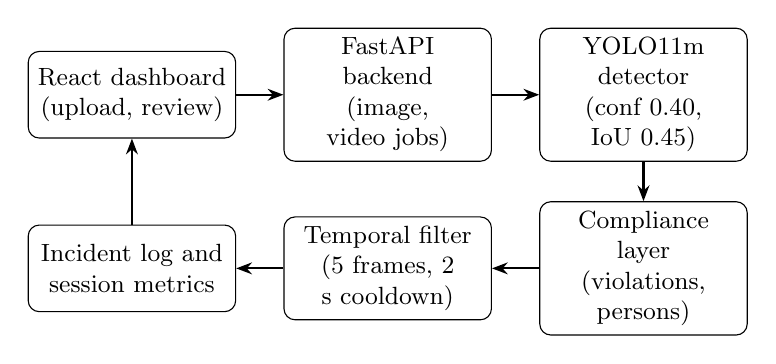
\begin{tikzpicture}[
  node distance=5mm and 6mm,
  box/.style={draw, rounded corners, align=center, font=\small, minimum height=11mm, text width=24mm},
  arr/.style={-{Stealth[length=2mm]}, thick}]
\node[box] (ui) {React dashboard\\(upload, review)};
\node[box, right=of ui] (api) {FastAPI backend\\(image, video jobs)};
\node[box, right=of api] (det) {YOLO11m detector\\(conf 0.40, IoU 0.45)};
\node[box, below=of det] (rule) {Compliance layer\\(violations, persons)};
\node[box, left=of rule] (temp) {Temporal filter\\(5 frames, 2 s cooldown)};
\node[box, left=of temp] (log) {Incident log and\\session metrics};
\draw[arr] (ui) -- (api);
\draw[arr] (api) -- (det);
\draw[arr] (det) -- (rule);
\draw[arr] (rule) -- (temp);
\draw[arr] (temp) -- (log);
\draw[arr] (log) -- (ui);
\end{tikzpicture}
\caption{Processing pipeline. Photos skip the temporal filter and raise an incident directly when a violation class is detected.}
\label{fig:architecture}
\end{figure}

\subsection{Detection classes}

The detector predicts the ten classes listed in \cref{tab:classes}. The dataset labels the absence of PPE as explicit classes (NO-Hardhat, NO-Safety Vest, NO-Mask), so violations can be detected directly instead of being inferred from a person box without a matching PPE box. In the deployed configuration, NO-Hardhat and NO-Safety Vest raise incidents, NO-Mask is reported as advisory only, and safety cones, machinery and vehicles provide site context.

\begin{table}[htbp]
\centering
\small
\caption{Detection classes and their role in the compliance layer.}
\label{tab:classes}
\begin{tabular}{@{}lll@{}}
\toprule
ID & Class & Role \\
\midrule
0 & Hardhat & Required PPE \\
1 & Mask & PPE, advisory \\
2 & NO-Hardhat & Violation, raises an incident \\
3 & NO-Mask & Advisory, reported only \\
4 & NO-Safety Vest & Violation, raises an incident \\
5 & Person & Counted for the compliance score \\
6 & Safety Cone & Site context \\
7 & Safety Vest & Required PPE \\
8 & machinery & Site context \\
9 & vehicle & Site context \\
\bottomrule
\end{tabular}
\end{table}

\subsection{Detector architecture}

The detector is YOLO11m from the Ultralytics library\footnote{\url{https://github.com/ultralytics/ultralytics}}, initialised from COCO-pretrained weights \cite{lin2014coco}. Its backbone stacks strided convolutions and C3k2 blocks, followed by a spatial pyramid pooling block (SPPF) in the spirit of \cite{he2015spp} and a C2PSA attention block. The neck fuses three scales in a top-down and bottom-up path, following feature pyramid and path aggregation designs \cite{lin2017fpn,liu2018panet}, and an anchor-free decoupled head predicts boxes and class scores at strides 8, 16 and 32. With the ten-class head the model has 231 layers, 20,060,718 parameters and 68.3 GFLOPs at 640 px; after layer fusion for inference it has 125 layers, 20,037,742 parameters and 67.8 GFLOPs. All 649 pretrained parameter tensors were transferred; the classification head was resized from 80 to ten classes, and its Person row was initialised from the matching COCO class. Training minimises the weighted sum of a box regression loss, a classification loss and a distribution focal loss,
\begin{equation}
\mathcal{L} = \lambda_{\text{box}} \mathcal{L}_{\text{box}} + \lambda_{\text{cls}} \mathcal{L}_{\text{cls}} + \lambda_{\text{dfl}} \mathcal{L}_{\text{dfl}},
\label{eq:loss}
\end{equation}
with $\lambda_{\text{box}} = 7.5$, $\lambda_{\text{cls}} = 0.5$ and $\lambda_{\text{dfl}} = 1.5$.

\subsection{Compliance rule and temporal confirmation}

For a frame $t$ with detected class set $D_t$, the set of violations is $V_t = D_t \cap \{\text{NO-Hardhat}, \text{NO-Safety Vest}\}$. The frame counts $p_t$ persons and is marked compliant when at least one person is present and both required items are detected,
\begin{equation}
c_t = \begin{cases} 1 & \text{if } p_t > 0 \text{ and } \{\text{Hardhat}, \text{Safety Vest}\} \subseteq D_t, \\ 0 & \text{otherwise.} \end{cases}
\label{eq:compliance}
\end{equation}
The session compliance score is $S = 100 \sum_t c_t / \sum_t p_t$. Because $c_t$ is at most one per frame, $S$ is a frame-level approximation that understates compliance in frames with several compliant workers; per-person association is left to future work (\cref{sec:conclusion}).

In video, a violation class $v$ is confirmed at frame $t$ only if it was detected in each of the last $W$ frames,
\begin{equation}
v \in C_t \iff v \in V_{t-k} \quad \text{for all } k = 0, \ldots, W-1,
\label{eq:temporal}
\end{equation}
with $W = 5$. A confirmed violation creates an incident with an annotated snapshot, and a 2 s cooldown prevents repeated incidents for the same event. Single photos have no temporal context, so any detected violation raises an incident directly. The confidence and non-maximum suppression thresholds default to 0.40 and 0.45 and can be changed from the dashboard within the range 0.10 to 0.95.

\section{Experimental setup}
\label{sec:setup}

\subsection{Dataset and split}

The experiments use the Construction Site Safety Image Dataset distributed through Roboflow and Kaggle\footnote{\url{https://www.kaggle.com/datasets/snehilsanyal/construction-site-safety-image-dataset-roboflow}}, which provides YOLO-format labels for the ten classes in \cref{tab:classes}. The original train, validation and test folders were pooled and re-split 80/10/10 with scikit-learn, stratified by each image's dominant class with a fixed seed of 42. Dominant-class groups with fewer than five images were merged into a background group so that every group could be split. \Cref{tab:split} gives the resulting image and box counts.

\begin{table}[htbp]
\centering
\small
\caption{Images and annotated boxes per split after the stratified 80/10/10 re-split.}
\label{tab:split}
\begin{tabular}{@{}lrrr@{}}
\toprule
Split & Images & Share & Boxes \\
\midrule
Train & 2,240 & 80.0\% & 30,684 \\
Validation & 280 & 10.0\% & 3,554 \\
Test & 281 & 10.0\% & 4,114 \\
\midrule
Total & 2,801 & 100\% & 38,352 \\
\bottomrule
\end{tabular}
\end{table}

\Cref{fig:classdist} shows the number of boxes per class in each split. Every class keeps a similar share across the three splits, which confirms that the stratification worked. The dataset is imbalanced: Person has 9,872 boxes in total, about six times as many as vehicle (1,628) or Mask (1,700).

\begin{figure}[htbp]
\centering
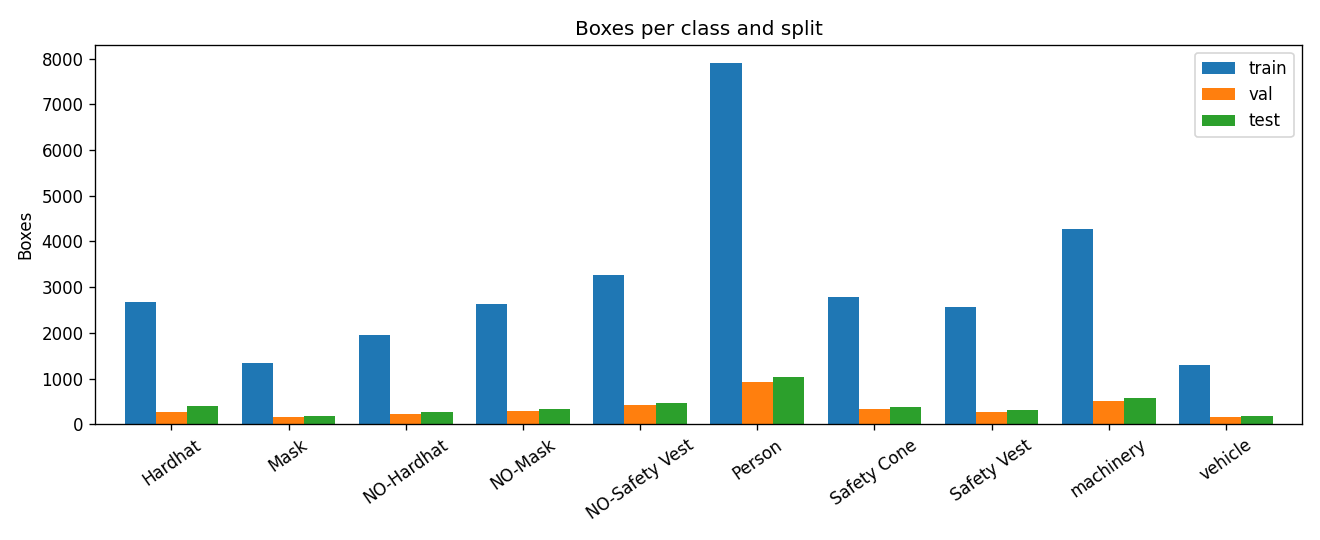
\includegraphics[width=\linewidth,height=0.4\textheight,keepaspectratio]{class_distribution.png}
\caption{Annotated boxes per class in the train, validation and test splits.}
\label{fig:classdist}
\end{figure}

\subsection{Training configuration}

Training ran on Kaggle with two NVIDIA Tesla T4 GPUs (15 GB each), 4 CPU cores and 33.7 GB of RAM, using Ultralytics 8.4.171, PyTorch 2.10.0 and CUDA 12.8. Both GPUs were used through PyTorch distributed data-parallel training \cite{li2020ddp} with automatic mixed precision. The run was given a wall-clock budget of 0.70 h rather than a fixed epoch count; the library fitted the epoch count and the cosine learning-rate schedule to that budget, with 200 epochs as an upper bound. \Cref{tab:hyper} lists the main hyperparameters.

\begin{table}[htbp]
\centering
\small
\caption{Training hyperparameters, as recorded in the training log (LR: learning rate).}
\label{tab:hyper}
\begin{tabular*}{\linewidth}{@{\extracolsep{\fill}}llll@{}}
\toprule
Parameter & Value & Parameter & Value \\
\midrule
Input size & 640 px & Optimiser & SGD \\
Batch size & 32 (16 per GPU) & Momentum & 0.937 \\
Time budget & 0.70 h & Initial LR & 0.01 \\
Epoch limit & 200 (upper bound) & Final LR factor & 0.01 \\
Warm-up & 3 epochs & LR schedule & Cosine \\
Mosaic & 1.0 & Weight decay & 0.0005 \\
Mosaic off & Last 10 epochs & Patience & 100 epochs \\
Mixup / copy-paste & 0.1 / 0.1 & Translation / scale & 0.1 / 0.5 \\
Rotation / shear & 5.0 / 2.0 degrees & HSV (h, s, v) & 0.015, 0.7, 0.4 \\
Horizontal flip & 0.5 & Image cache & RAM \\
Mixed precision & Yes (AMP) & Seed & 42 \\
\bottomrule
\end{tabular*}
\end{table}

\Cref{fig:gpu} shows the utilisation and memory of both GPUs, sampled every 30 s during training. Utilisation of both GPUs stayed mostly between 85\% and 100\%, with a few short dips, and memory use held at about 8.3 GB per GPU apart from brief periodic drops, with peaks of 8,677 MB and 8,543 MB out of 15,360 MB.

\begin{figure}[htbp]
\centering
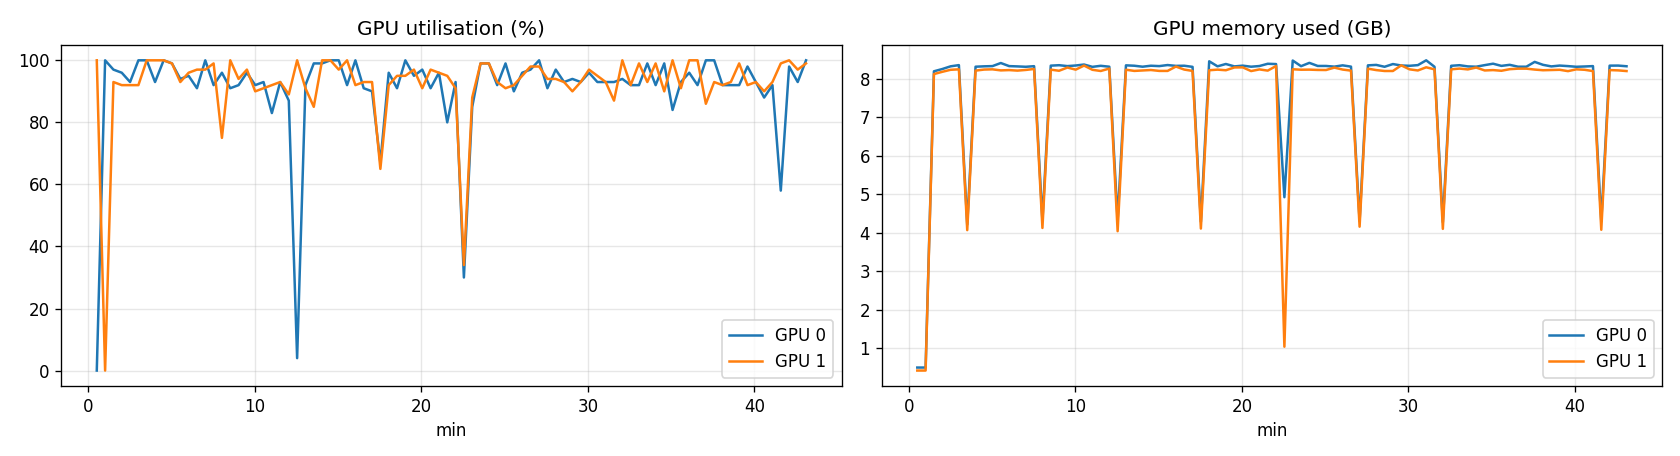
\includegraphics[width=\linewidth,height=0.4\textheight,keepaspectratio]{gpu_usage.png}
\caption{Utilisation and memory use of the two T4 GPUs during training.}
\label{fig:gpu}
\end{figure}

\subsection{Evaluation protocol}

The checkpoint with the best validation fitness (\texttt{best.pt}) was evaluated on the validation and test splits at 640 px with half precision and a batch size of 16, and the test split was evaluated again with flip and scale TTA. For each class, average precision (AP) is the area under the precision-recall curve, where a prediction is a true positive when its intersection over union (IoU) with a ground-truth box of the same class reaches the threshold \cite{everingham2010voc}. mAP@0.5 averages AP over classes at an IoU of 0.5, and mAP@0.5:0.95 also averages over IoU thresholds from 0.5 to 0.95 in steps of 0.05, following COCO \cite{lin2014coco}. Precision $P$ and recall $R$ are reported at the confidence that maximises the mean F1 score, and the summary F1 is
\begin{equation}
F_1 = \frac{2PR}{P + R}.
\label{eq:f1}
\end{equation}
Latency is the model inference time per image reported by the evaluator on one T4.

\section{Results and discussion}
\label{sec:results}

\subsection{Training behaviour}

The run completed 75 epochs in 0.701 h. \Cref{fig:training} plots the losses, precision, recall, mAP and learning rate per epoch. Training losses fall steadily, with a visible step down at epoch 66 when mosaic augmentation is switched off. Validation losses rise briefly in epochs 3 to 6 just after warm-up, then fall and level off after about epoch 60. The best epoch was 72, with a validation mAP@0.5 of 0.8692 and mAP@0.5:0.95 of 0.6375, and from epoch 68 onward validation mAP@0.5:0.95 stayed between 0.632 and 0.638, so training ended on a plateau rather than being cut off while still improving. The learning rate decays from its warm-up peak to $1.04 \times 10^{-4}$ at epoch 75.

\begin{figure}[htbp]
\centering
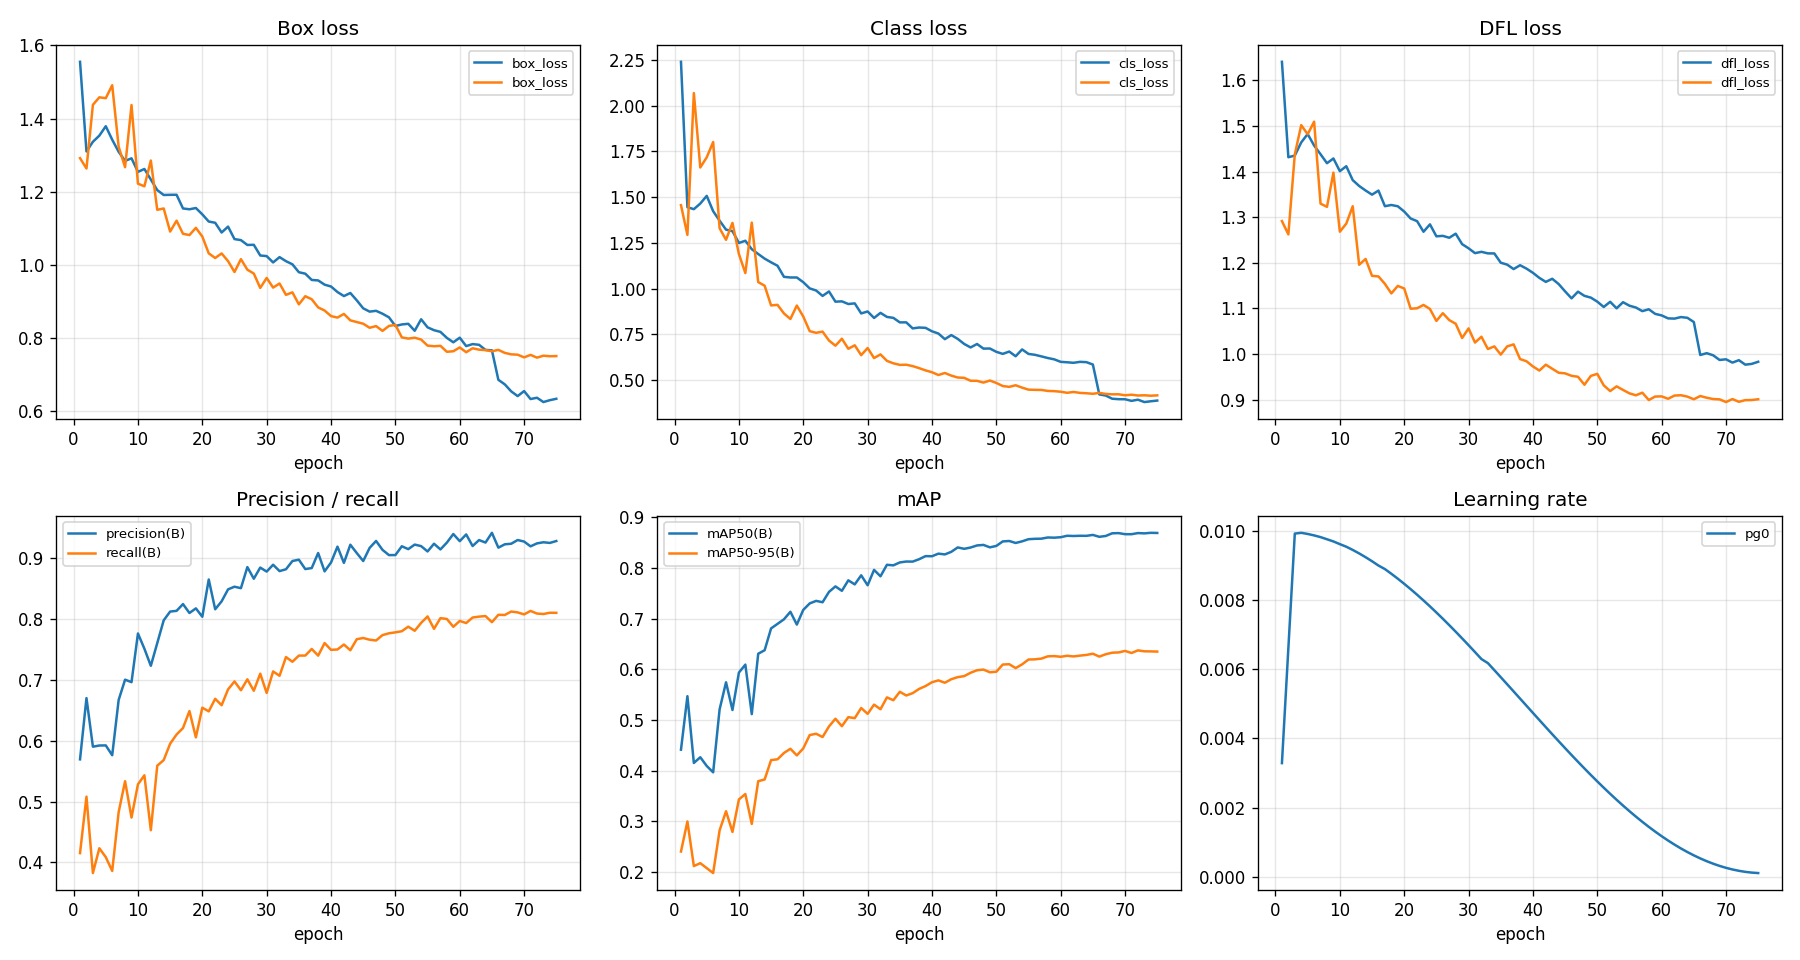
\includegraphics[width=\linewidth,height=0.4\textheight,keepaspectratio]{training_curves.png}
\caption{Per-epoch box, classification and distribution focal losses (training in blue, validation in orange), validation precision and recall, validation mAP, and learning rate.}
\label{fig:training}
\end{figure}

\subsection{Overall detection accuracy}

\Cref{tab:overall} summarises accuracy and latency. On the held-out test split, the model reaches an mAP@0.5 of 0.8659 and an mAP@0.5:0.95 of 0.6158, close to the validation values of 0.8679 and 0.6368. The small gap between validation and test suggests that the checkpoint selection did not overfit the validation split. Precision (0.9135) is clearly higher than recall (0.8053) on the test split, so the model's errors are mostly missed objects rather than false alarms at the operating point used for these figures.

\begin{table}[htbp]
\centering
\small
\caption{Overall accuracy and inference latency of \texttt{best.pt} (640 px, fp16, batch 16, one T4).}
\label{tab:overall}
\setlength{\tabcolsep}{4pt}
\begin{tabular}{@{}lcccccc@{}}
\toprule
Split & mAP@0.5 & mAP@0.5:0.95 & Precision & Recall & F1 & ms/img \\
\midrule
Validation & 0.8679 & 0.6368 & 0.9236 & 0.8084 & 0.8621 & 32.79 \\
Test & 0.8659 & 0.6158 & 0.9135 & 0.8053 & 0.8560 & 31.32 \\
Test with TTA & 0.8603 & 0.6206 & 0.9027 & 0.7853 & 0.8399 & 85.98 \\
\bottomrule
\end{tabular}
\end{table}

TTA lowered mAP@0.5 from 0.8659 to 0.8603, precision from 0.9135 to 0.9027 and recall from 0.8053 to 0.7853, and raised only mAP@0.5:0.95, from 0.6158 to 0.6206. It took 85.98 ms per image, 2.7 times the 31.32 ms of plain inference. For a monitoring system that must keep up with video, TTA is therefore not worthwhile, and the deployed backend does not use it. In the final validation inside the training run, preprocessing, inference and postprocessing took 1.3 ms, 15.0 ms and 6.2 ms per image. Predicting all 281 test images, with 4,002 boxes drawn, ran at 35.9 images per second end to end.

\Cref{fig:testcurves} shows the precision, recall, F1 and precision-recall curves for the test split; the validation-split curves are in \cref{fig:valcurves} in the appendix. On the test split, the all-class F1 curve peaks at 0.85 at a confidence of 0.362 and stays close to that value over a broad plateau, so the deployed default of 0.40 lies in a stable region rather than on a sharp optimum.

\begin{figure}[htbp]
\centering
\begin{subfigure}{0.42\linewidth}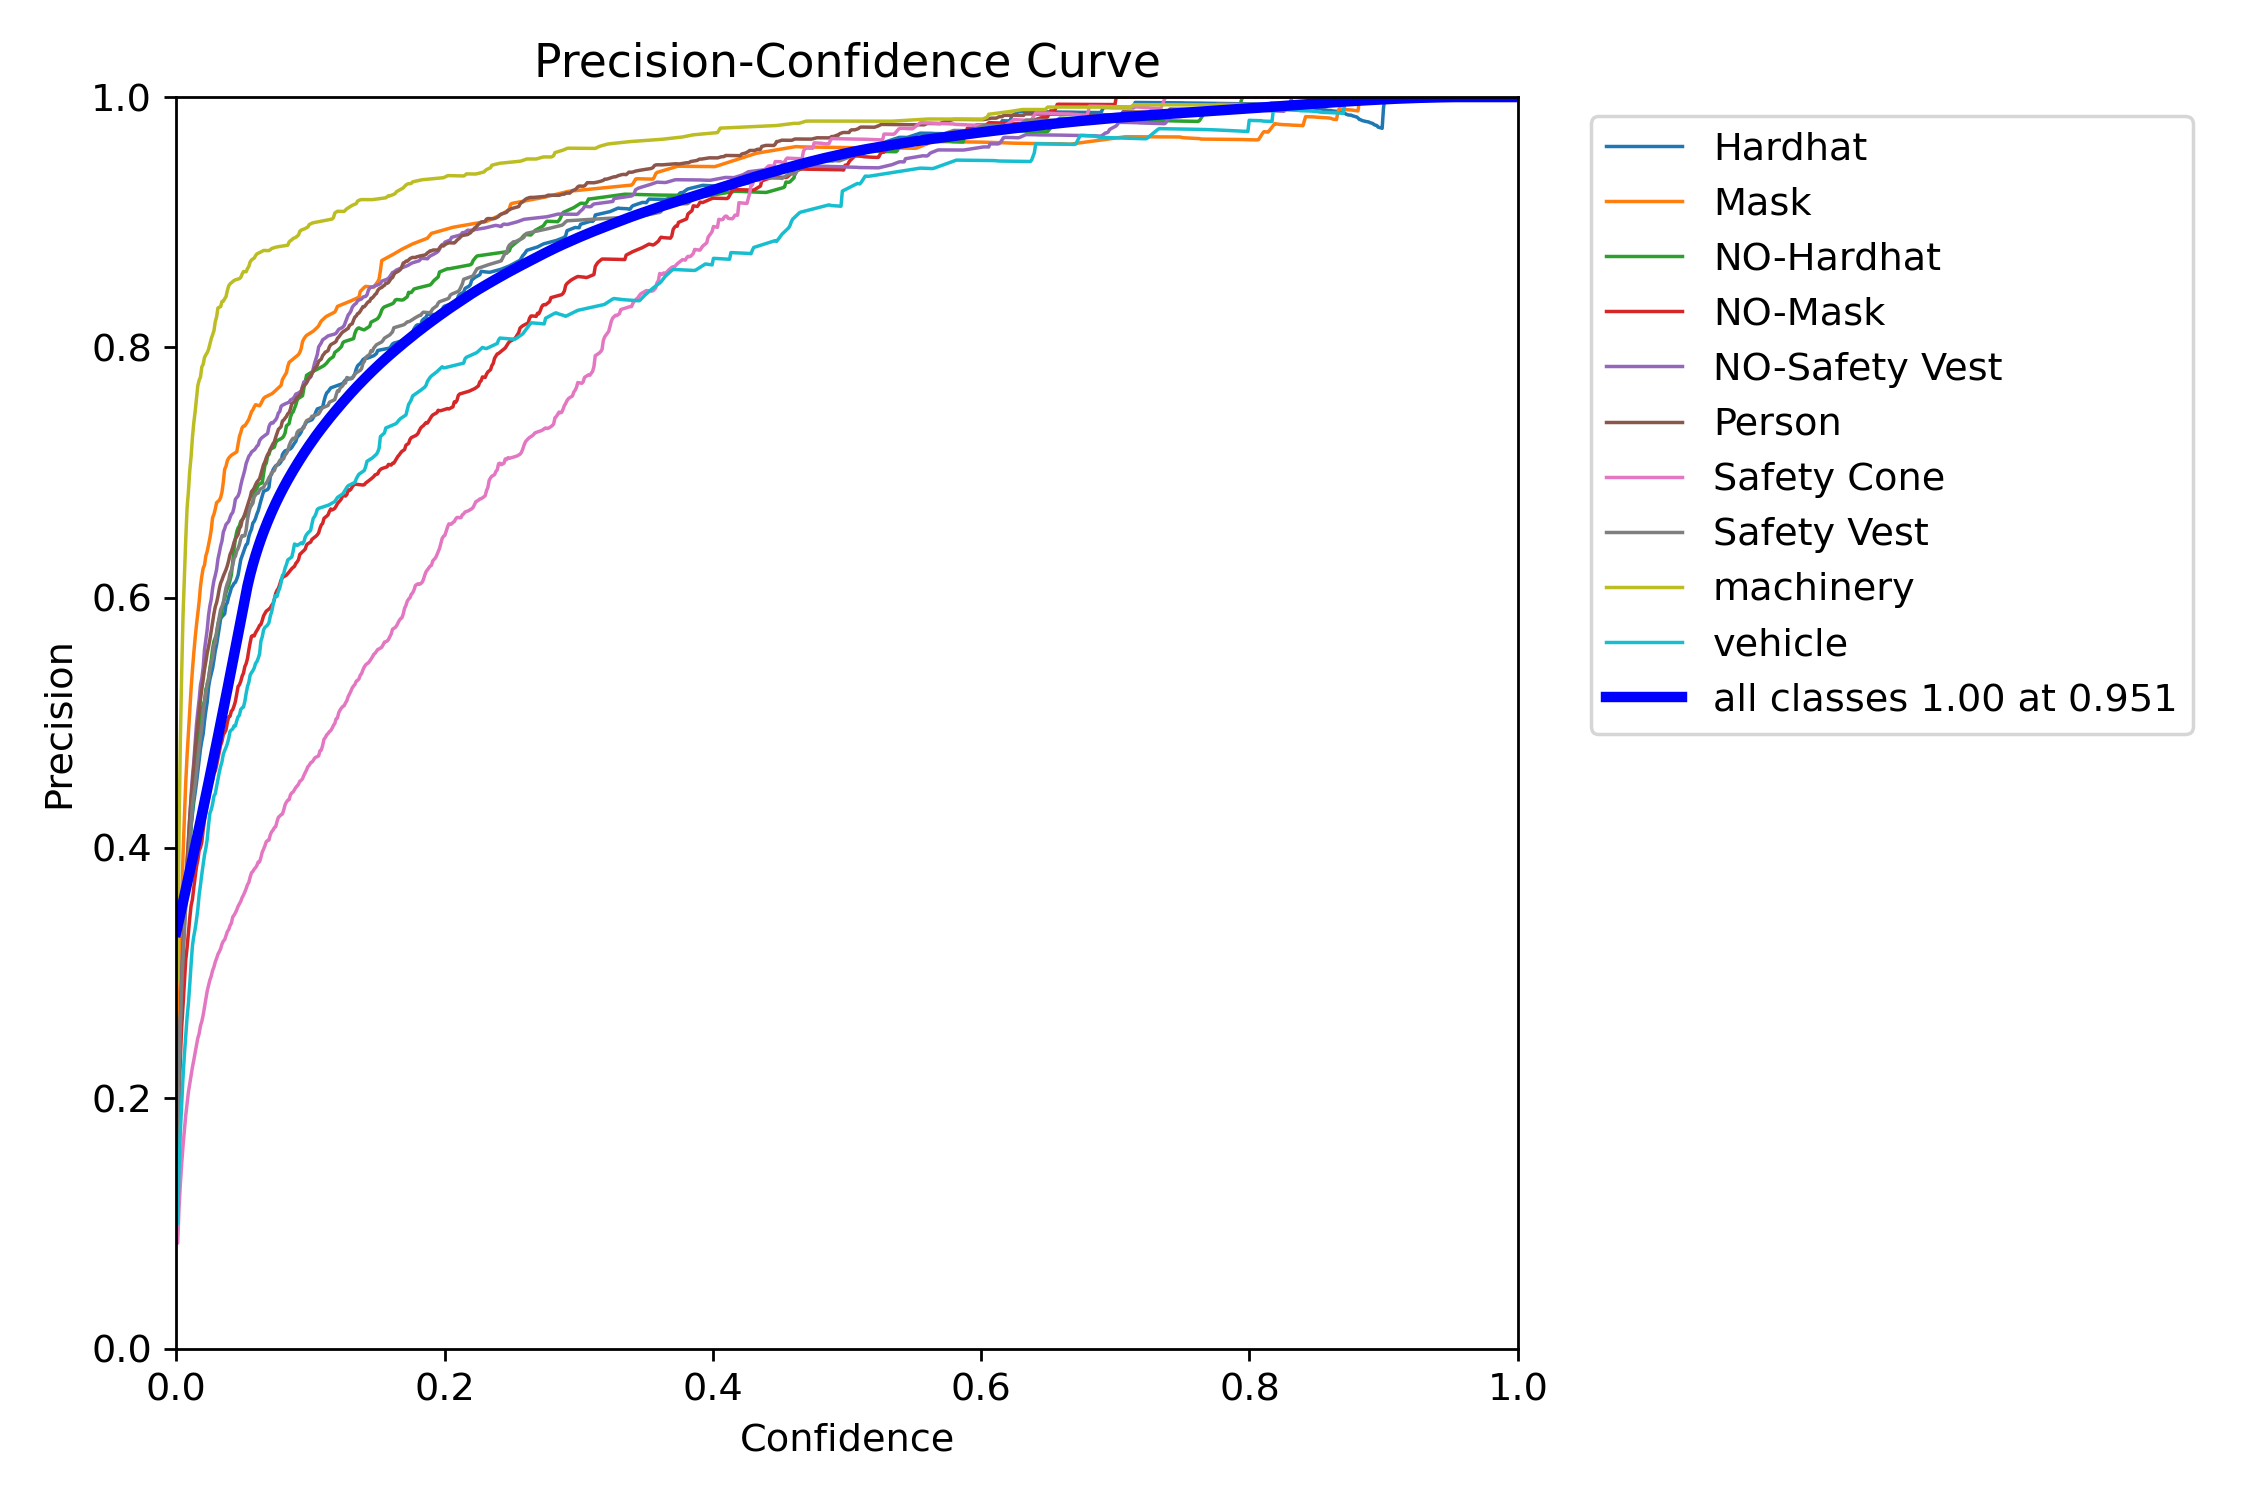
\includegraphics[width=\linewidth]{eval_test_BoxP_curve.png}\caption{Precision}\end{subfigure}\hspace{4mm}
\begin{subfigure}{0.42\linewidth}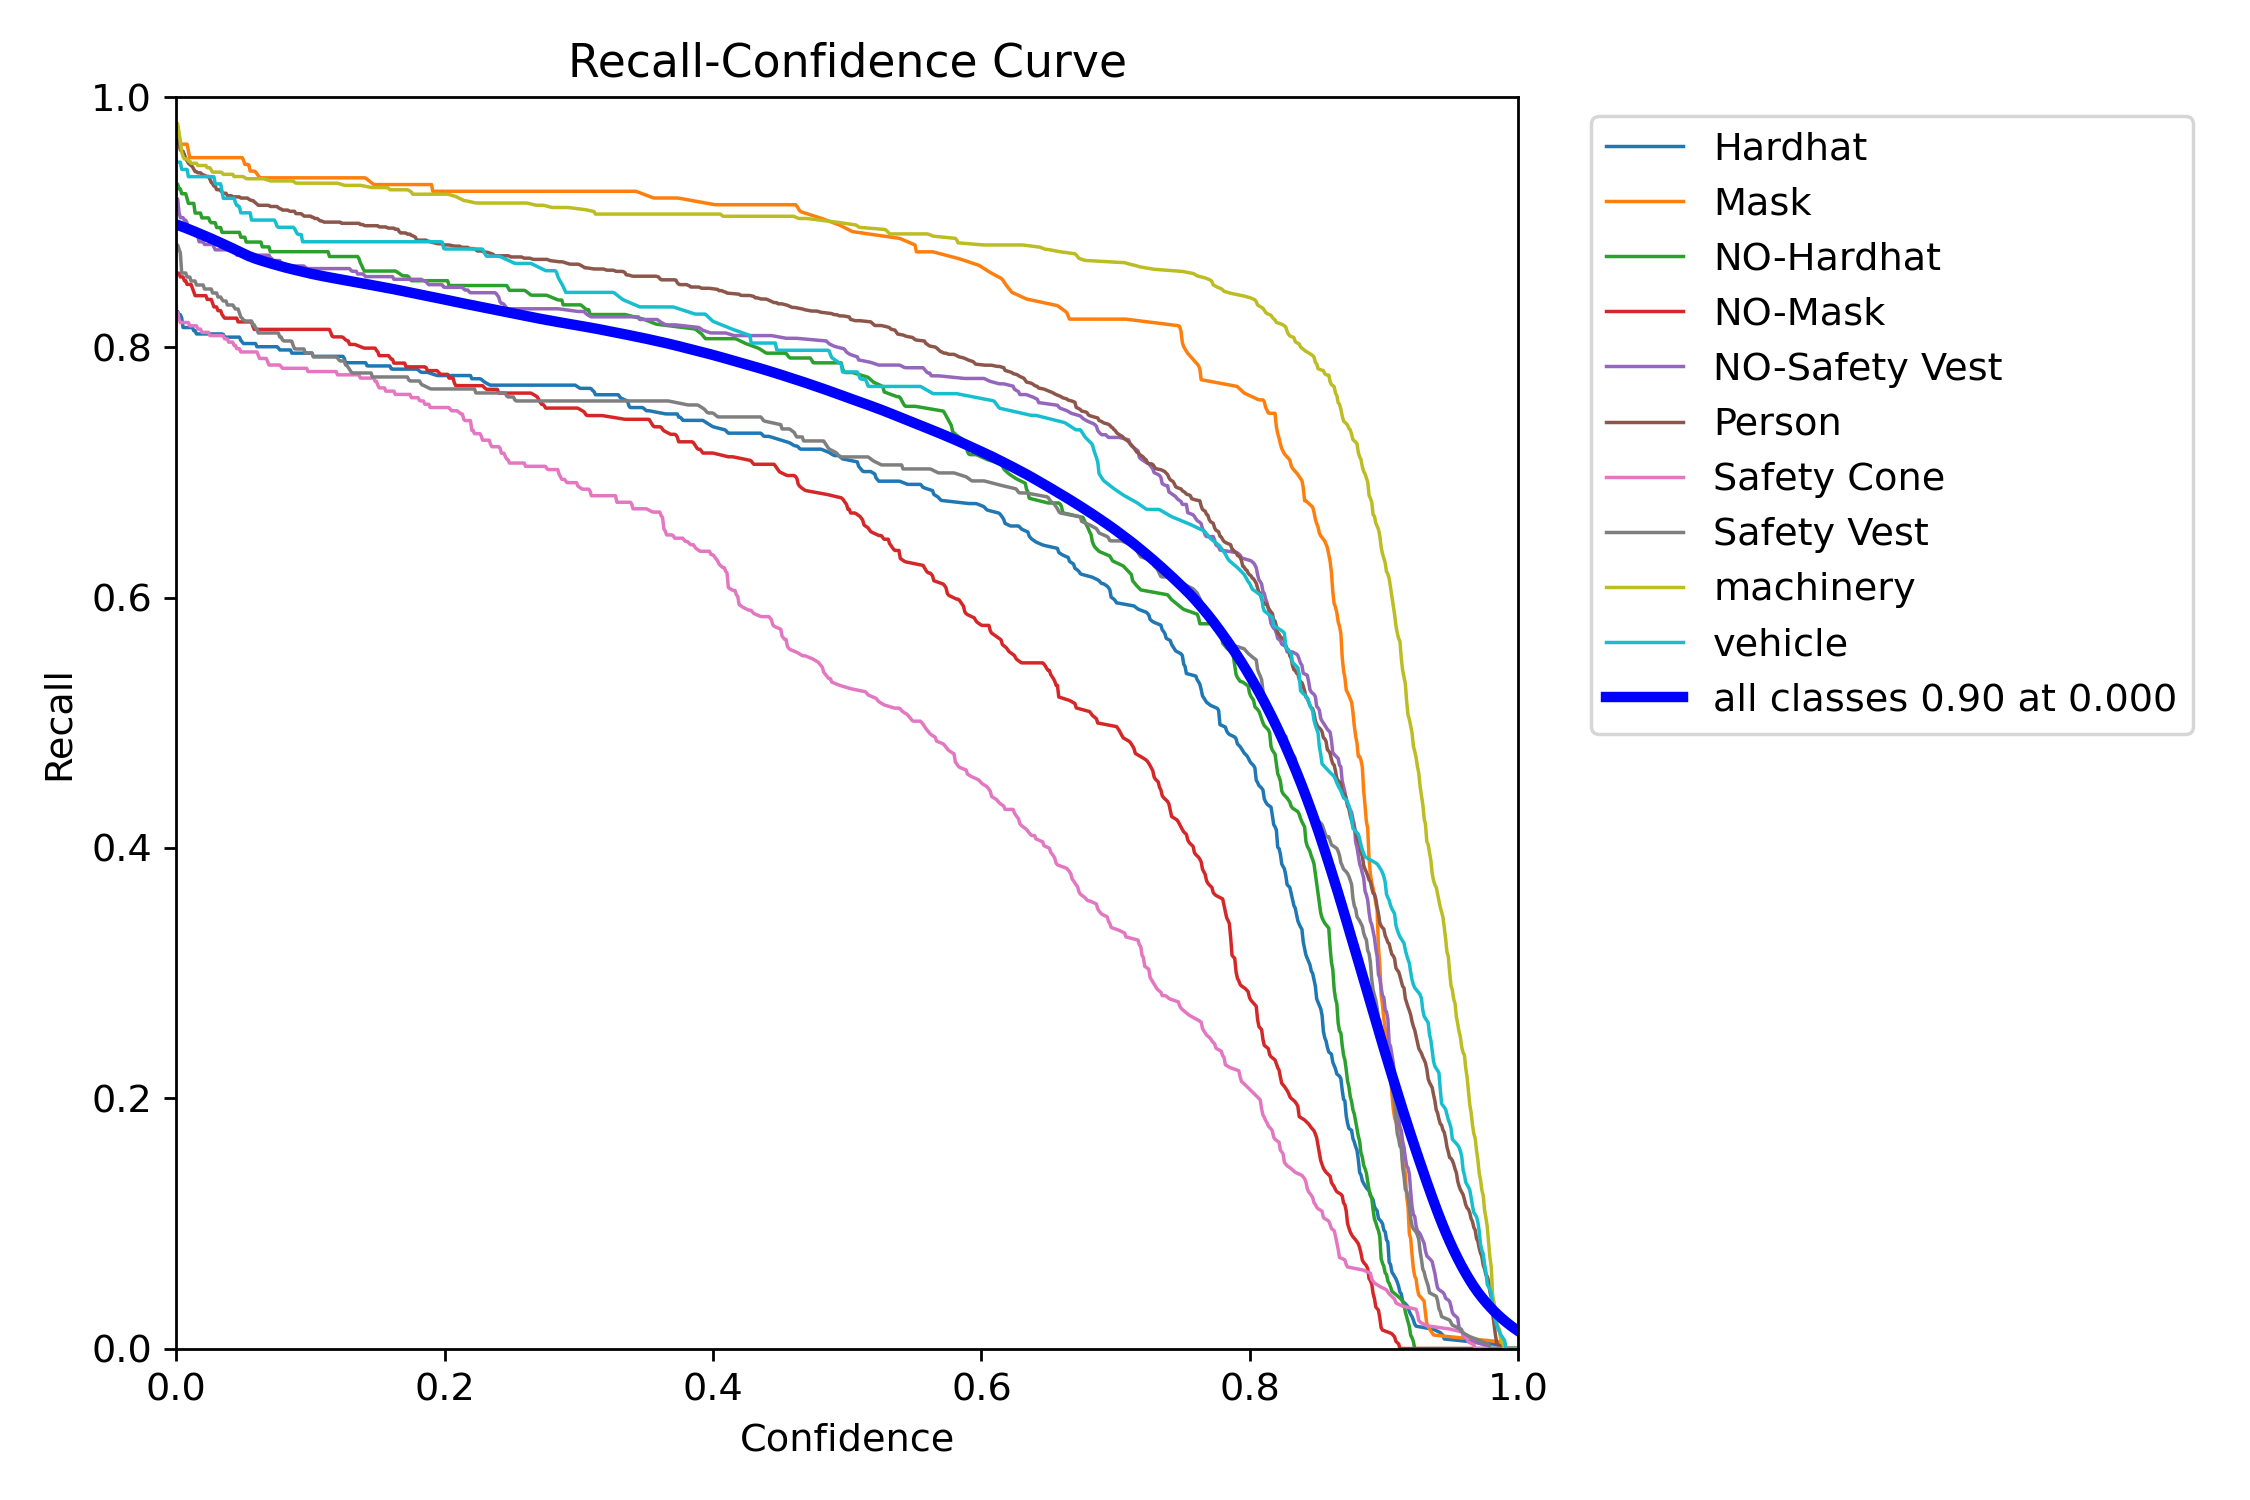
\includegraphics[width=\linewidth]{eval_test_BoxR_curve.png}\caption{Recall}\end{subfigure}\\[2mm]
\begin{subfigure}{0.42\linewidth}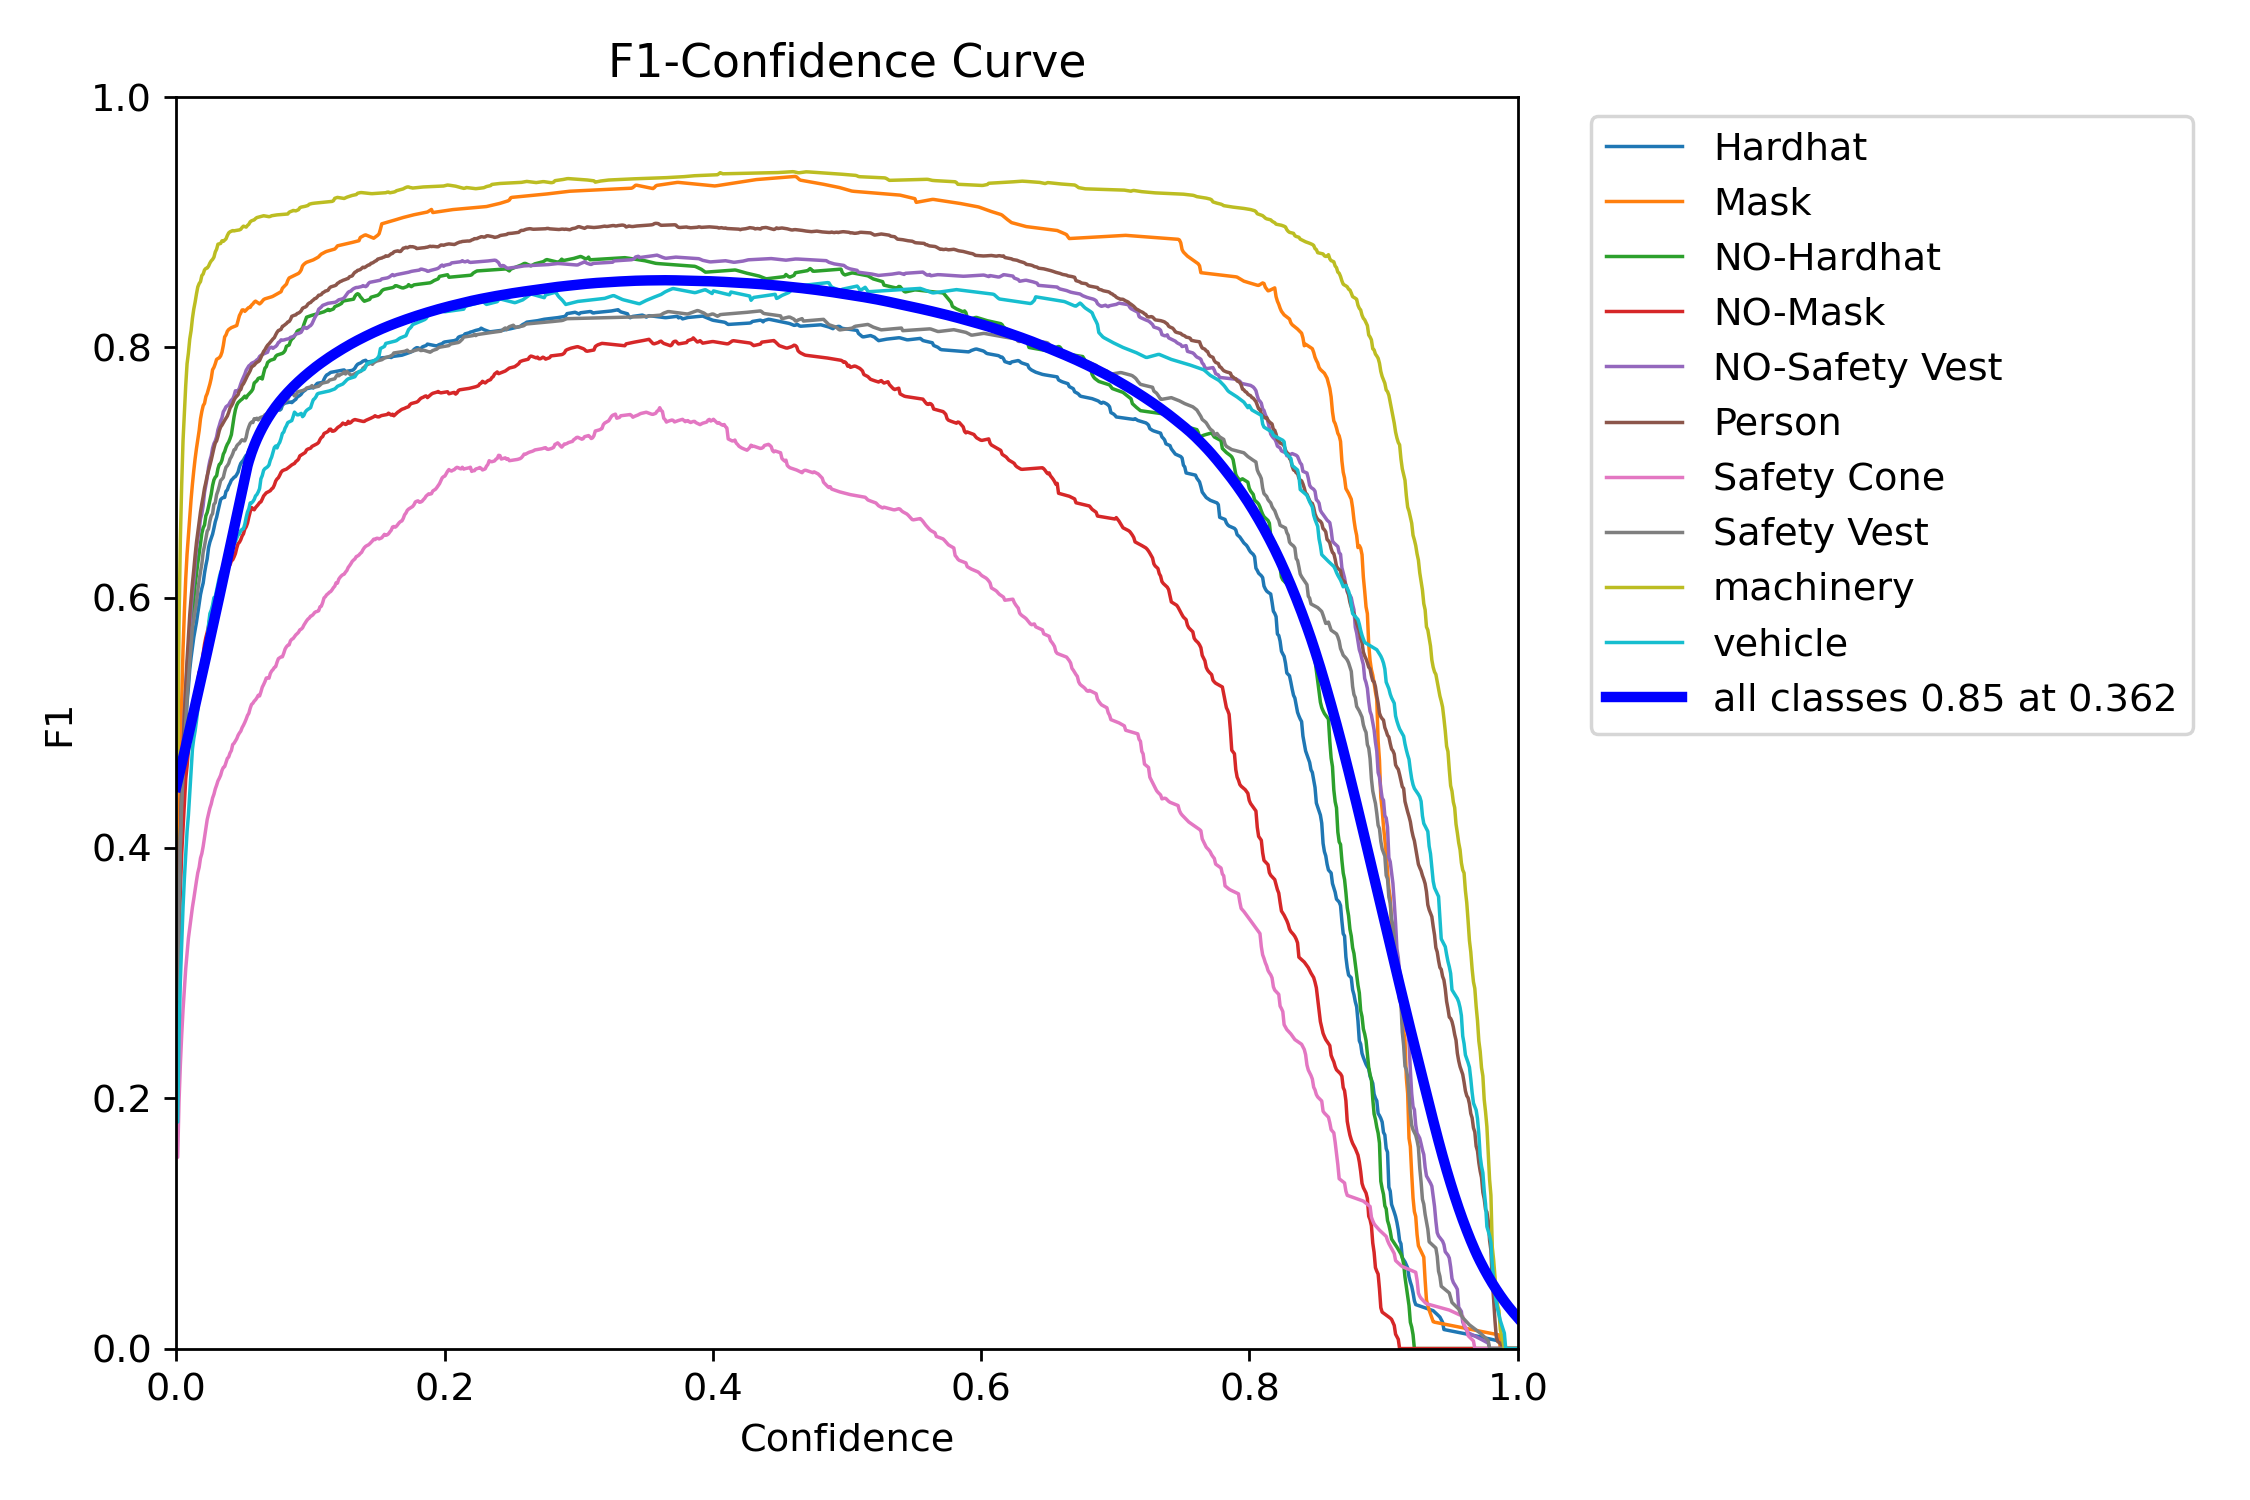
\includegraphics[width=\linewidth]{eval_test_BoxF1_curve.png}\caption{F1}\end{subfigure}\hspace{4mm}
\begin{subfigure}{0.42\linewidth}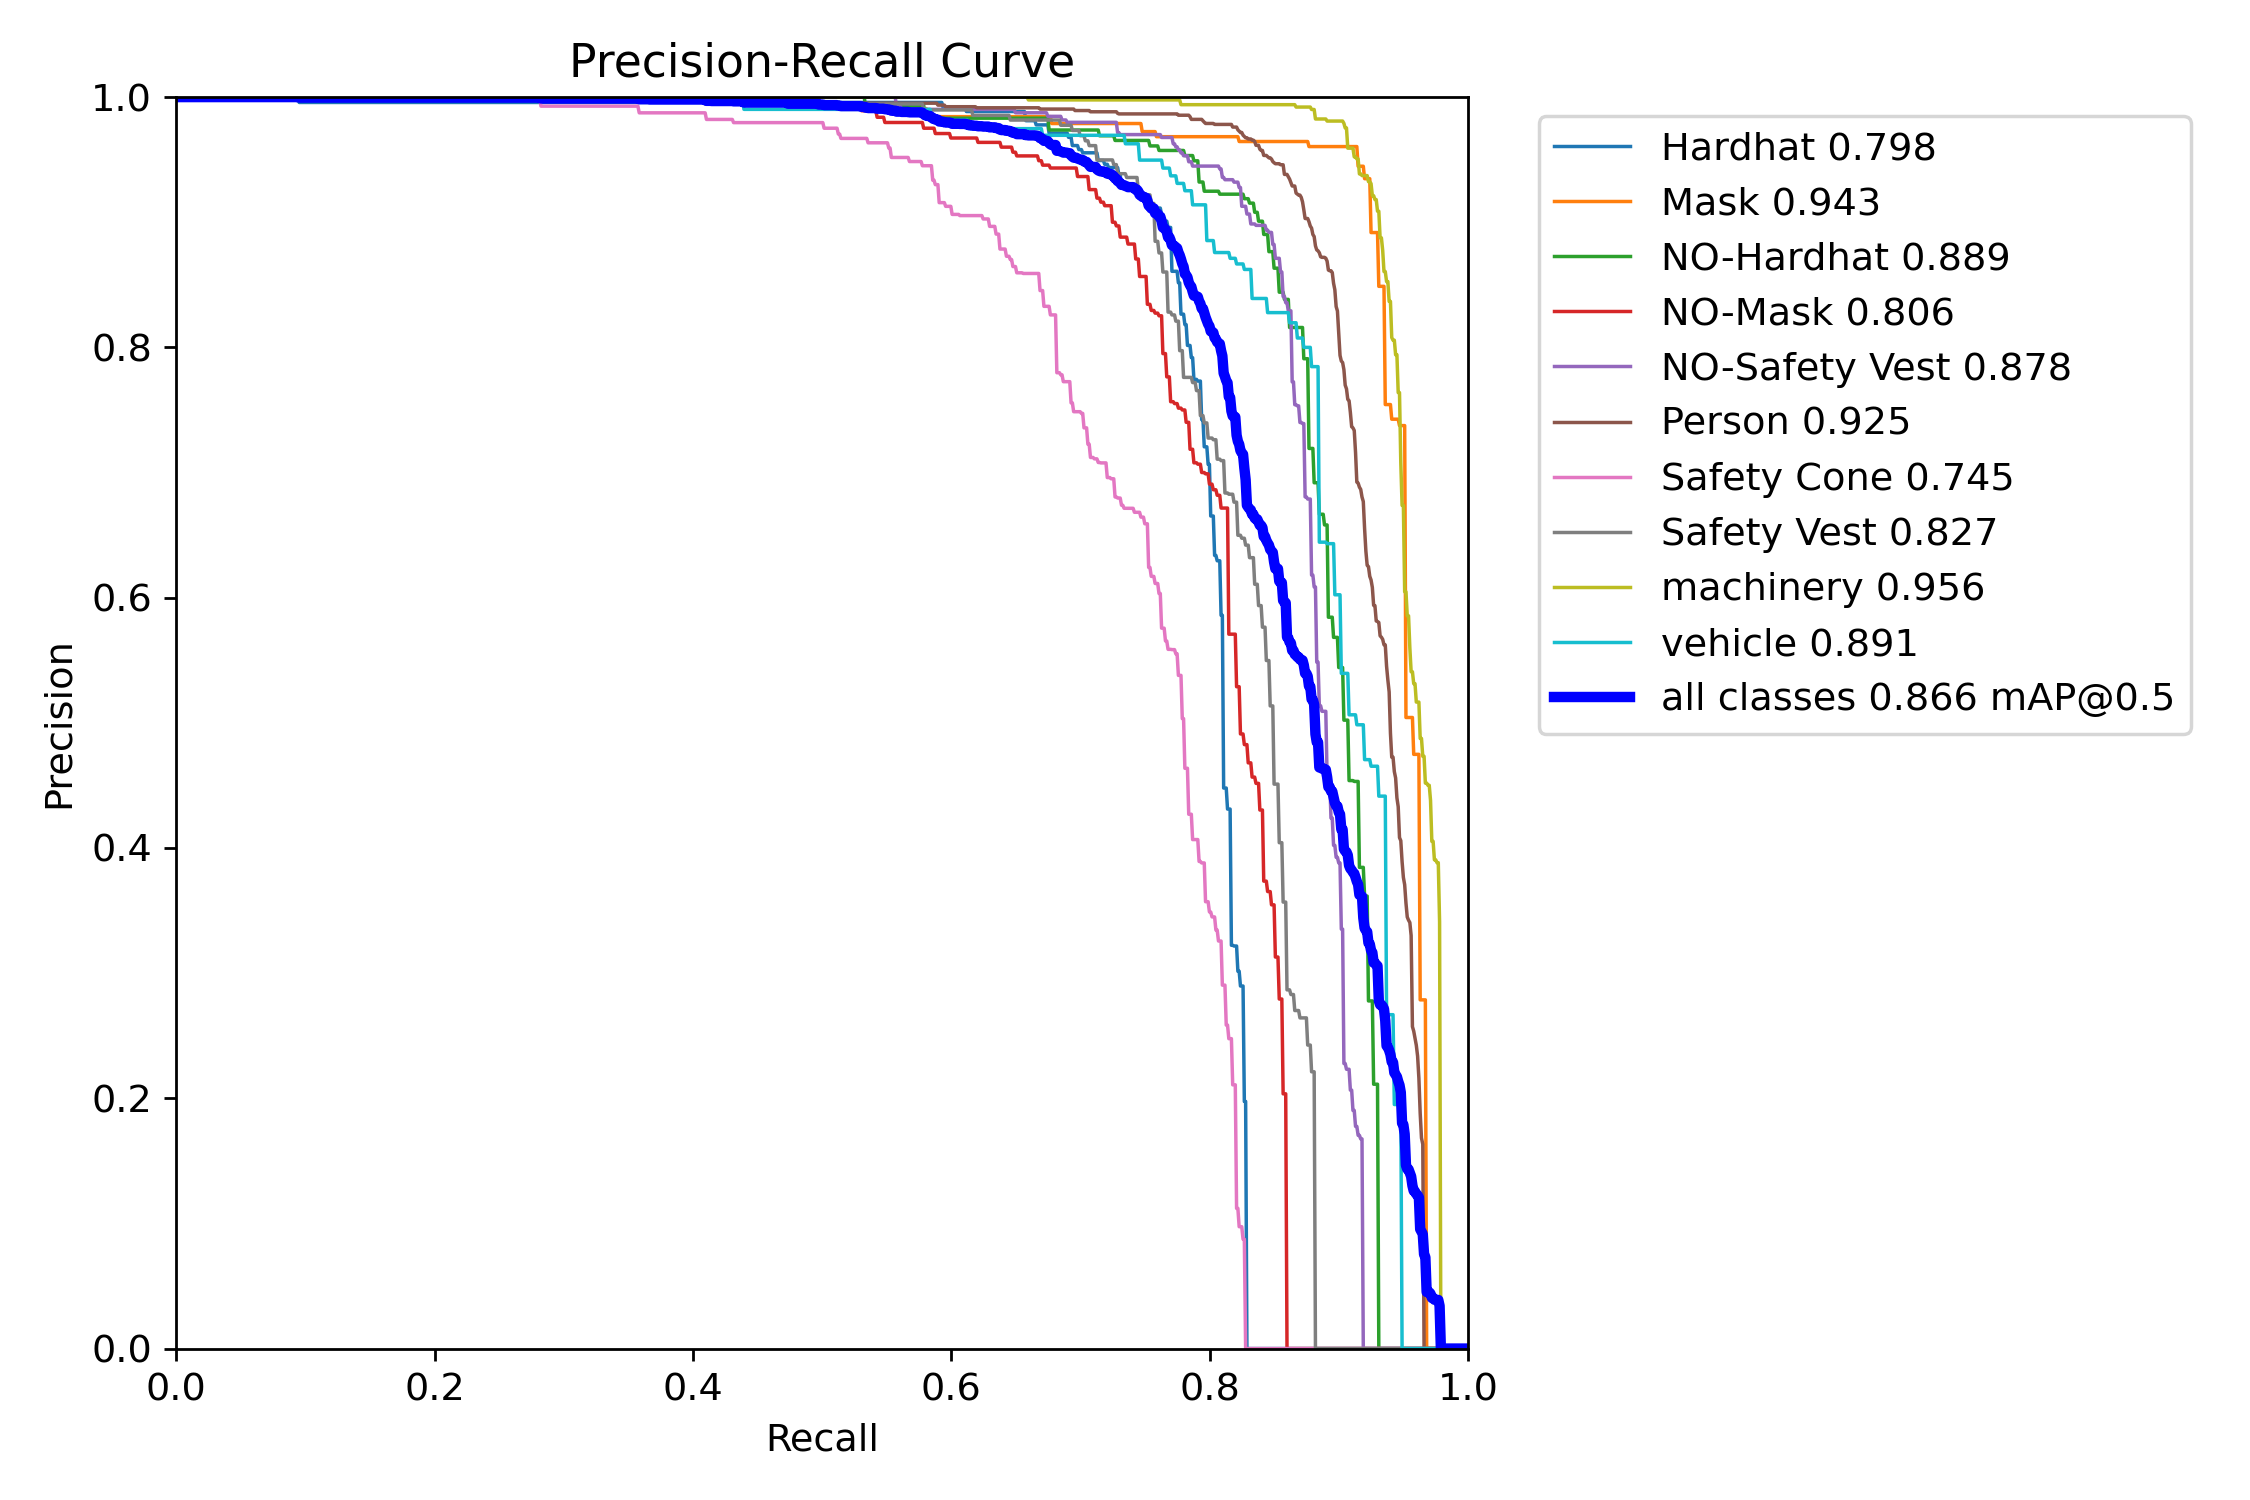
\includegraphics[width=\linewidth]{eval_test_BoxPR_curve.png}\caption{Precision-recall}\end{subfigure}
\caption{Held-out test split (281 images): precision, recall and F1 against confidence, and the precision-recall curve per class.}
\label{fig:testcurves}
\end{figure}

\subsection{Per-class accuracy}

\Cref{tab:perclass} breaks accuracy down by class for the validation and test splits.

\begin{center}
\begin{minipage}{\linewidth}
\centering
\small
\captionsetup{hypcap=false}
\captionof{table}{Per-class AP@0.5 (AP50), AP@0.5:0.95 (AP), precision (P) and recall (R) on the validation and test splits.}
\label{tab:perclass}
\setlength{\tabcolsep}{4pt}
\begin{tabular}{@{}lcccccccc@{}}
\toprule
& \multicolumn{4}{c}{Validation} & \multicolumn{4}{c}{Test} \\
\cmidrule(lr){2-5}\cmidrule(l){6-9}
Class & AP50 & AP & P & R & AP50 & AP & P & R \\
\midrule
Hardhat & 0.8592 & 0.6170 & 0.9339 & 0.8188 & 0.7975 & 0.5420 & 0.9183 & 0.7473 \\
Mask & 0.9763 & 0.7667 & 0.9609 & 0.9345 & 0.9432 & 0.7137 & 0.9411 & 0.9194 \\
NO-Hardhat & 0.8676 & 0.5992 & 0.9188 & 0.8043 & 0.8894 & 0.5813 & 0.9217 & 0.8179 \\
NO-Mask & 0.8249 & 0.5129 & 0.9209 & 0.7433 & 0.8055 & 0.4587 & 0.8878 & 0.7346 \\
NO-Safety Vest & 0.9034 & 0.6753 & 0.9161 & 0.8535 & 0.8782 & 0.6445 & 0.9318 & 0.8194 \\
Person & 0.9290 & 0.7275 & 0.9638 & 0.8581 & 0.9250 & 0.7124 & 0.9459 & 0.8540 \\
Safety Cone & 0.7027 & 0.3969 & 0.8468 & 0.6172 & 0.7447 & 0.3963 & 0.8583 & 0.6641 \\
Safety Vest & 0.8317 & 0.6284 & 0.9388 & 0.7820 & 0.8273 & 0.5983 & 0.9103 & 0.7572 \\
machinery & 0.9555 & 0.8290 & 0.9520 & 0.9109 & 0.9565 & 0.8325 & 0.9663 & 0.9065 \\
vehicle & 0.8288 & 0.6155 & 0.8839 & 0.7612 & 0.8914 & 0.6781 & 0.8538 & 0.8324 \\
\bottomrule
\end{tabular}
\end{minipage}
\end{center}

Machinery (test AP@0.5 0.9565), Mask (0.9432) and Person (0.9250) are detected best. Safety Cone is the weakest class on every split, with a test AP@0.5 of 0.7447 and an AP@0.5:0.95 of only 0.3963, which reflects how small and thin cones usually are in site images. Hardhat drops from 0.8592 on validation to 0.7975 on test, the largest validation-to-test drop of any class, and NO-Mask (0.8055) and Safety Vest (0.8273) are also below the mean. For compliance monitoring the two incident classes matter most: NO-Hardhat reaches a test AP@0.5 of 0.8894 and NO-Safety Vest 0.8782, both above the overall mean.

\Cref{fig:perclassap} compares per-class AP@0.5 across the validation split, the test split and the test split with TTA. TTA changes most classes by less than 0.01; the largest change is a drop for Safety Cone, from 0.7447 to 0.7146, so augmentation at inference does not help the weakest class either.

\begin{figure}[htbp]
\centering
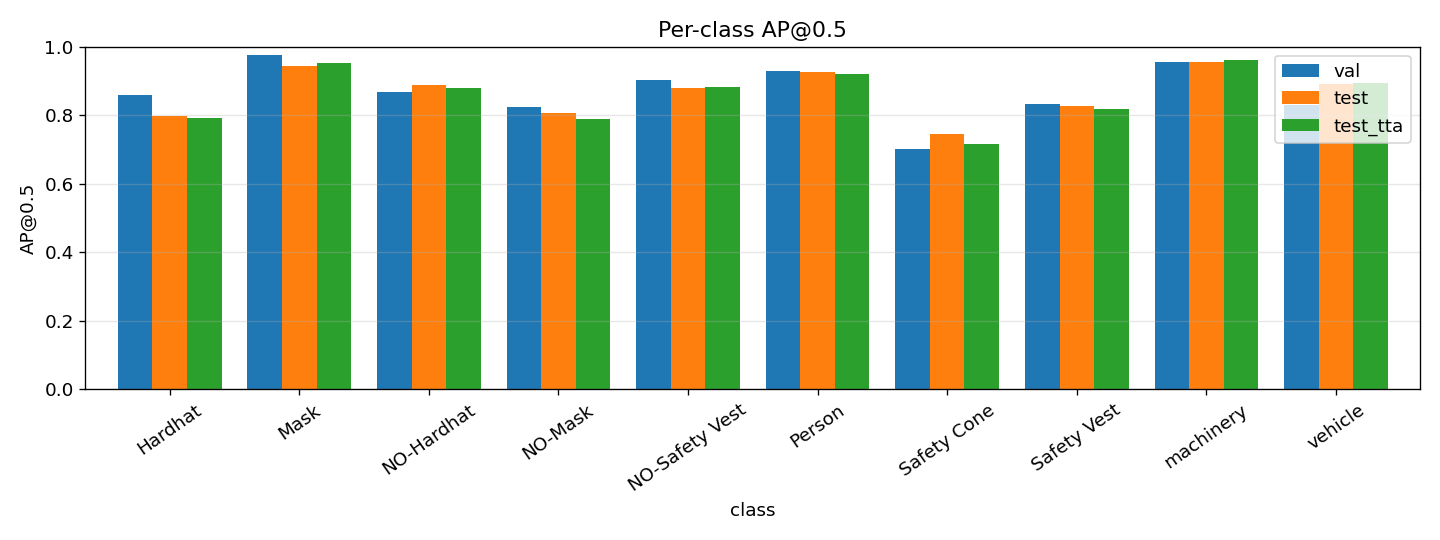
\includegraphics[width=\linewidth,height=0.4\textheight,keepaspectratio]{per_class_ap.png}
\caption{Per-class AP@0.5 on the validation split, the test split and the test split with TTA (\texttt{test\_tta}).}
\label{fig:perclassap}
\end{figure}

\subsection{Error analysis}

The confusion matrices in \cref{fig:testcm} show where errors come from on the test split; the validation matrices are in \cref{fig:valcm}. In the normalised test matrix, the diagonal ranges from 0.63 for Safety Vest to 0.96 for machinery. The largest single error is missed detection: 16\% of true Hardhat boxes and 14\% each of true Safety Cone and Safety Vest boxes are not detected at all (predicted as background), and 12\% of NO-Mask and 9\% of NO-Safety Vest boxes are missed. Among class swaps, 10\% of true Safety Vest boxes are predicted as Person, which is consistent with a vest being a region inside a person box.

\begin{figure}[htbp]
\centering
\begin{subfigure}{0.49\linewidth}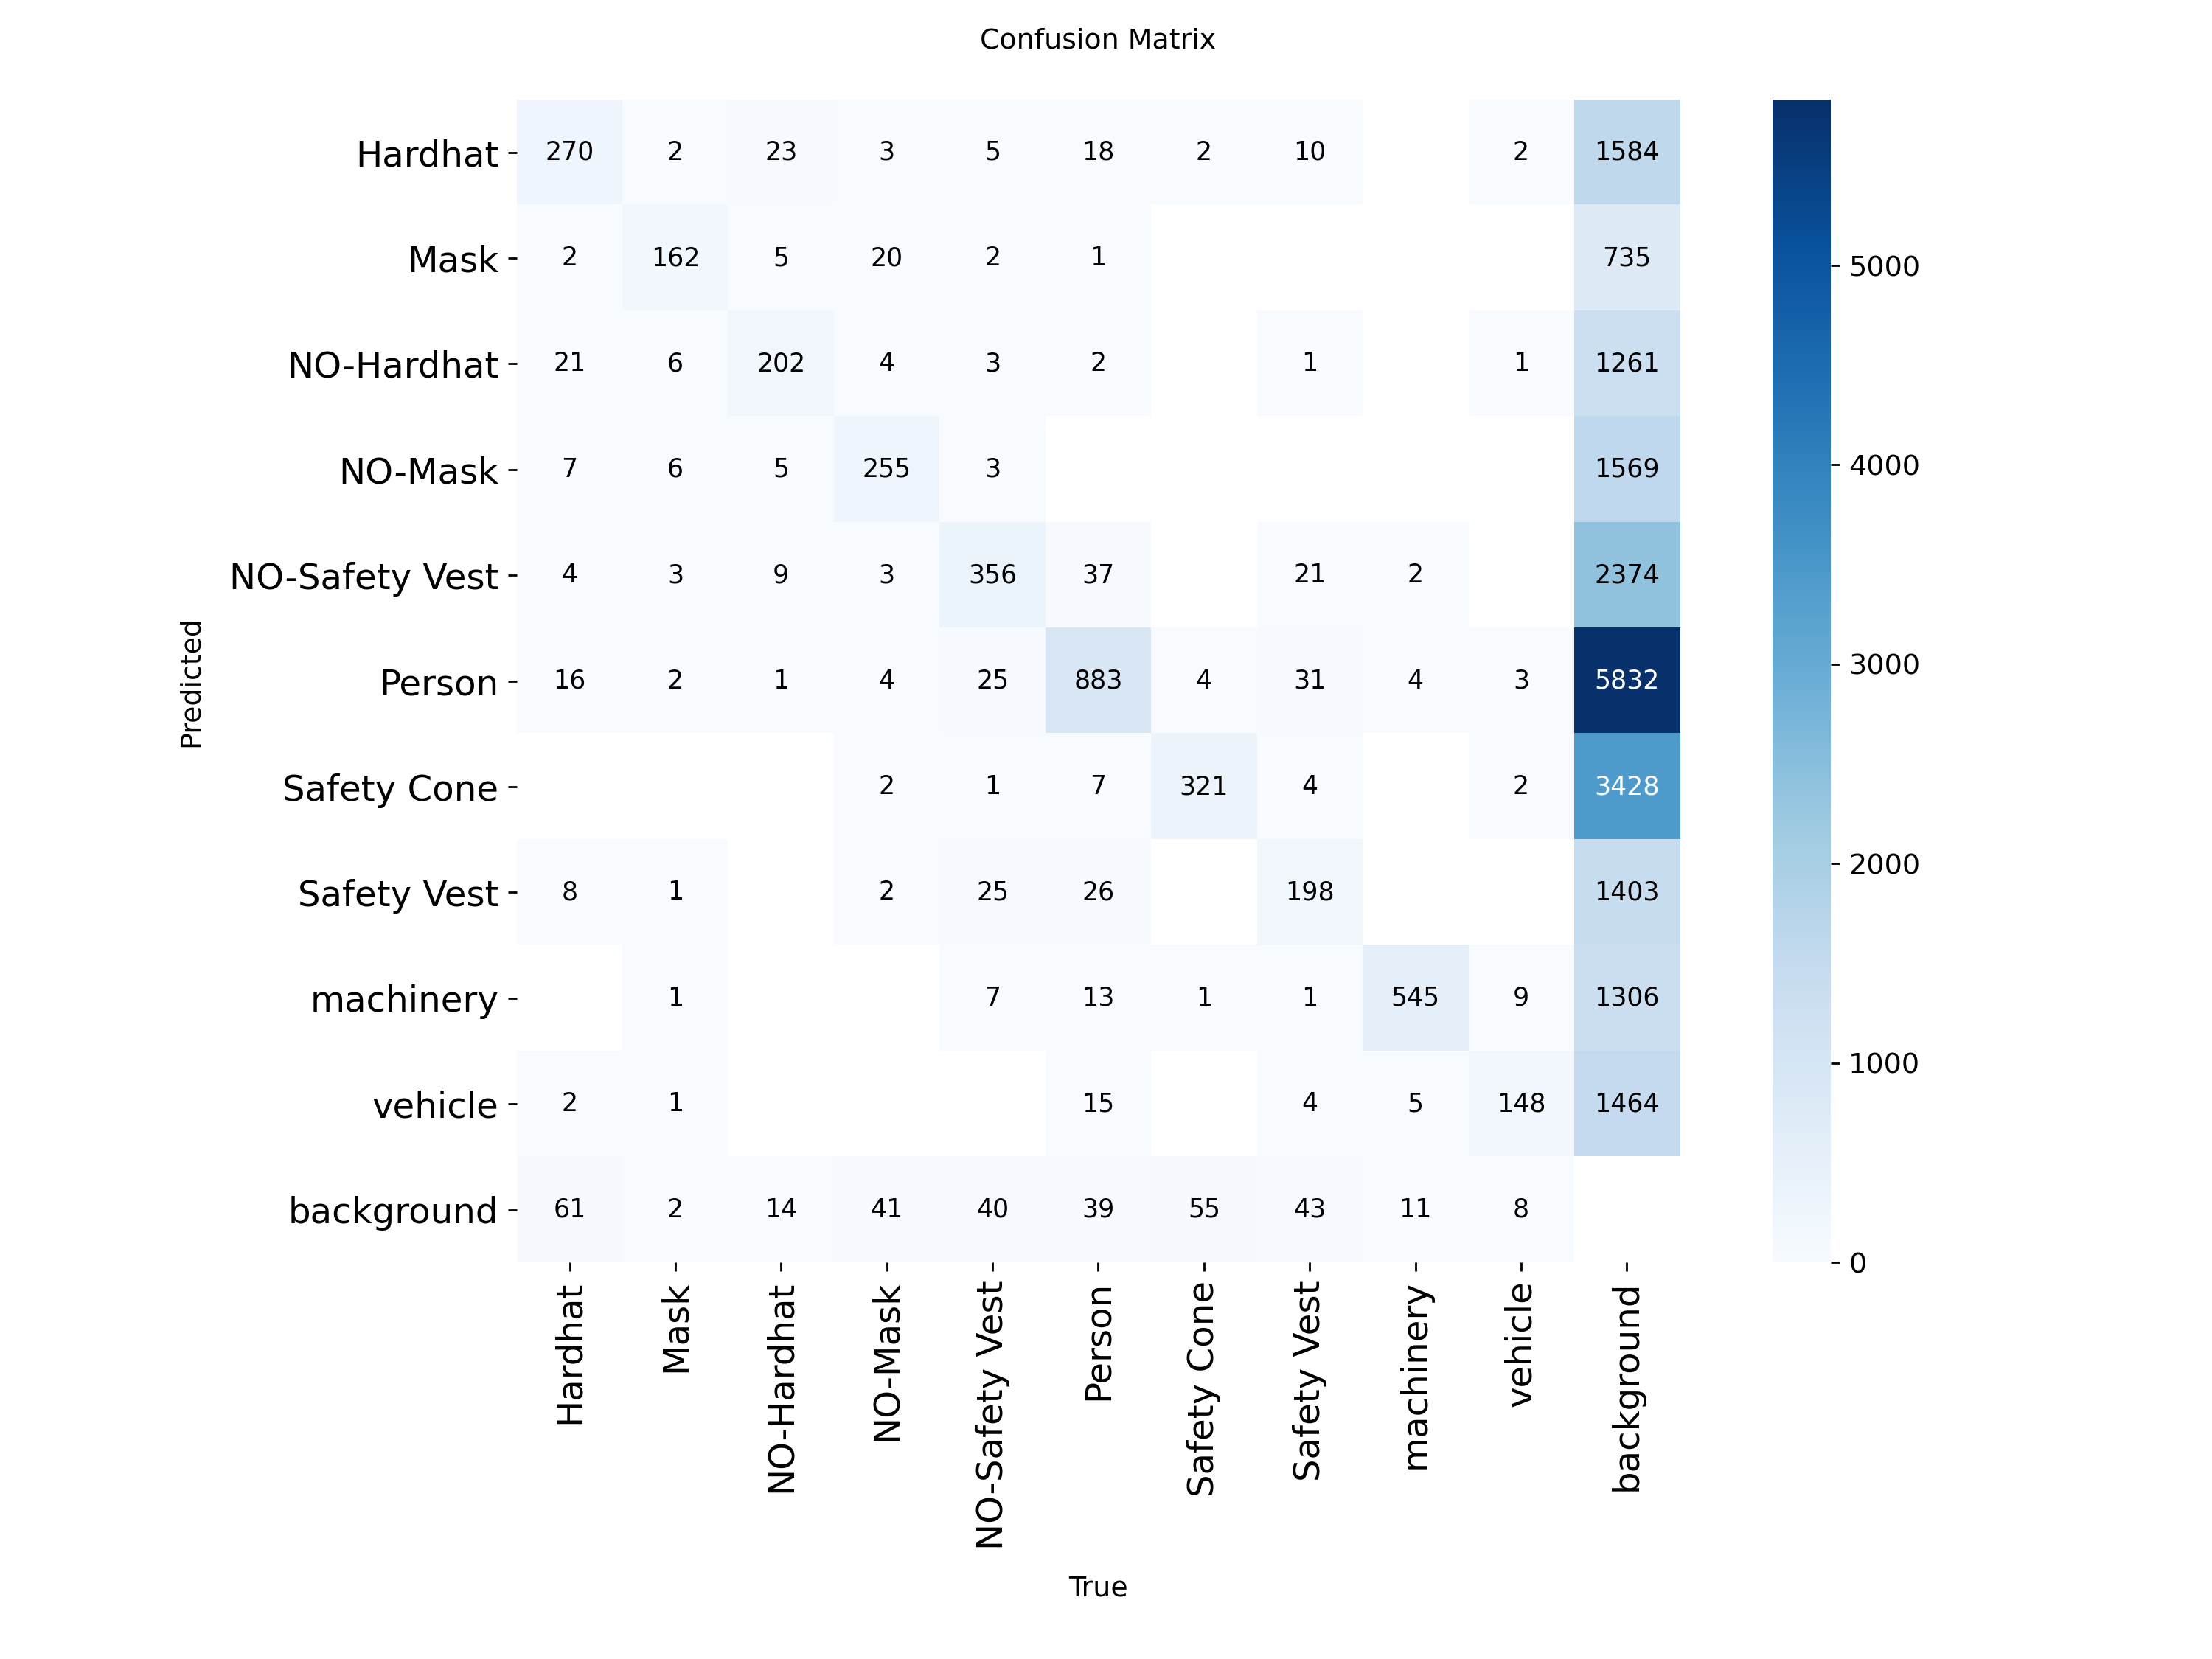
\includegraphics[width=\linewidth]{eval_test_confusion_matrix.png}\caption{Counts}\end{subfigure}\hfill
\begin{subfigure}{0.49\linewidth}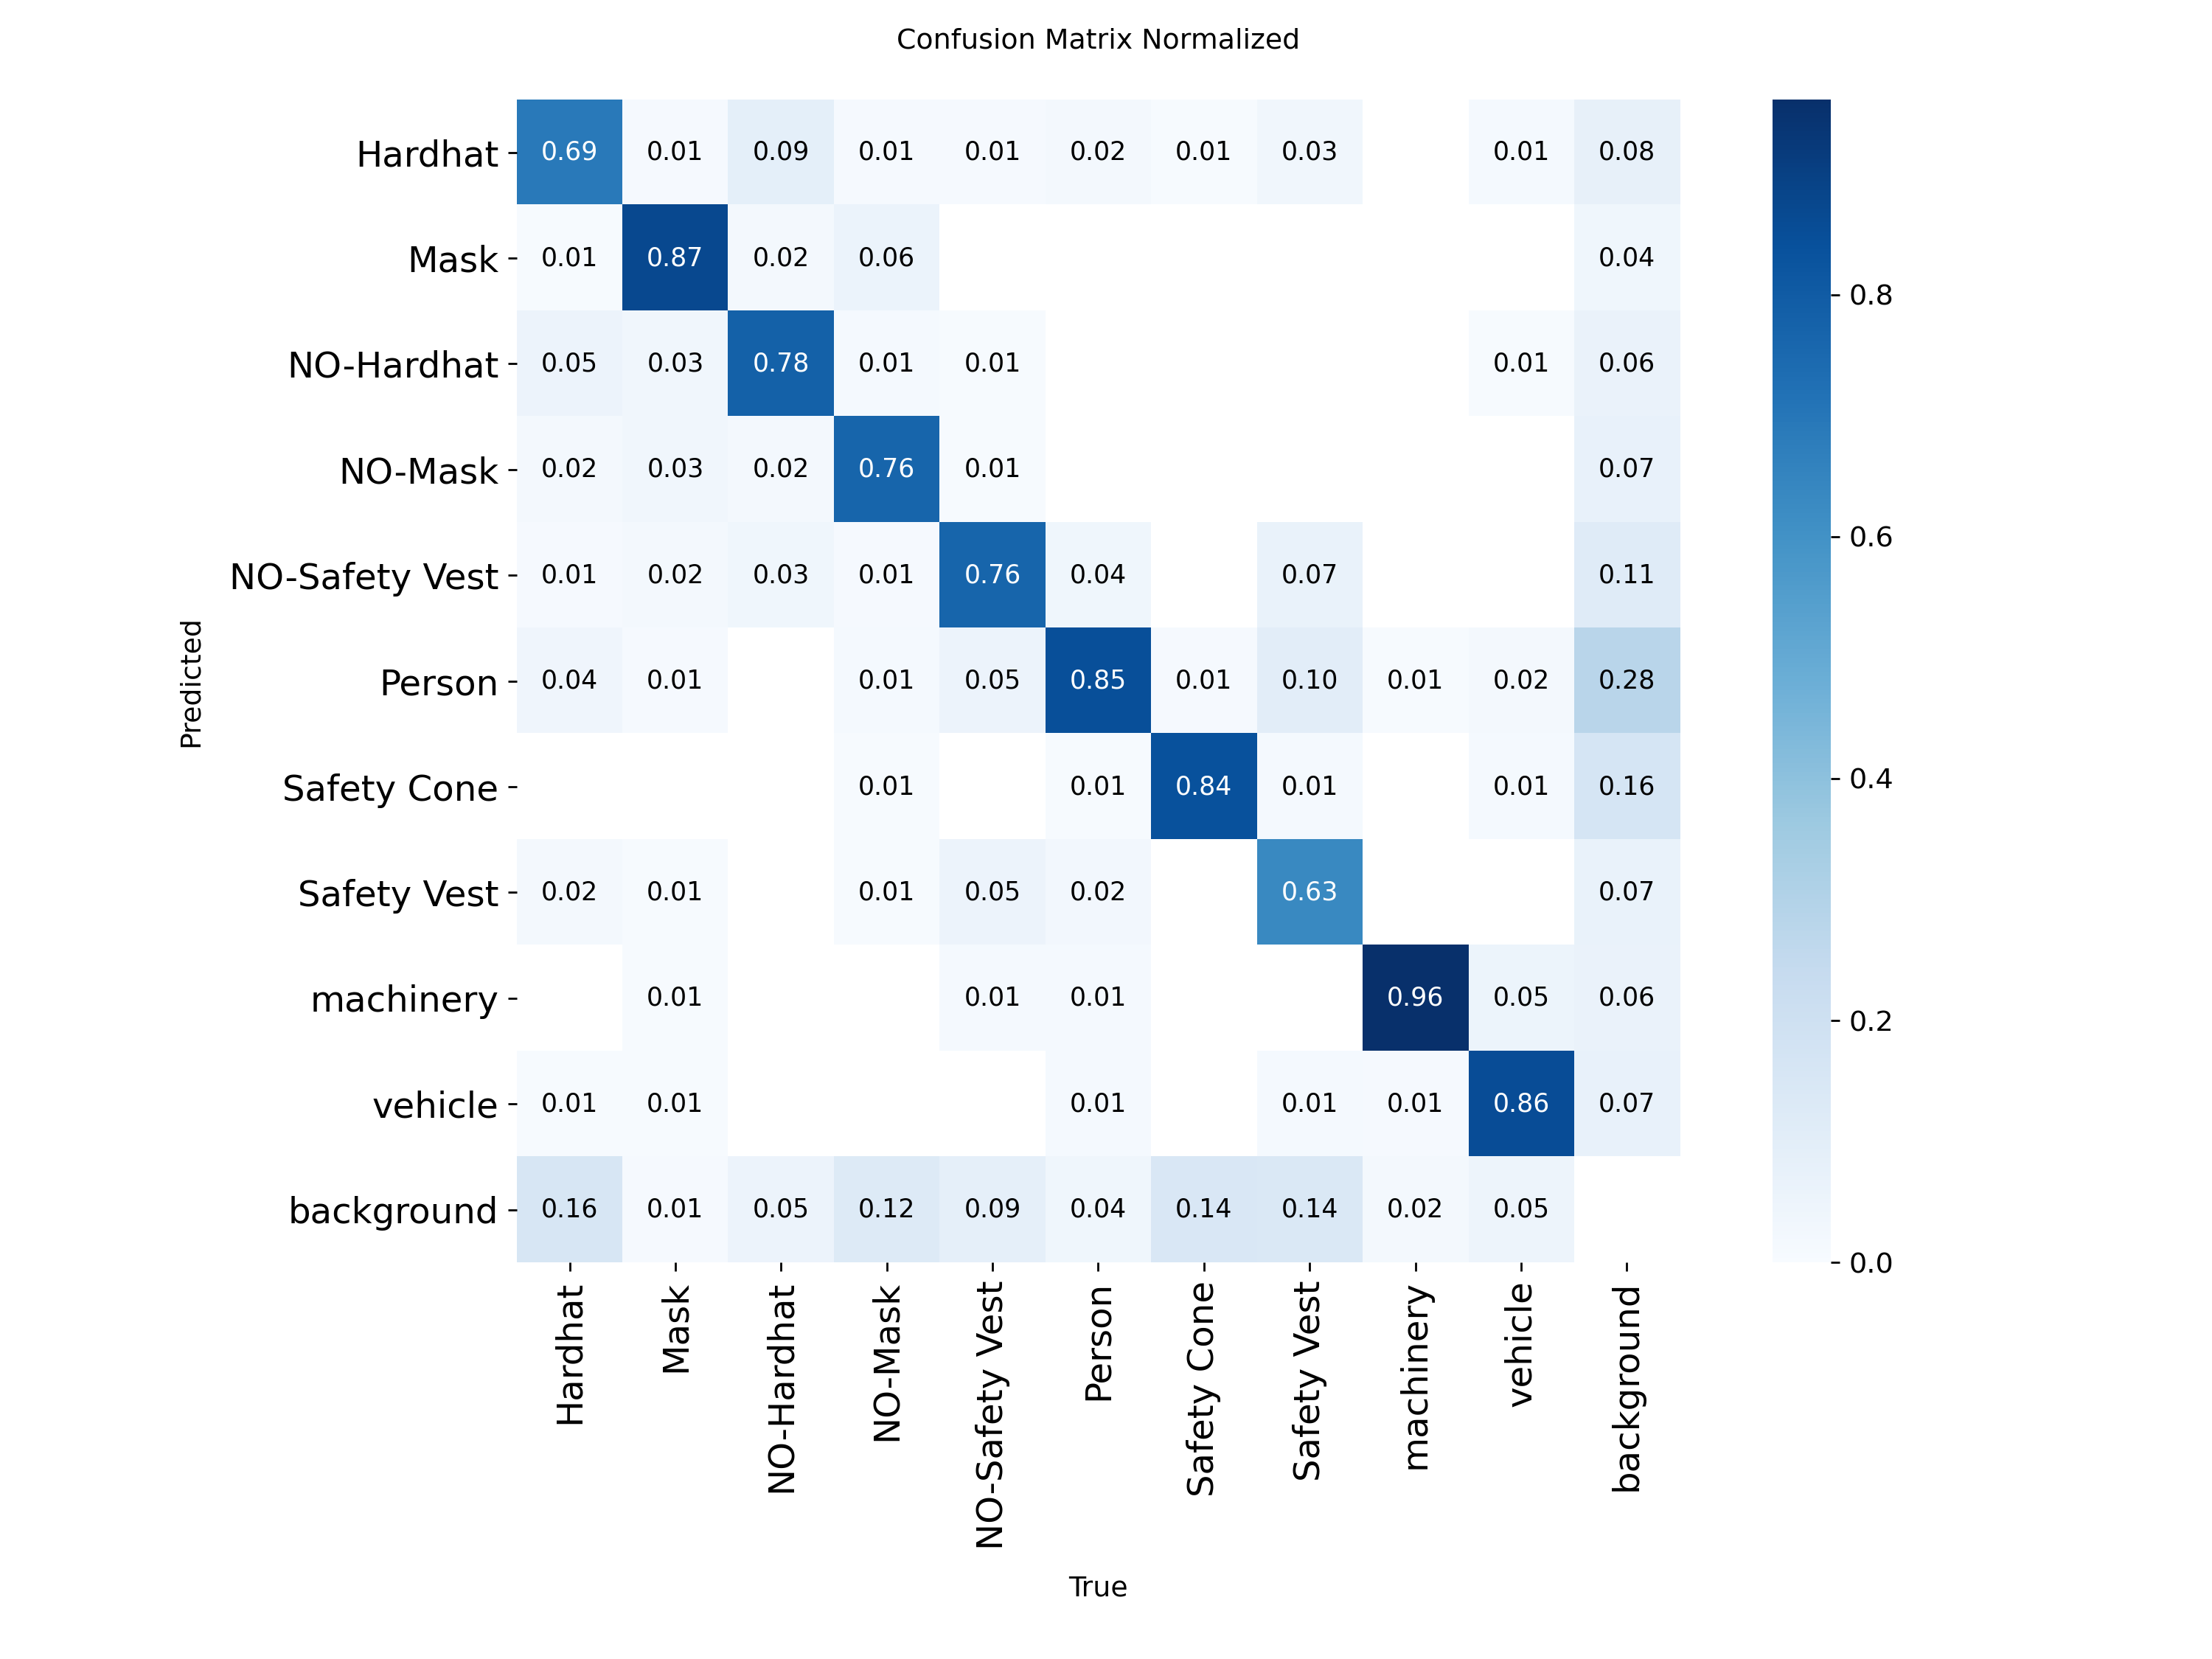
\includegraphics[width=\linewidth]{eval_test_confusion_matrix_normalized.png}\caption{Normalised by true class}\end{subfigure}
\caption{Confusion matrices on the held-out test split.}
\label{fig:testcm}
\end{figure}

Two swaps matter directly for safety. First, 9\% of true NO-Hardhat boxes are predicted as Hardhat, which turns a violation into an apparent compliance; this is the most consequential error for the incident pipeline. Second, 7\% of true Safety Vest boxes are predicted as NO-Safety Vest, which would raise false alarms. On the background side, 28\% of false positives against background are predicted as Person and 16\% as Safety Cone. The temporal filter in \cref{eq:temporal} is meant to suppress such errors when they are transient: a misclassification that appears in fewer than five consecutive frames raises no incident. Errors that persist across frames, such as a NO-Hardhat worker consistently labelled as Hardhat, are not corrected by the filter.

\Cref{fig:samples} shows predictions on six test images chosen with a fixed seed. Workers, hardhats, vests and machinery are localised at several scales. Several dataset images are themselves composites of four photographs, as the examples show.

\begin{figure}[htbp]
\centering
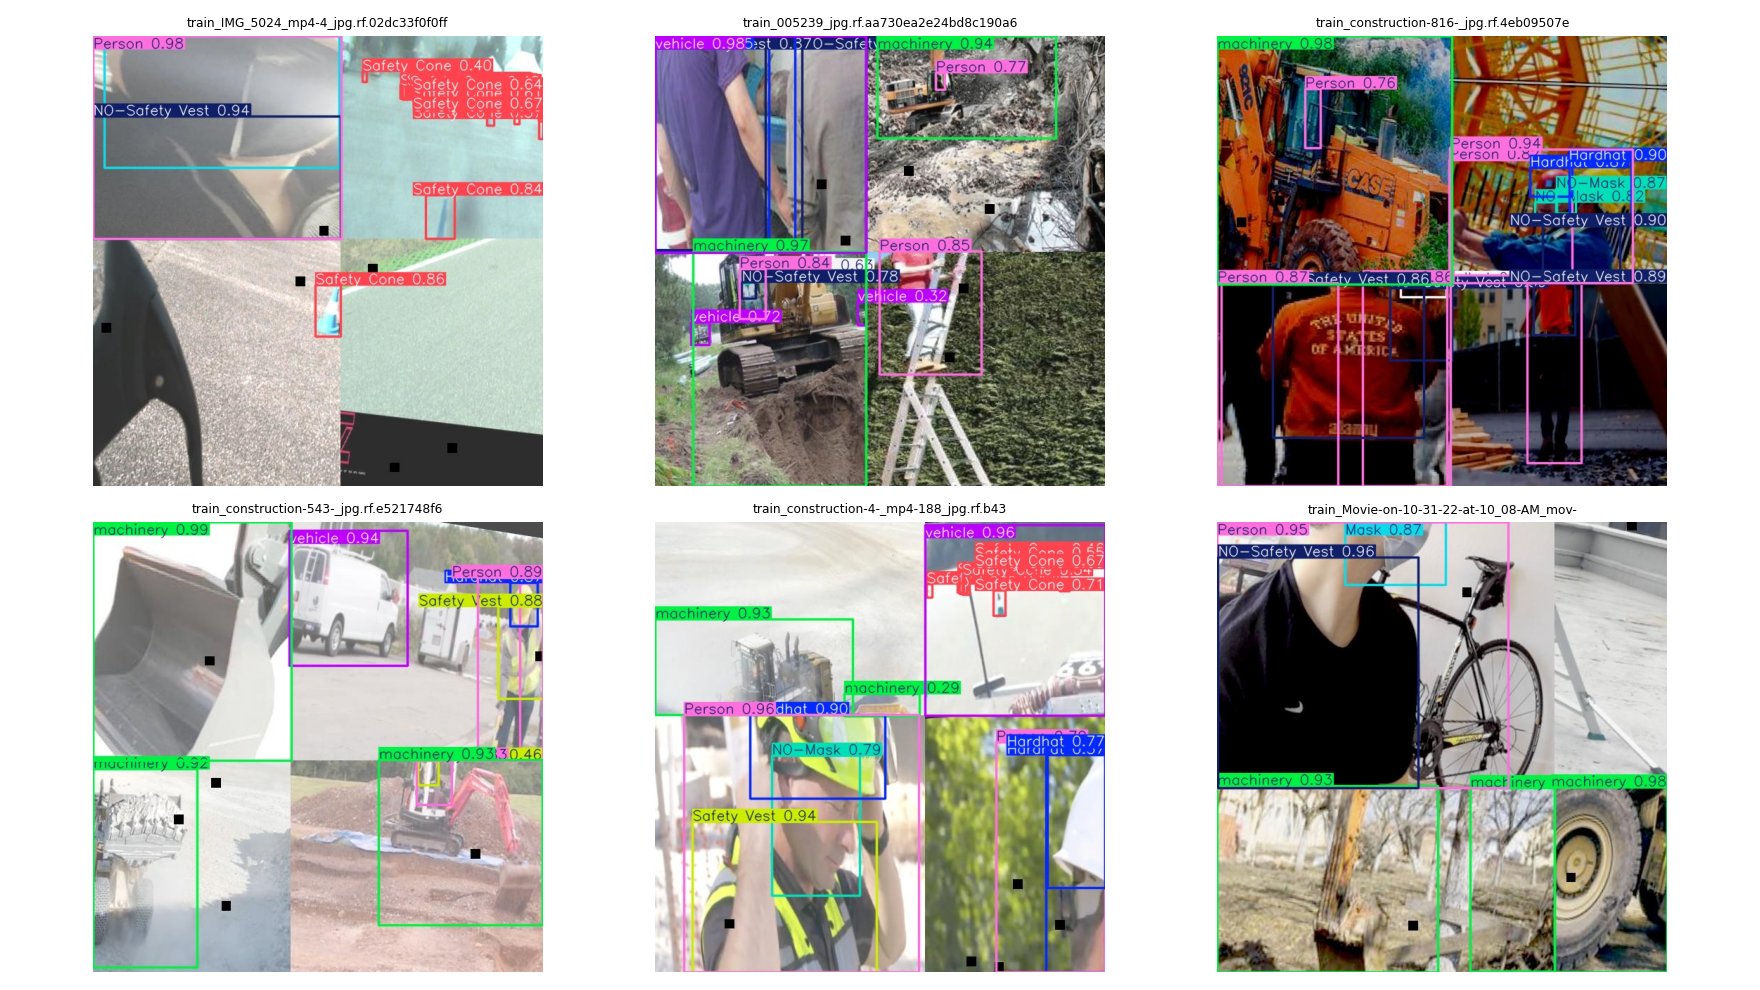
\includegraphics[width=\linewidth,height=0.4\textheight,keepaspectratio]{sample_predictions.png}
\caption{Predicted boxes on six test images selected with seed 42.}
\label{fig:samples}
\end{figure}

\subsection{Comparison with prior work}

Direct numerical comparison with earlier studies is not possible because they use different datasets, class sets and splits. The base study \cite{ferdous2022ppe} reported an average mAP of 89.84\% for YOLOX-m on its eight-class CHVG dataset of 1,699 images, while this work reports an mAP@0.5 of 0.8659 on a different ten-class dataset of 2,801 images that includes explicit violation classes and site-context classes. The two results are of a similar order, but the difference cannot be attributed to the detector alone. What the present work adds is the path from detections to incidents: explicit violation classes, a compliance rule, temporal confirmation for video and a working interface, which detection-only studies do not evaluate.

\subsection{Deployment}

The trained weights are served by a FastAPI backend that exposes endpoints for image analysis, asynchronous video jobs with progress reporting, incident listing, session metrics, threshold configuration and model reload, and a React dashboard presents the results. The model was also exported to ONNX (opset 17, 80.5 MB) with an output tensor of shape $1 \times 14 \times 8400$, four box values and ten class scores for each of 8,400 candidate locations, for runtimes other than PyTorch. The complete notebook, from data loading to export, took 44.88 min, of which training took 43.49 min.

\section{Conclusion and future work}
\label{sec:conclusion}

This paper presented a PPE compliance monitoring system built around a YOLO11m detector fine-tuned for ten construction-site classes. Trained for 75 epochs within a 0.70 h budget on two T4 GPUs, the detector reaches an mAP@0.5 of 0.8659 and an mAP@0.5:0.95 of 0.6158 on a held-out test split at 31.3 ms per image, with closely matching validation results. Test-time augmentation did not help and nearly tripled latency. The error analysis shows that small and thin objects (safety cones, vests and hardhats) account for most missed detections, and that confusing NO-Hardhat with Hardhat is the most safety-critical error. A five-frame temporal confirmation filter and a compliance rule turn detections into incidents, and the system is available as an open-source FastAPI and React application.

The work has several limitations. All metrics come from one training run on one dataset split, without cross-validation or an external test set, so accuracy on other sites, cameras, weather and lighting has not been measured. The compliance score is a frame-level approximation that does not associate PPE items with individual workers. The temporal filter and alert cooldown were set by design rather than tuned on annotated video, and the false-alarm reduction they provide has not been measured. Video jobs are held in memory, so a backend restart loses running jobs, and model inference is guarded by a lock, so concurrent jobs share a single inference stream.

Future work will address these points: associating PPE boxes with person boxes and tracking workers across frames to compute per-worker compliance; evaluating on footage from other sites and under adverse conditions; tuning the temporal window and thresholds on annotated video to quantify false-alarm reduction; targeting the weak classes with higher input resolution or small-object augmentation; and comparing YOLO11 with transformer-based real-time detectors such as RT-DETR \cite{zhao2024rtdetr} on the same split.

\section*{Data and code availability}

The source code, training notebook, trained weights and all result files are available at \url{https://github.com/parthmital/PPE-Compliance-Monitor}. The dataset is publicly available on Kaggle at the address given in \cref{sec:setup}.

\appendix

\section{Additional evaluation plots}
\label{app:plots}

This appendix collects the remaining plots produced by the training and evaluation runs. \Cref{fig:valcurves,fig:valcm} show the curves and confusion matrices of the validation split. \Cref{fig:runresults} shows the per-epoch summary drawn by Ultralytics during training. \Cref{fig:runcurves,fig:runcm} show the curves and confusion matrices from the validation that ran at the end of training, on the same validation split as \cref{fig:valcurves,fig:valcm} but from a separate call. \Cref{fig:ttacurves,fig:ttacm} show the test split evaluated with TTA.

\begin{figure}[htbp]
\centering
\begin{subfigure}{0.49\linewidth}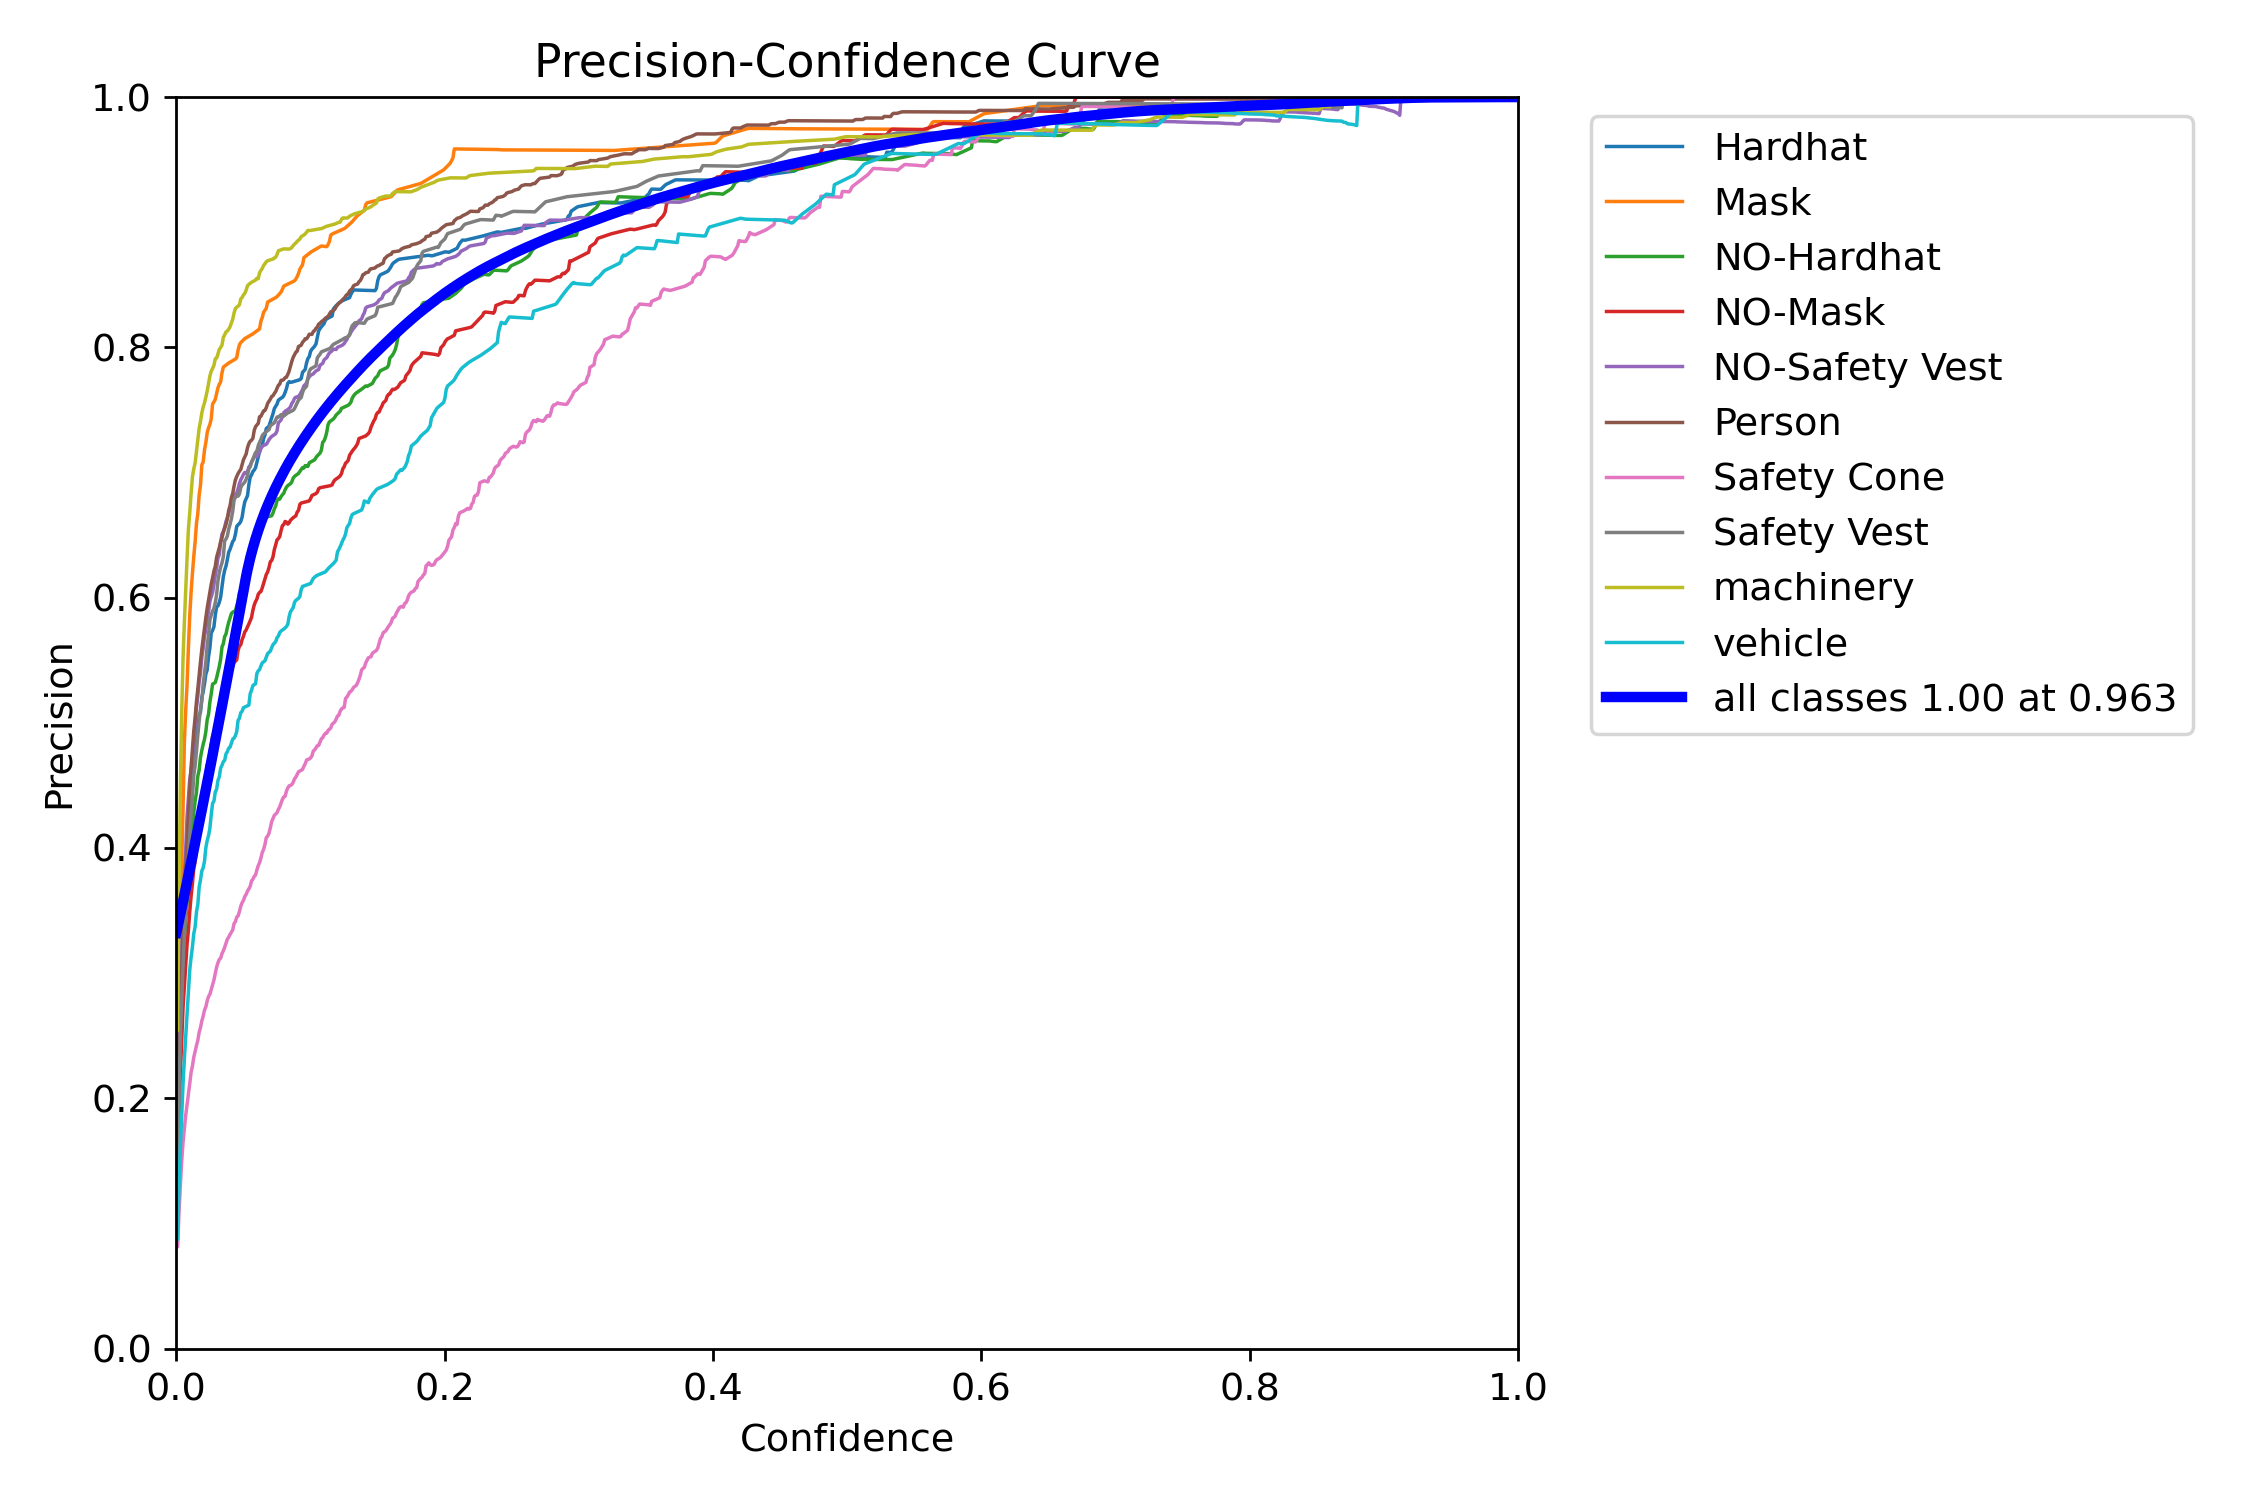
\includegraphics[width=\linewidth]{eval_val_BoxP_curve.png}\caption{Precision}\end{subfigure}\hfill
\begin{subfigure}{0.49\linewidth}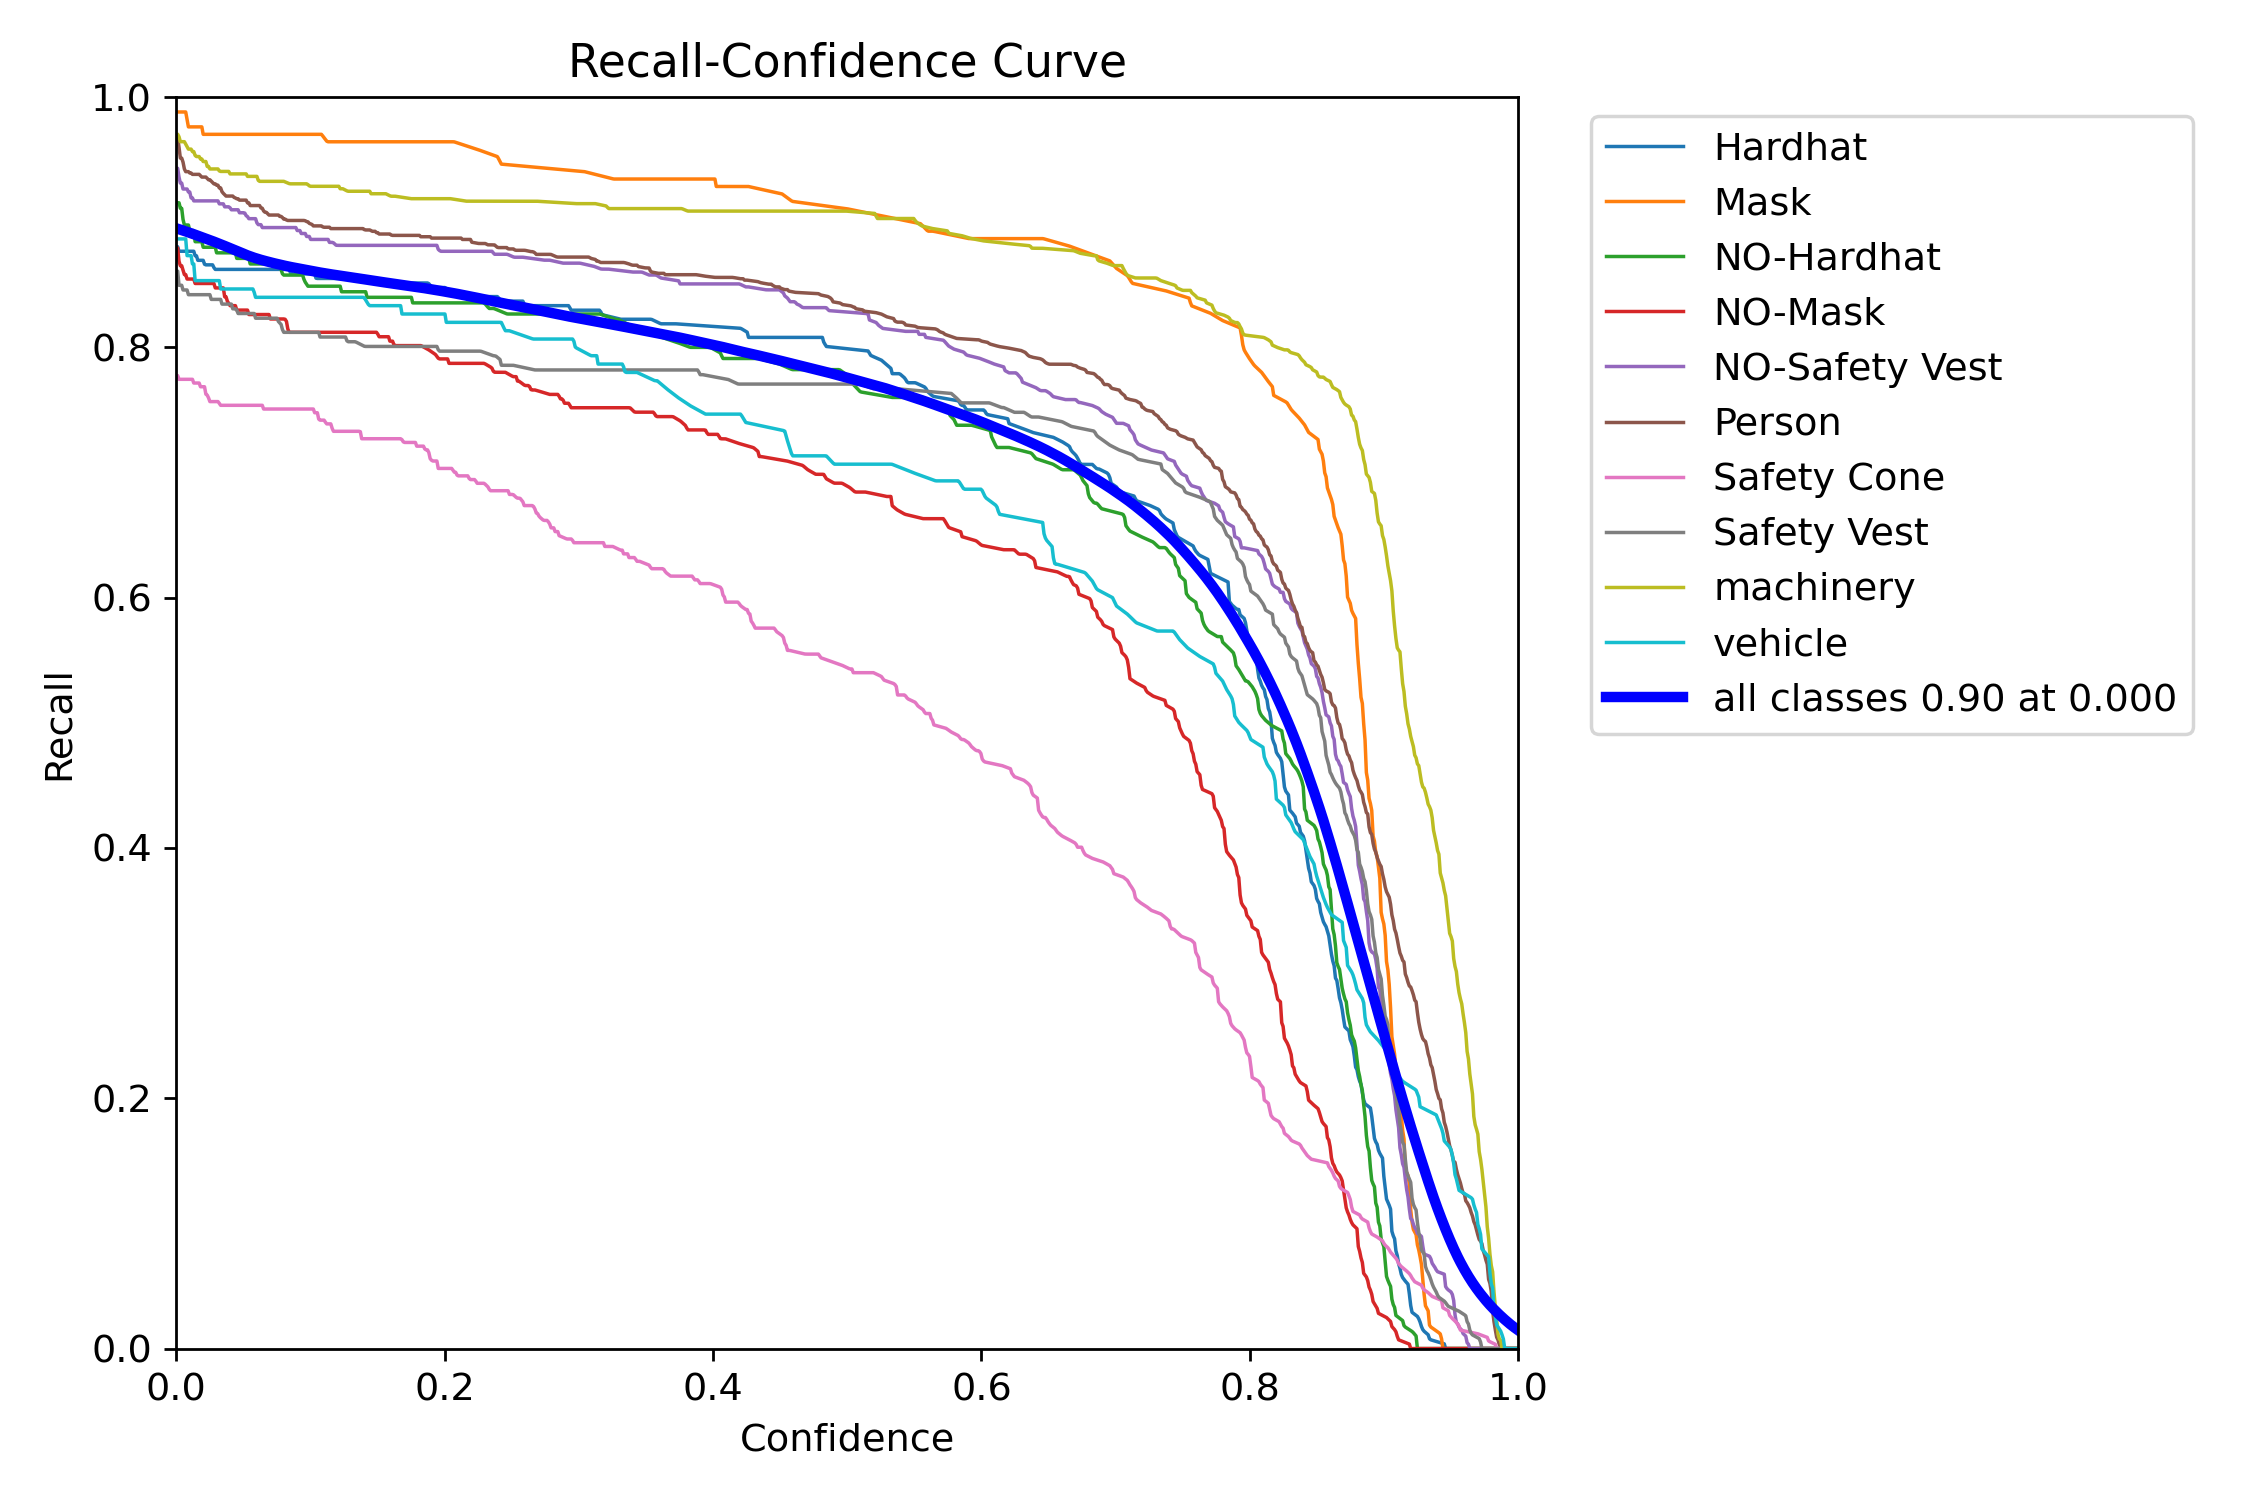
\includegraphics[width=\linewidth]{eval_val_BoxR_curve.png}\caption{Recall}\end{subfigure}\\[2mm]
\begin{subfigure}{0.49\linewidth}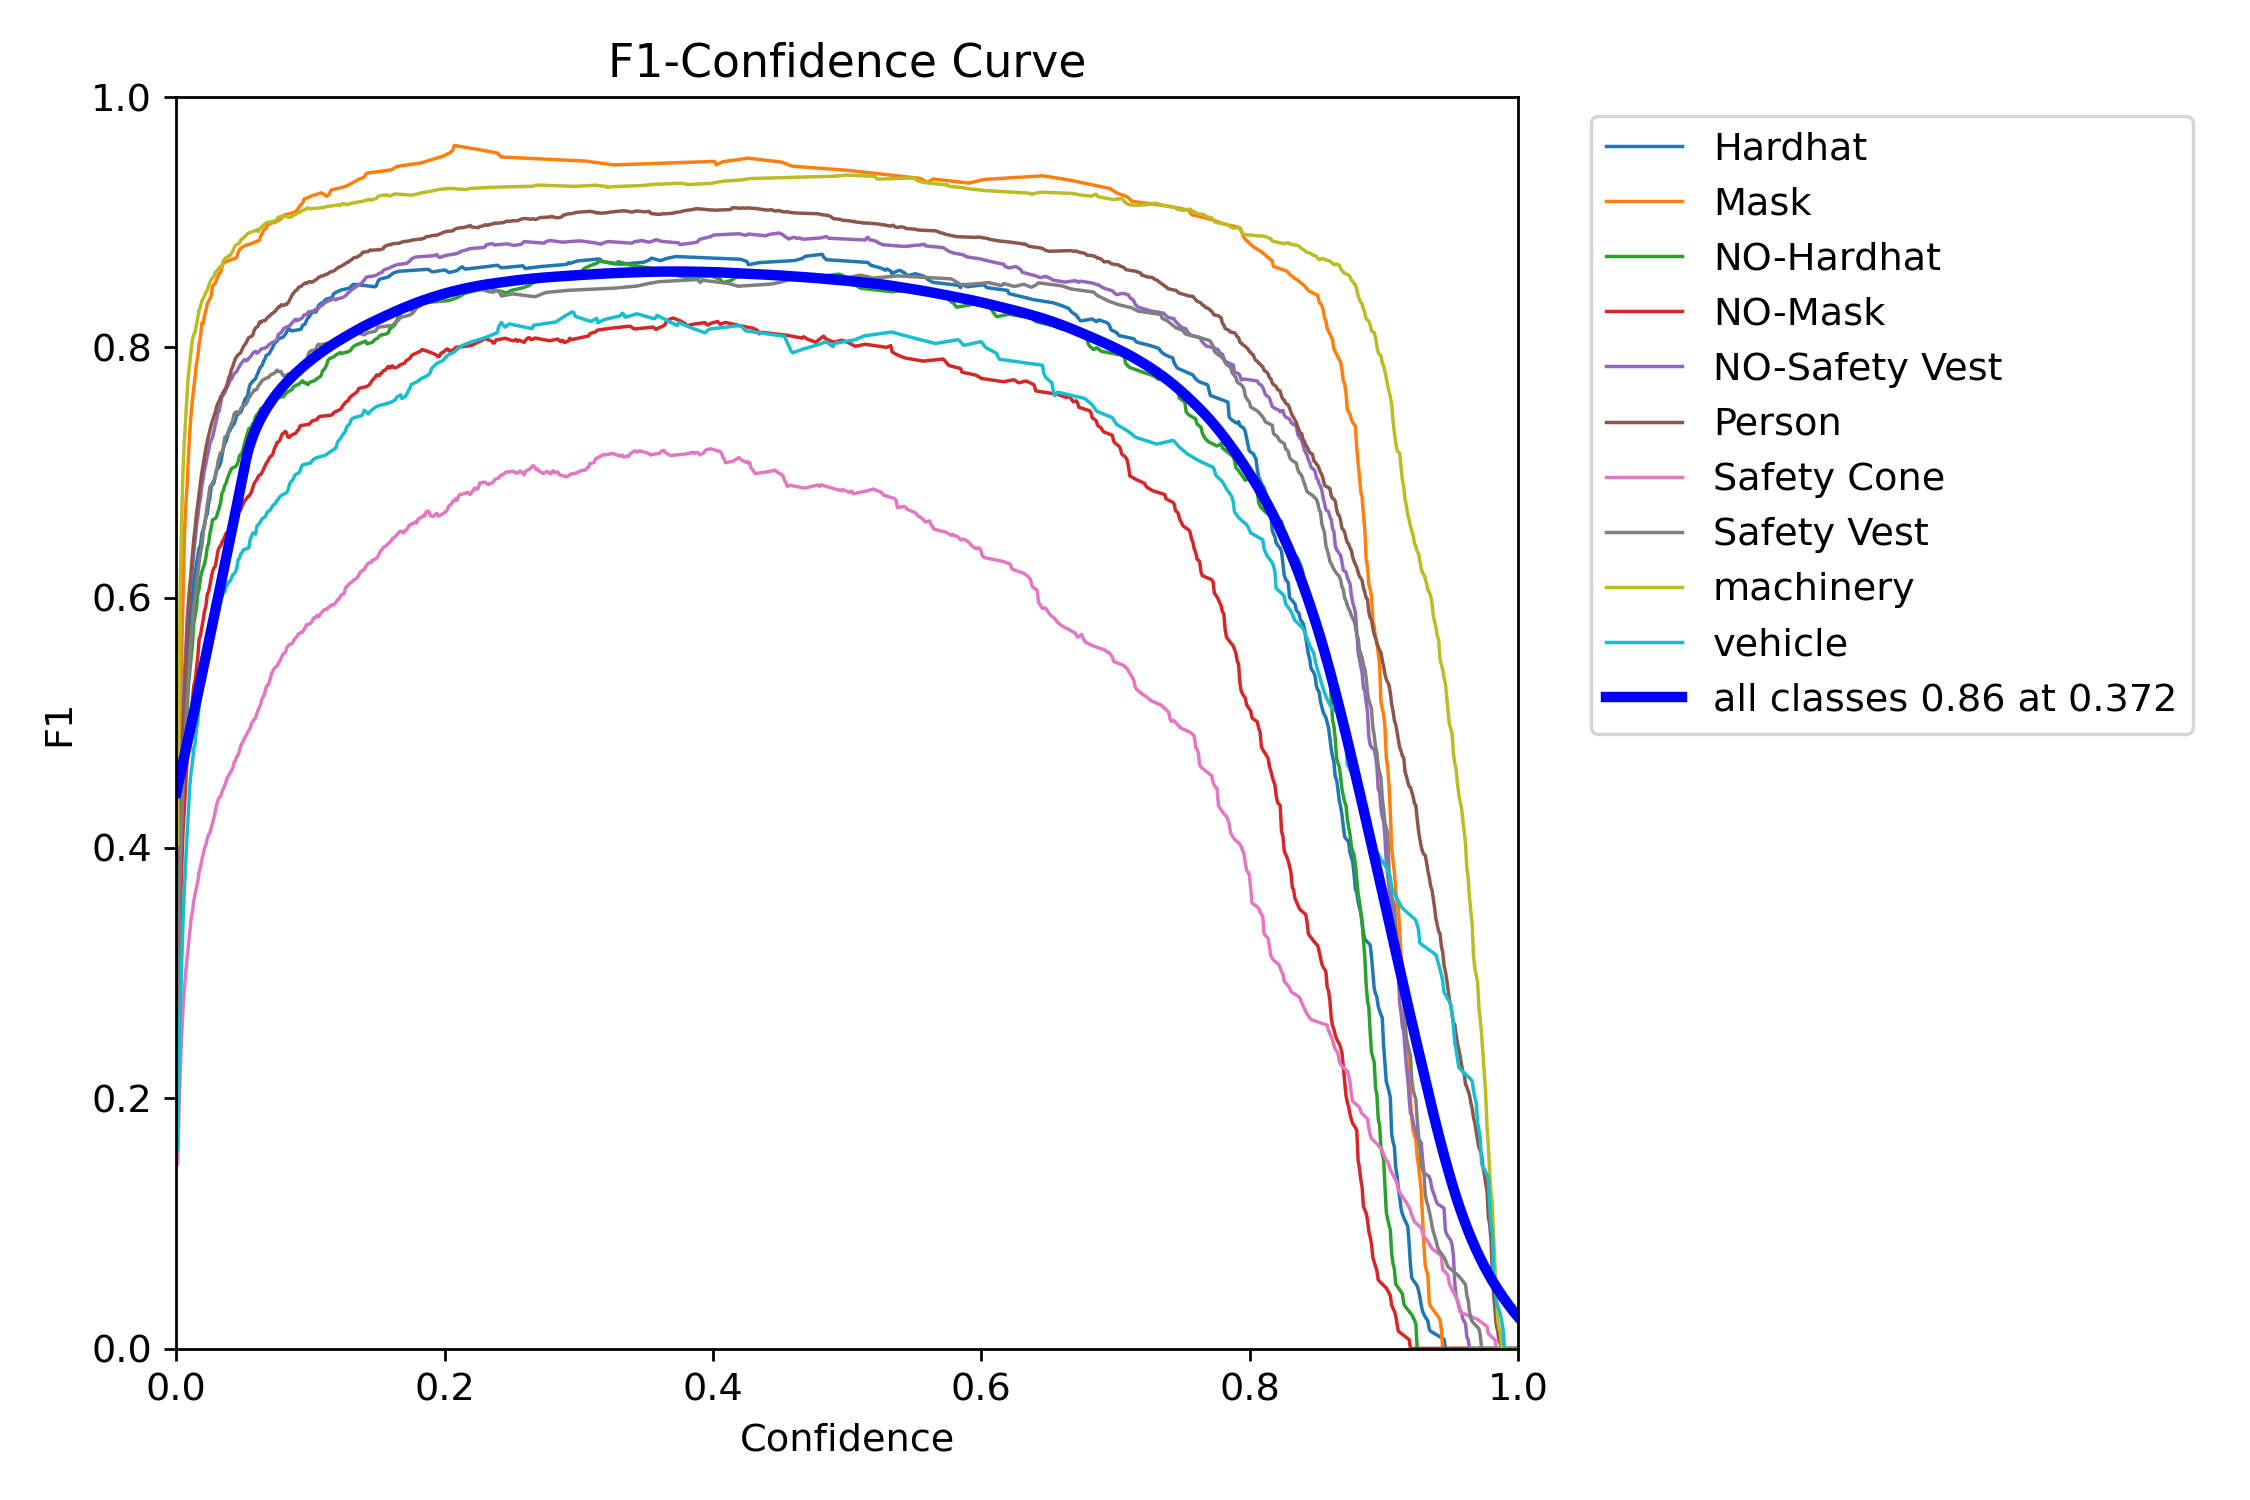
\includegraphics[width=\linewidth]{eval_val_BoxF1_curve.png}\caption{F1}\end{subfigure}\hfill
\begin{subfigure}{0.49\linewidth}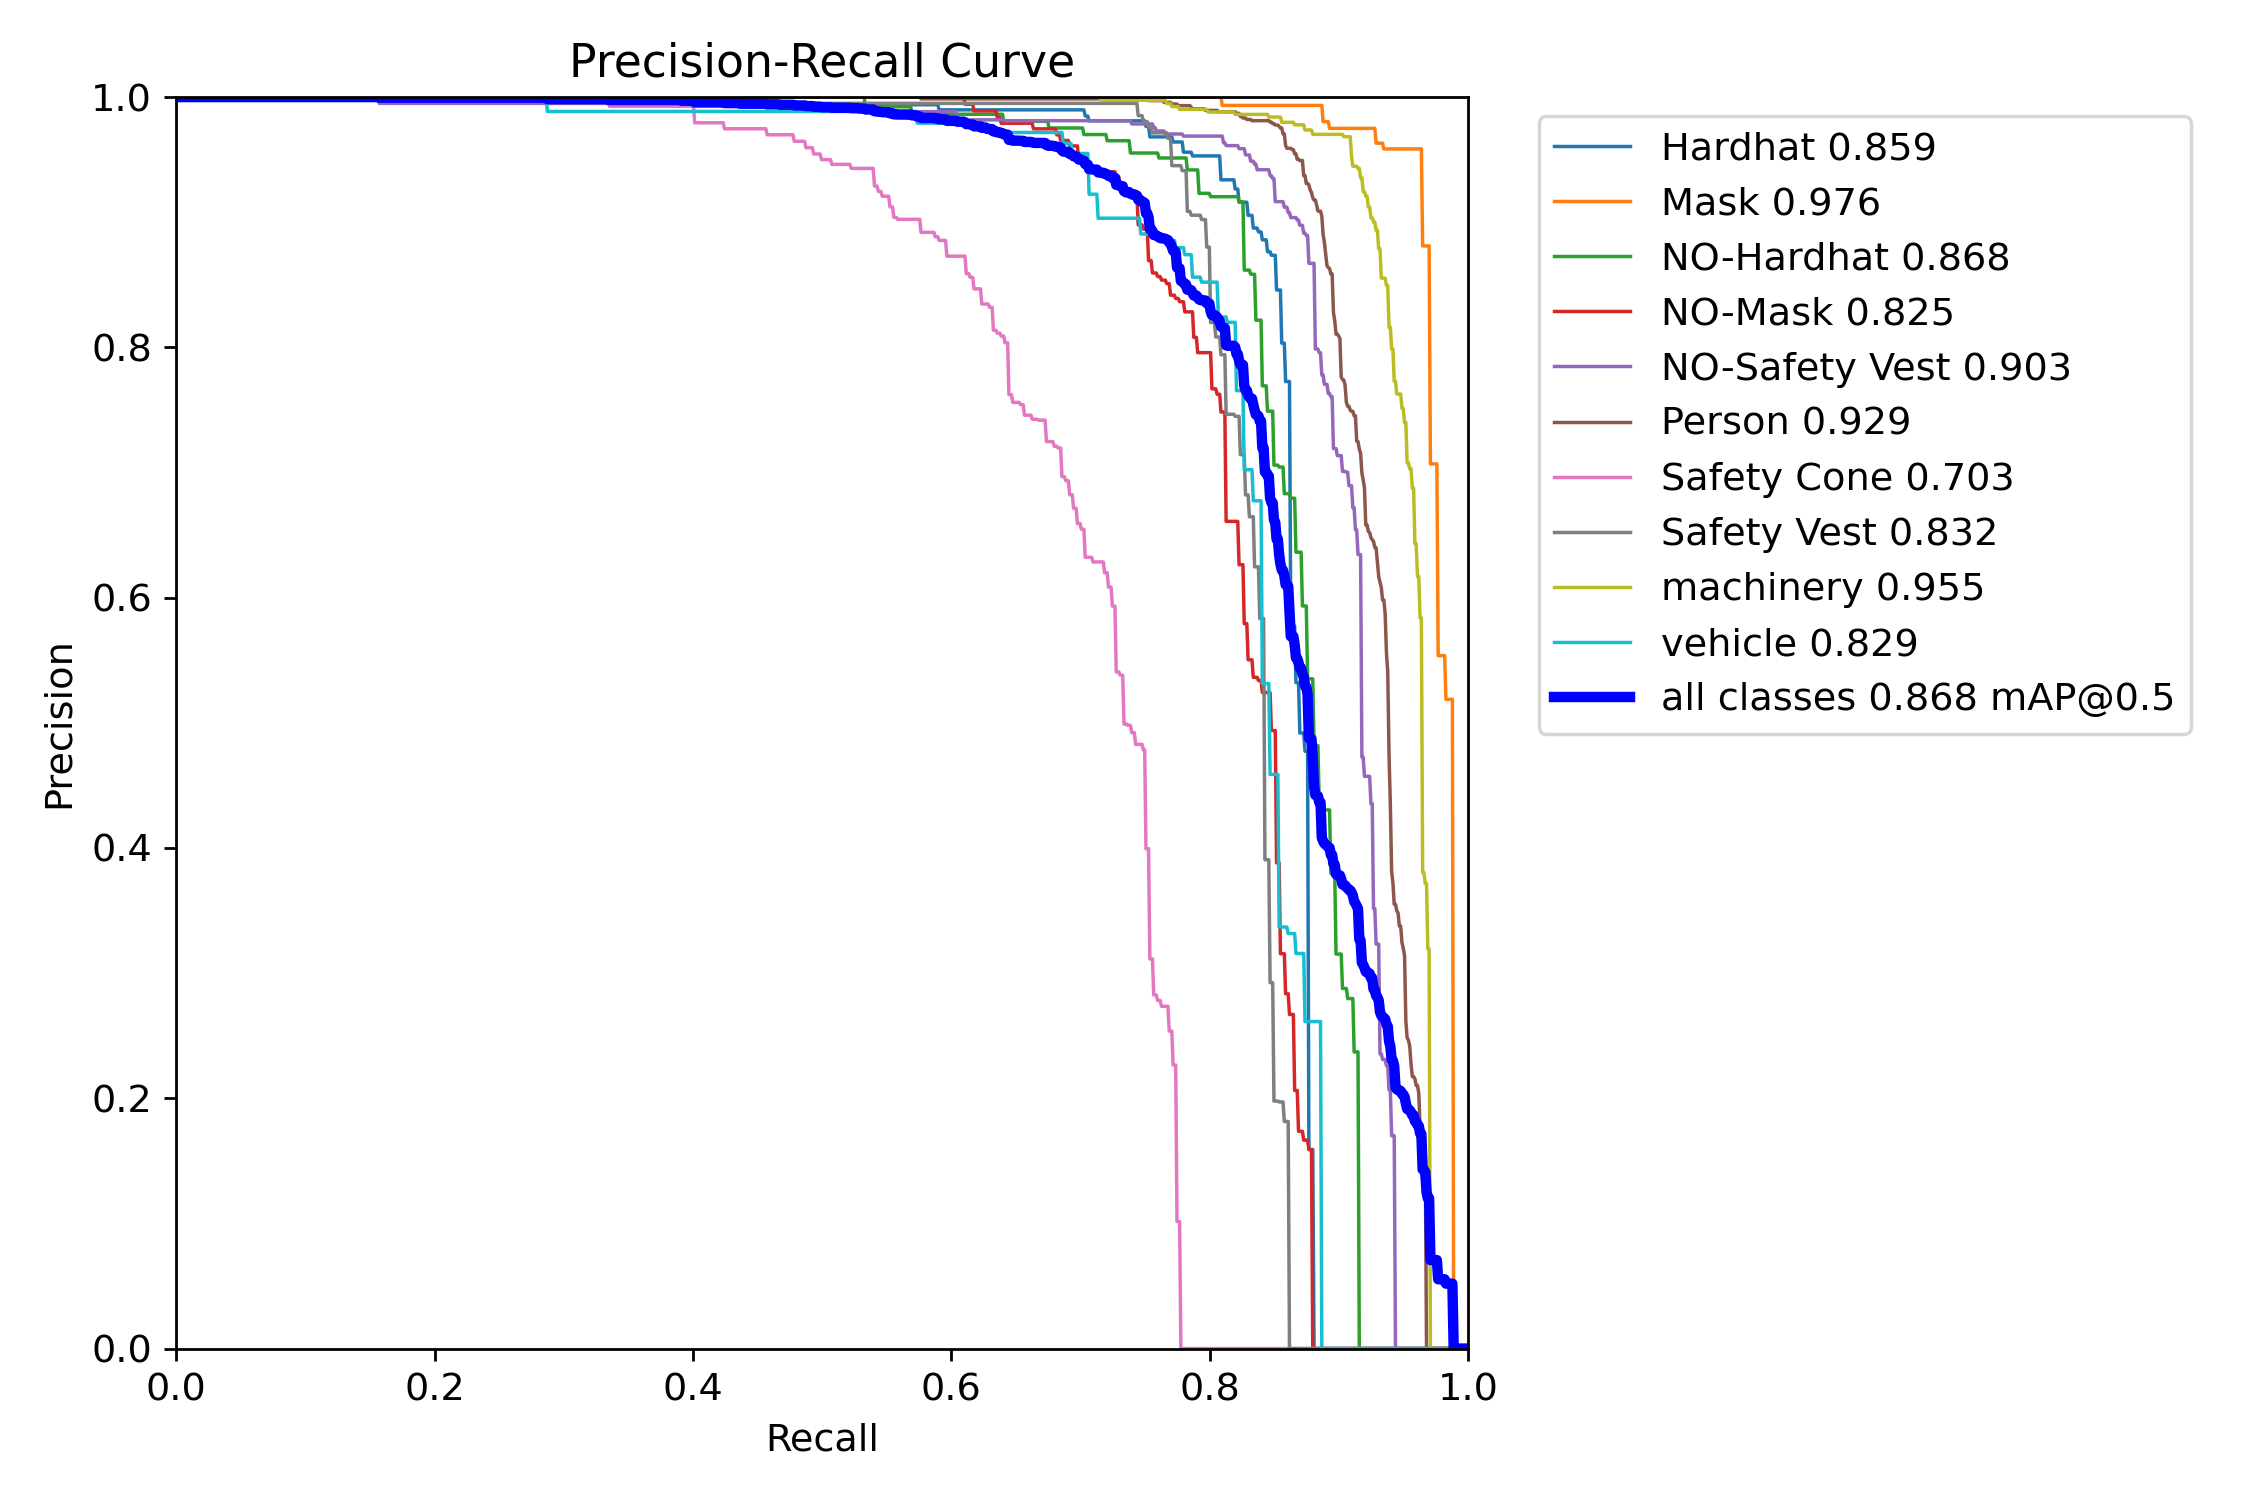
\includegraphics[width=\linewidth]{eval_val_BoxPR_curve.png}\caption{Precision-recall}\end{subfigure}
\caption{Validation split (280 images): precision, recall and F1 against confidence, and the precision-recall curve per class.}
\label{fig:valcurves}
\end{figure}

\begin{figure}[htbp]
\centering
\begin{subfigure}{0.49\linewidth}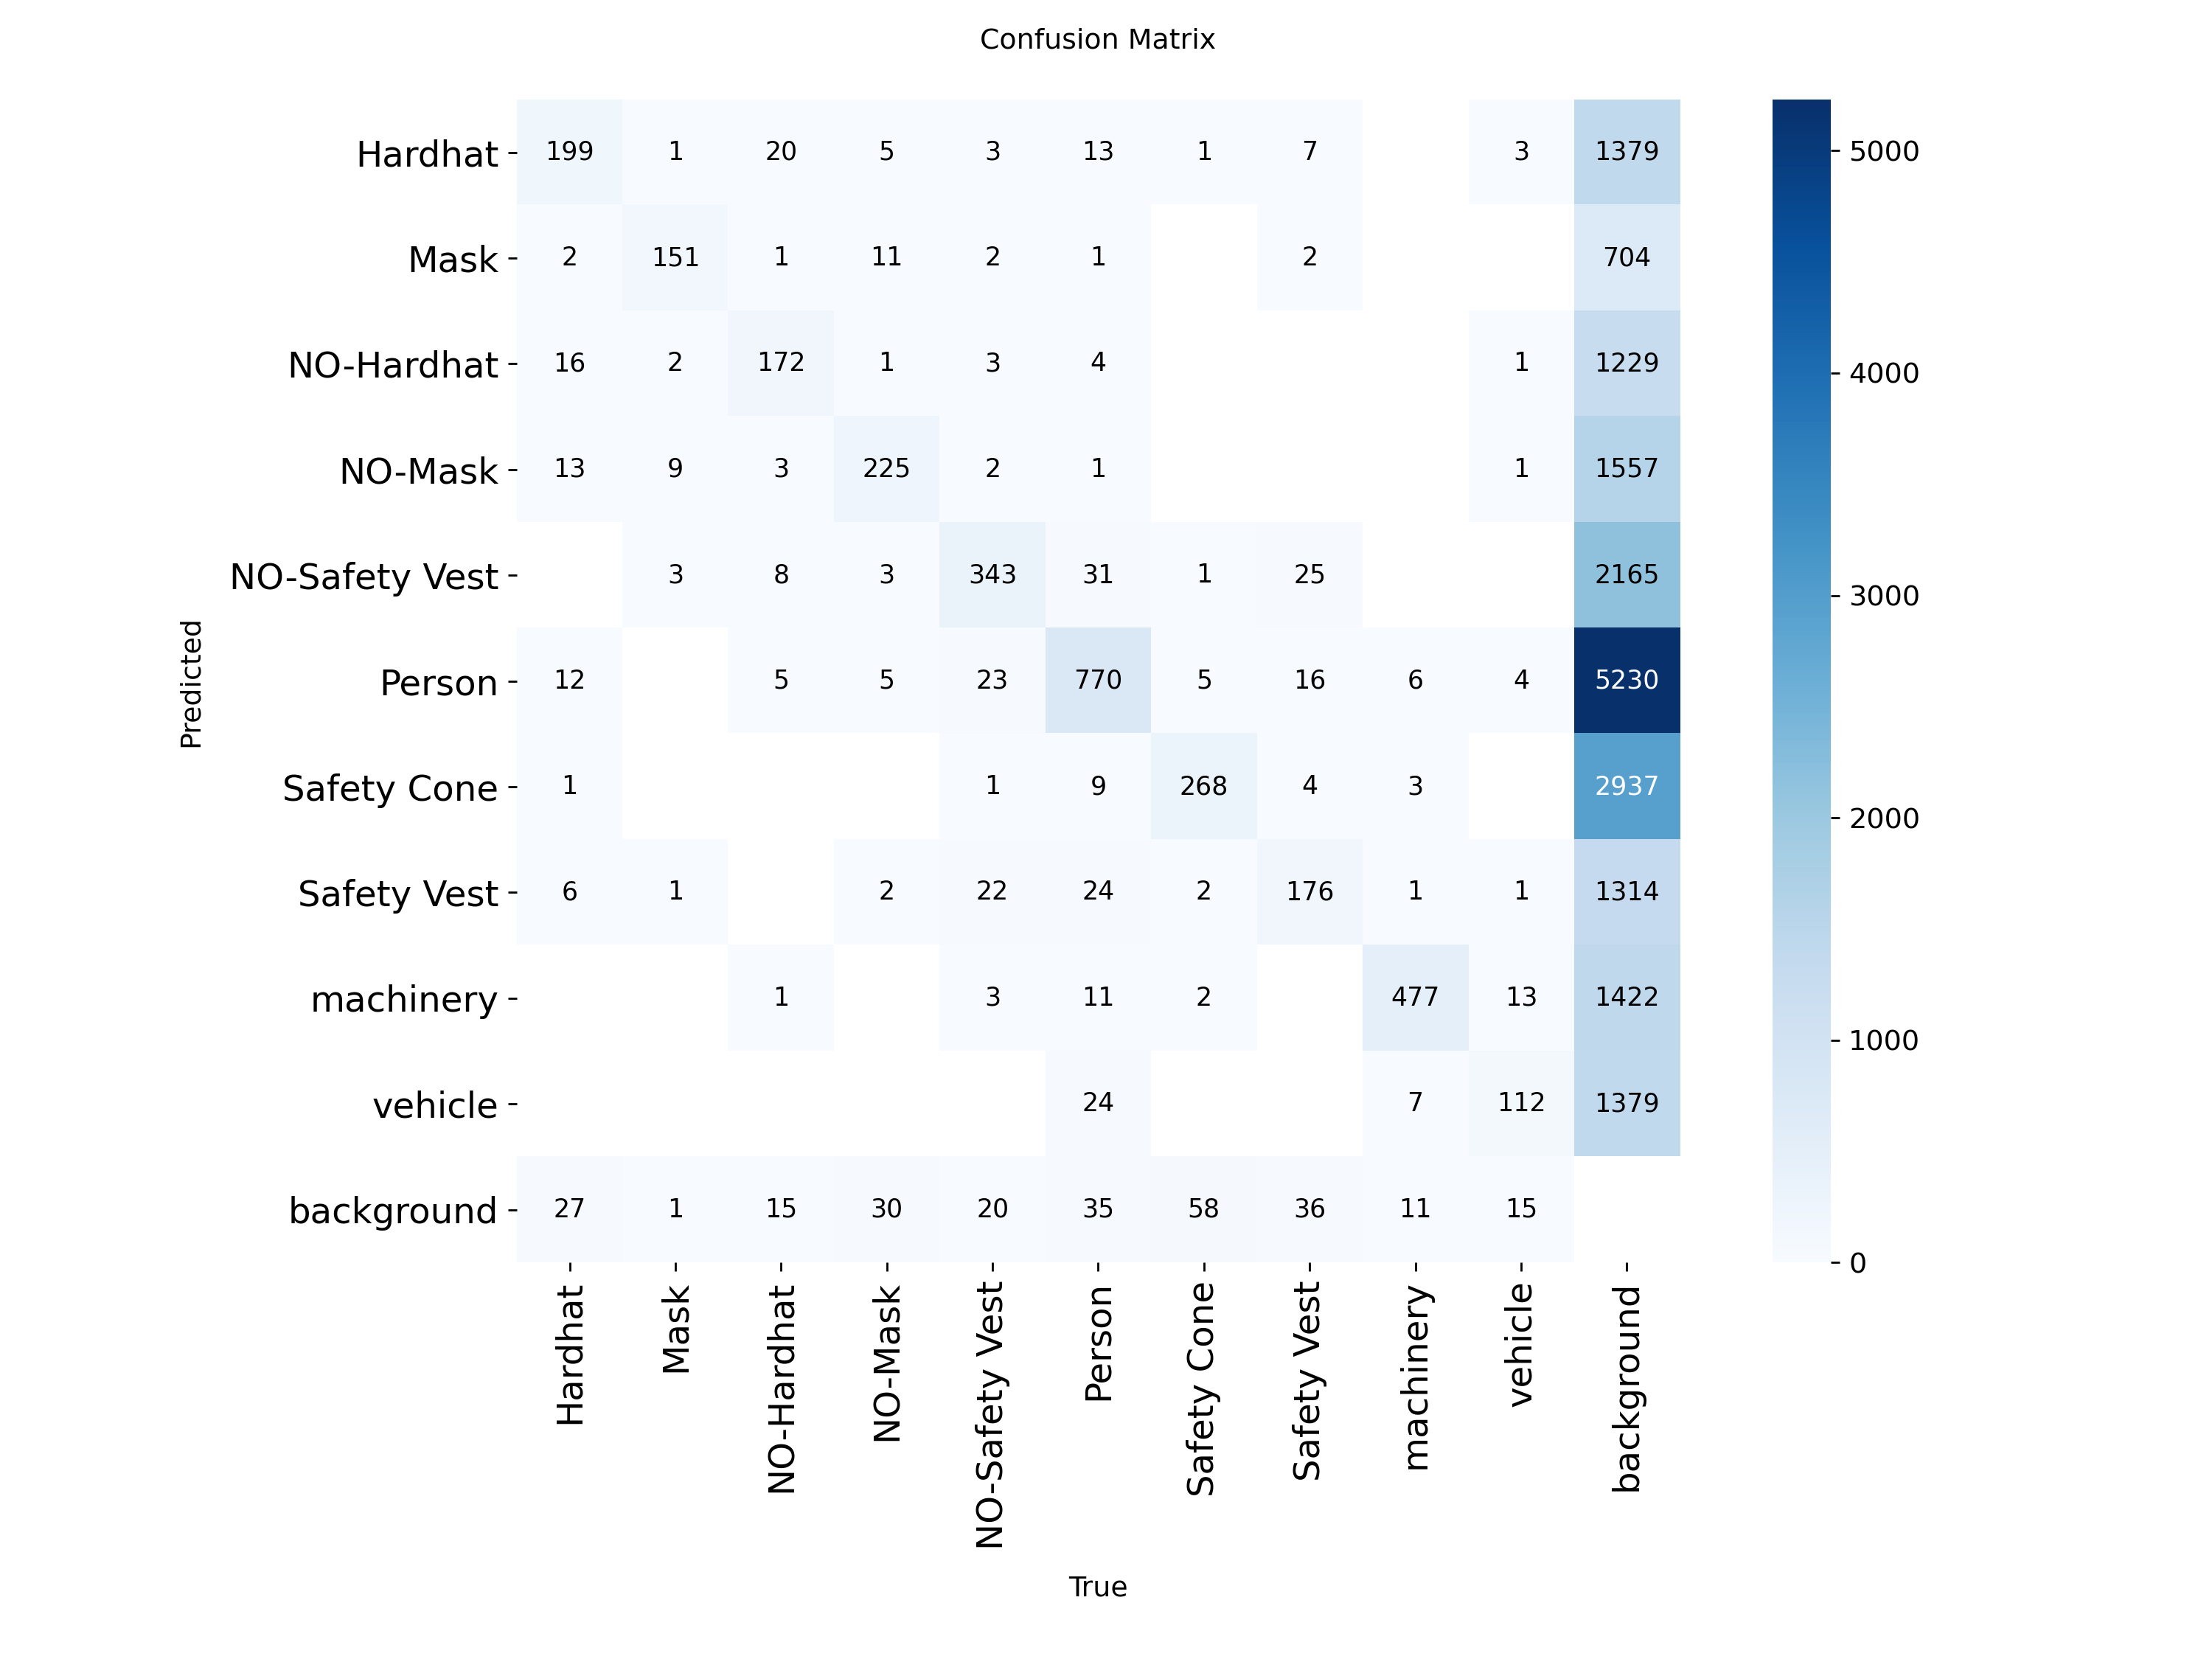
\includegraphics[width=\linewidth]{eval_val_confusion_matrix.png}\caption{Counts}\end{subfigure}\hfill
\begin{subfigure}{0.49\linewidth}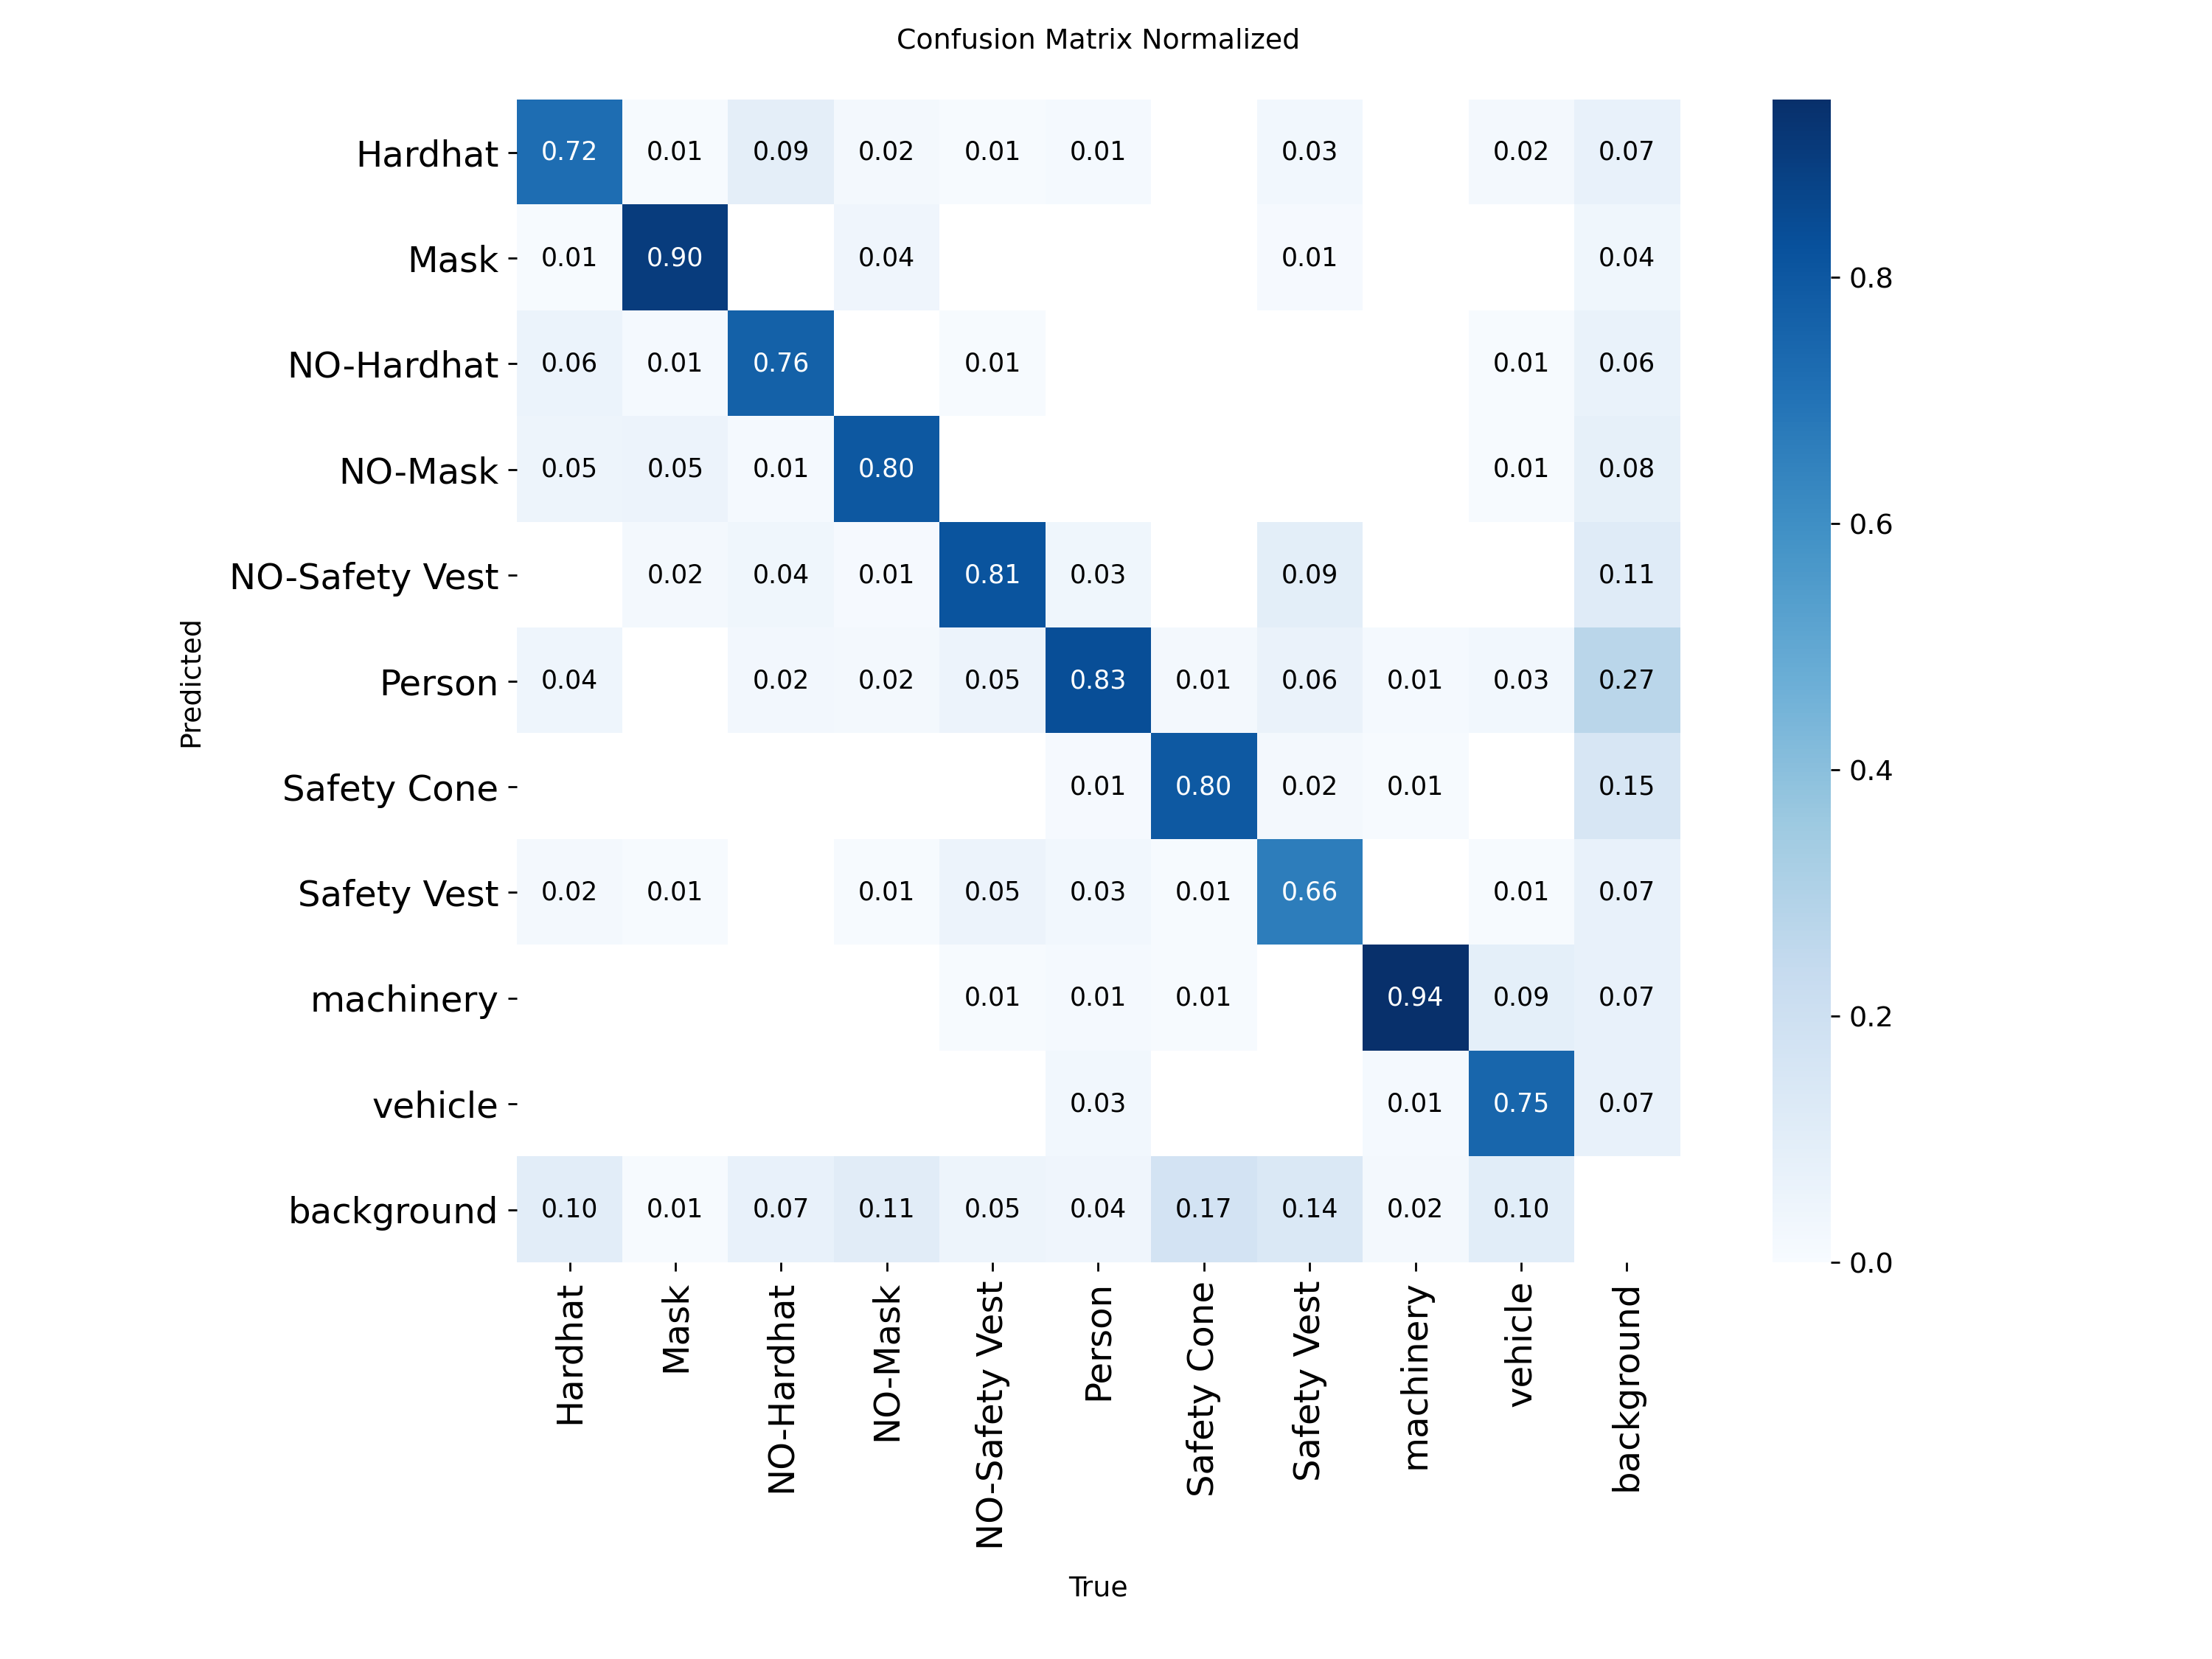
\includegraphics[width=\linewidth]{eval_val_confusion_matrix_normalized.png}\caption{Normalised by true class}\end{subfigure}
\caption{Confusion matrices on the validation split.}
\label{fig:valcm}
\end{figure}

\begin{figure}[htbp]
\centering
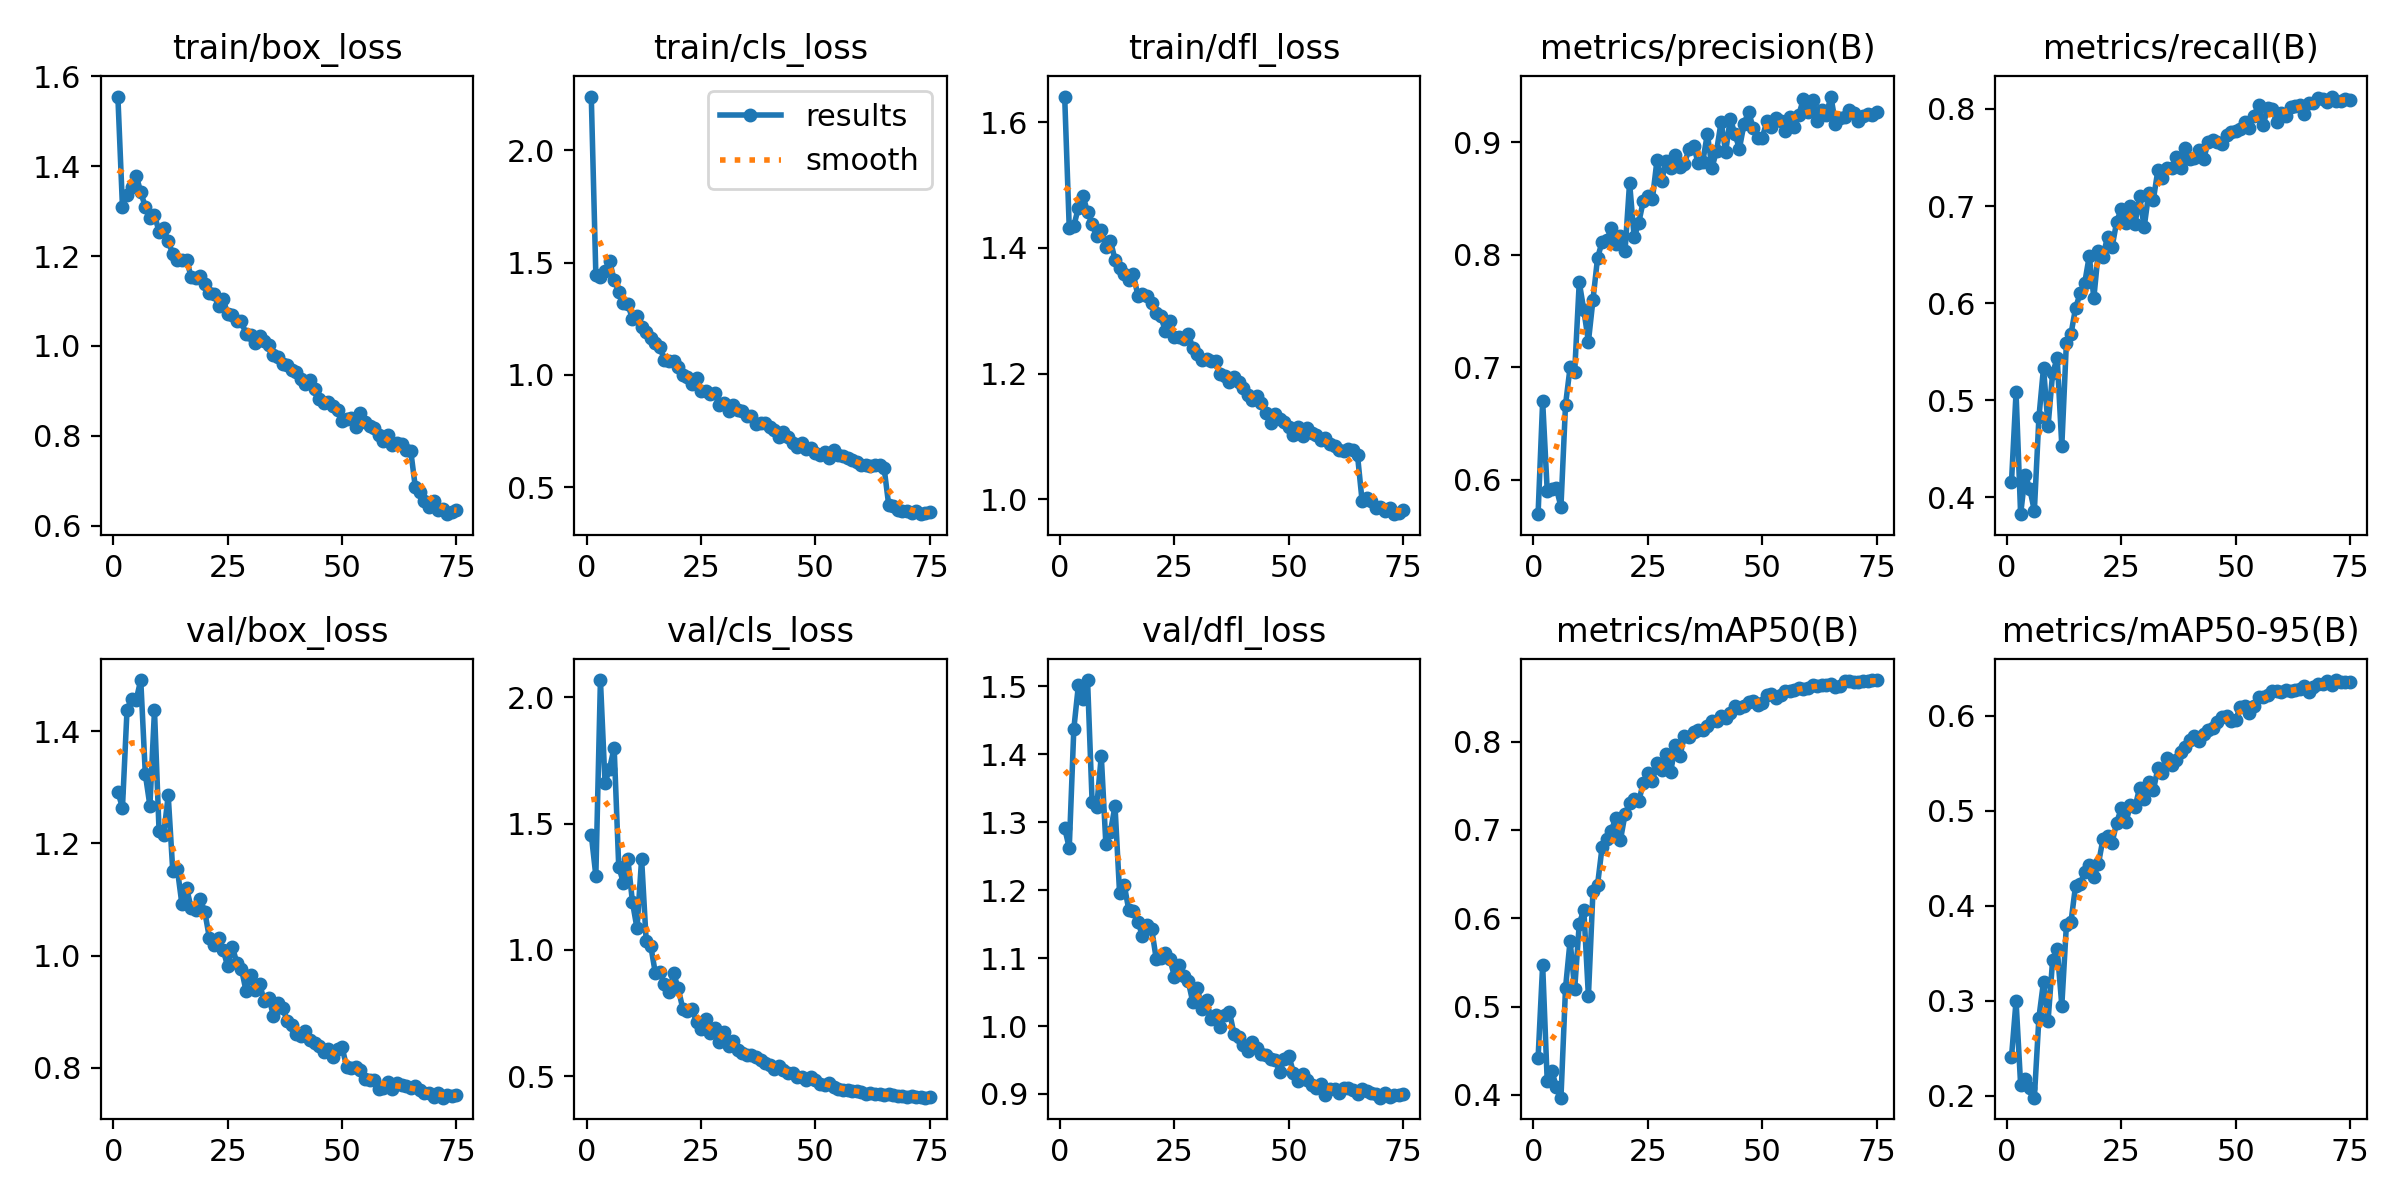
\includegraphics[width=\linewidth,height=0.4\textheight,keepaspectratio]{yolo11m_ppe_results.png}
\caption{Per-epoch losses and metrics as plotted by Ultralytics during training.}
\label{fig:runresults}
\end{figure}

\begin{figure}[htbp]
\centering
\begin{subfigure}{0.49\linewidth}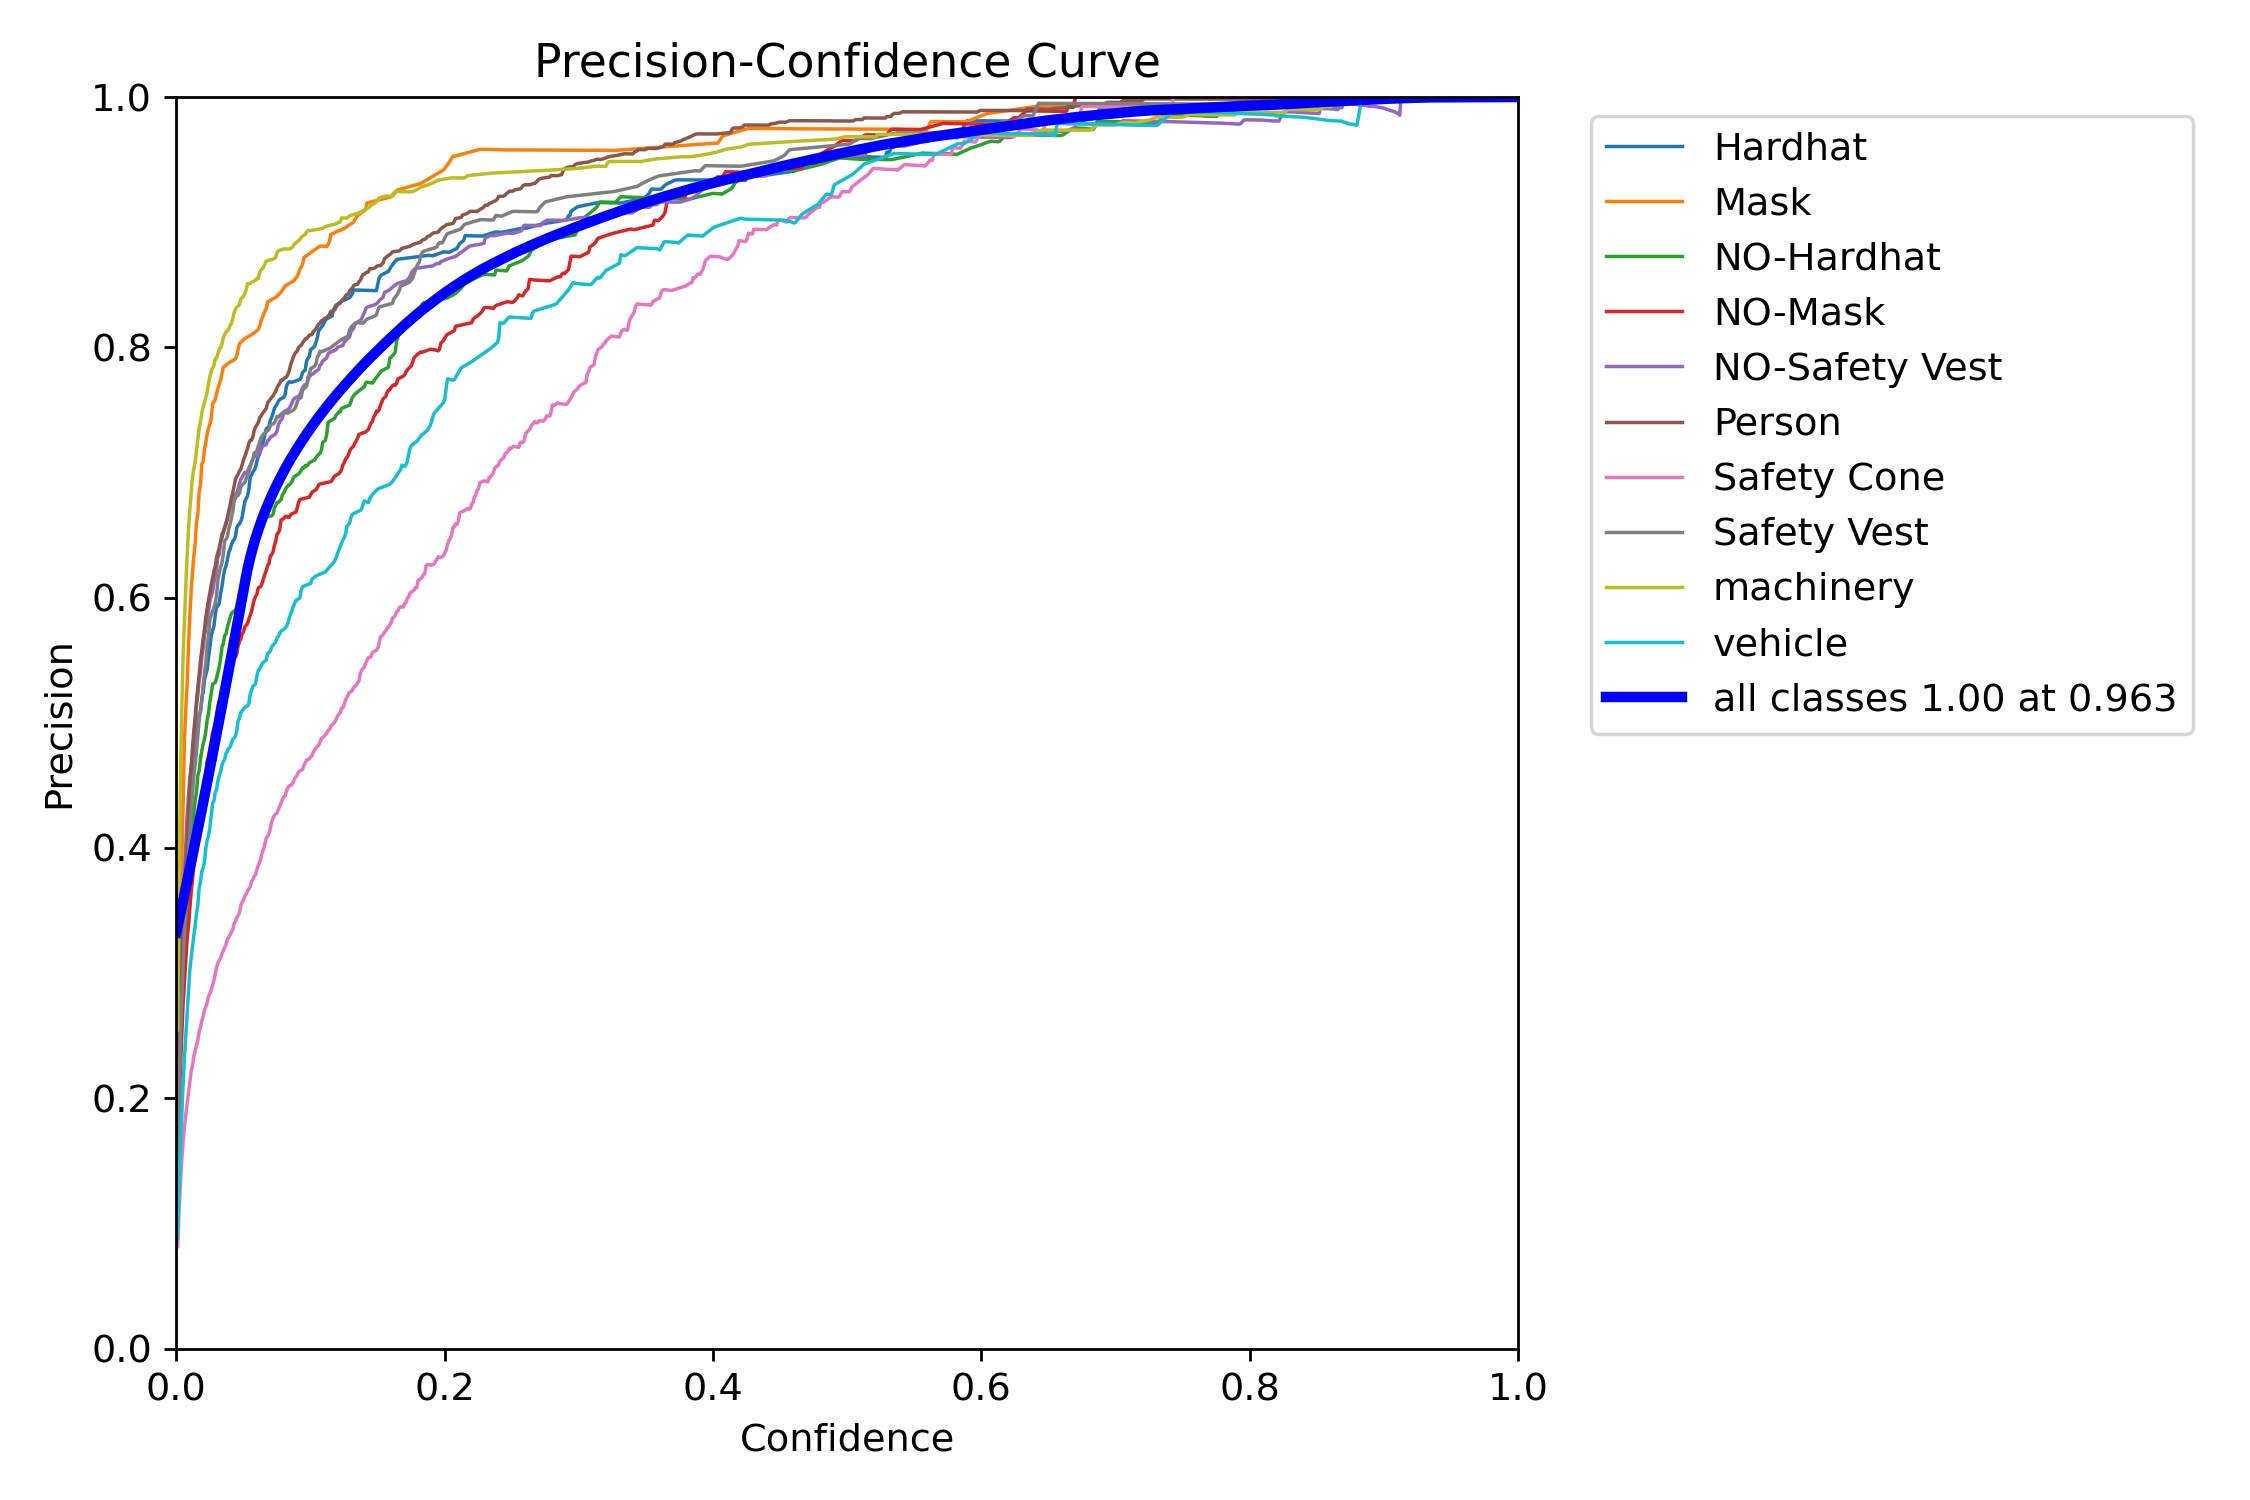
\includegraphics[width=\linewidth]{yolo11m_ppe_BoxP_curve.png}\caption{Precision}\end{subfigure}\hfill
\begin{subfigure}{0.49\linewidth}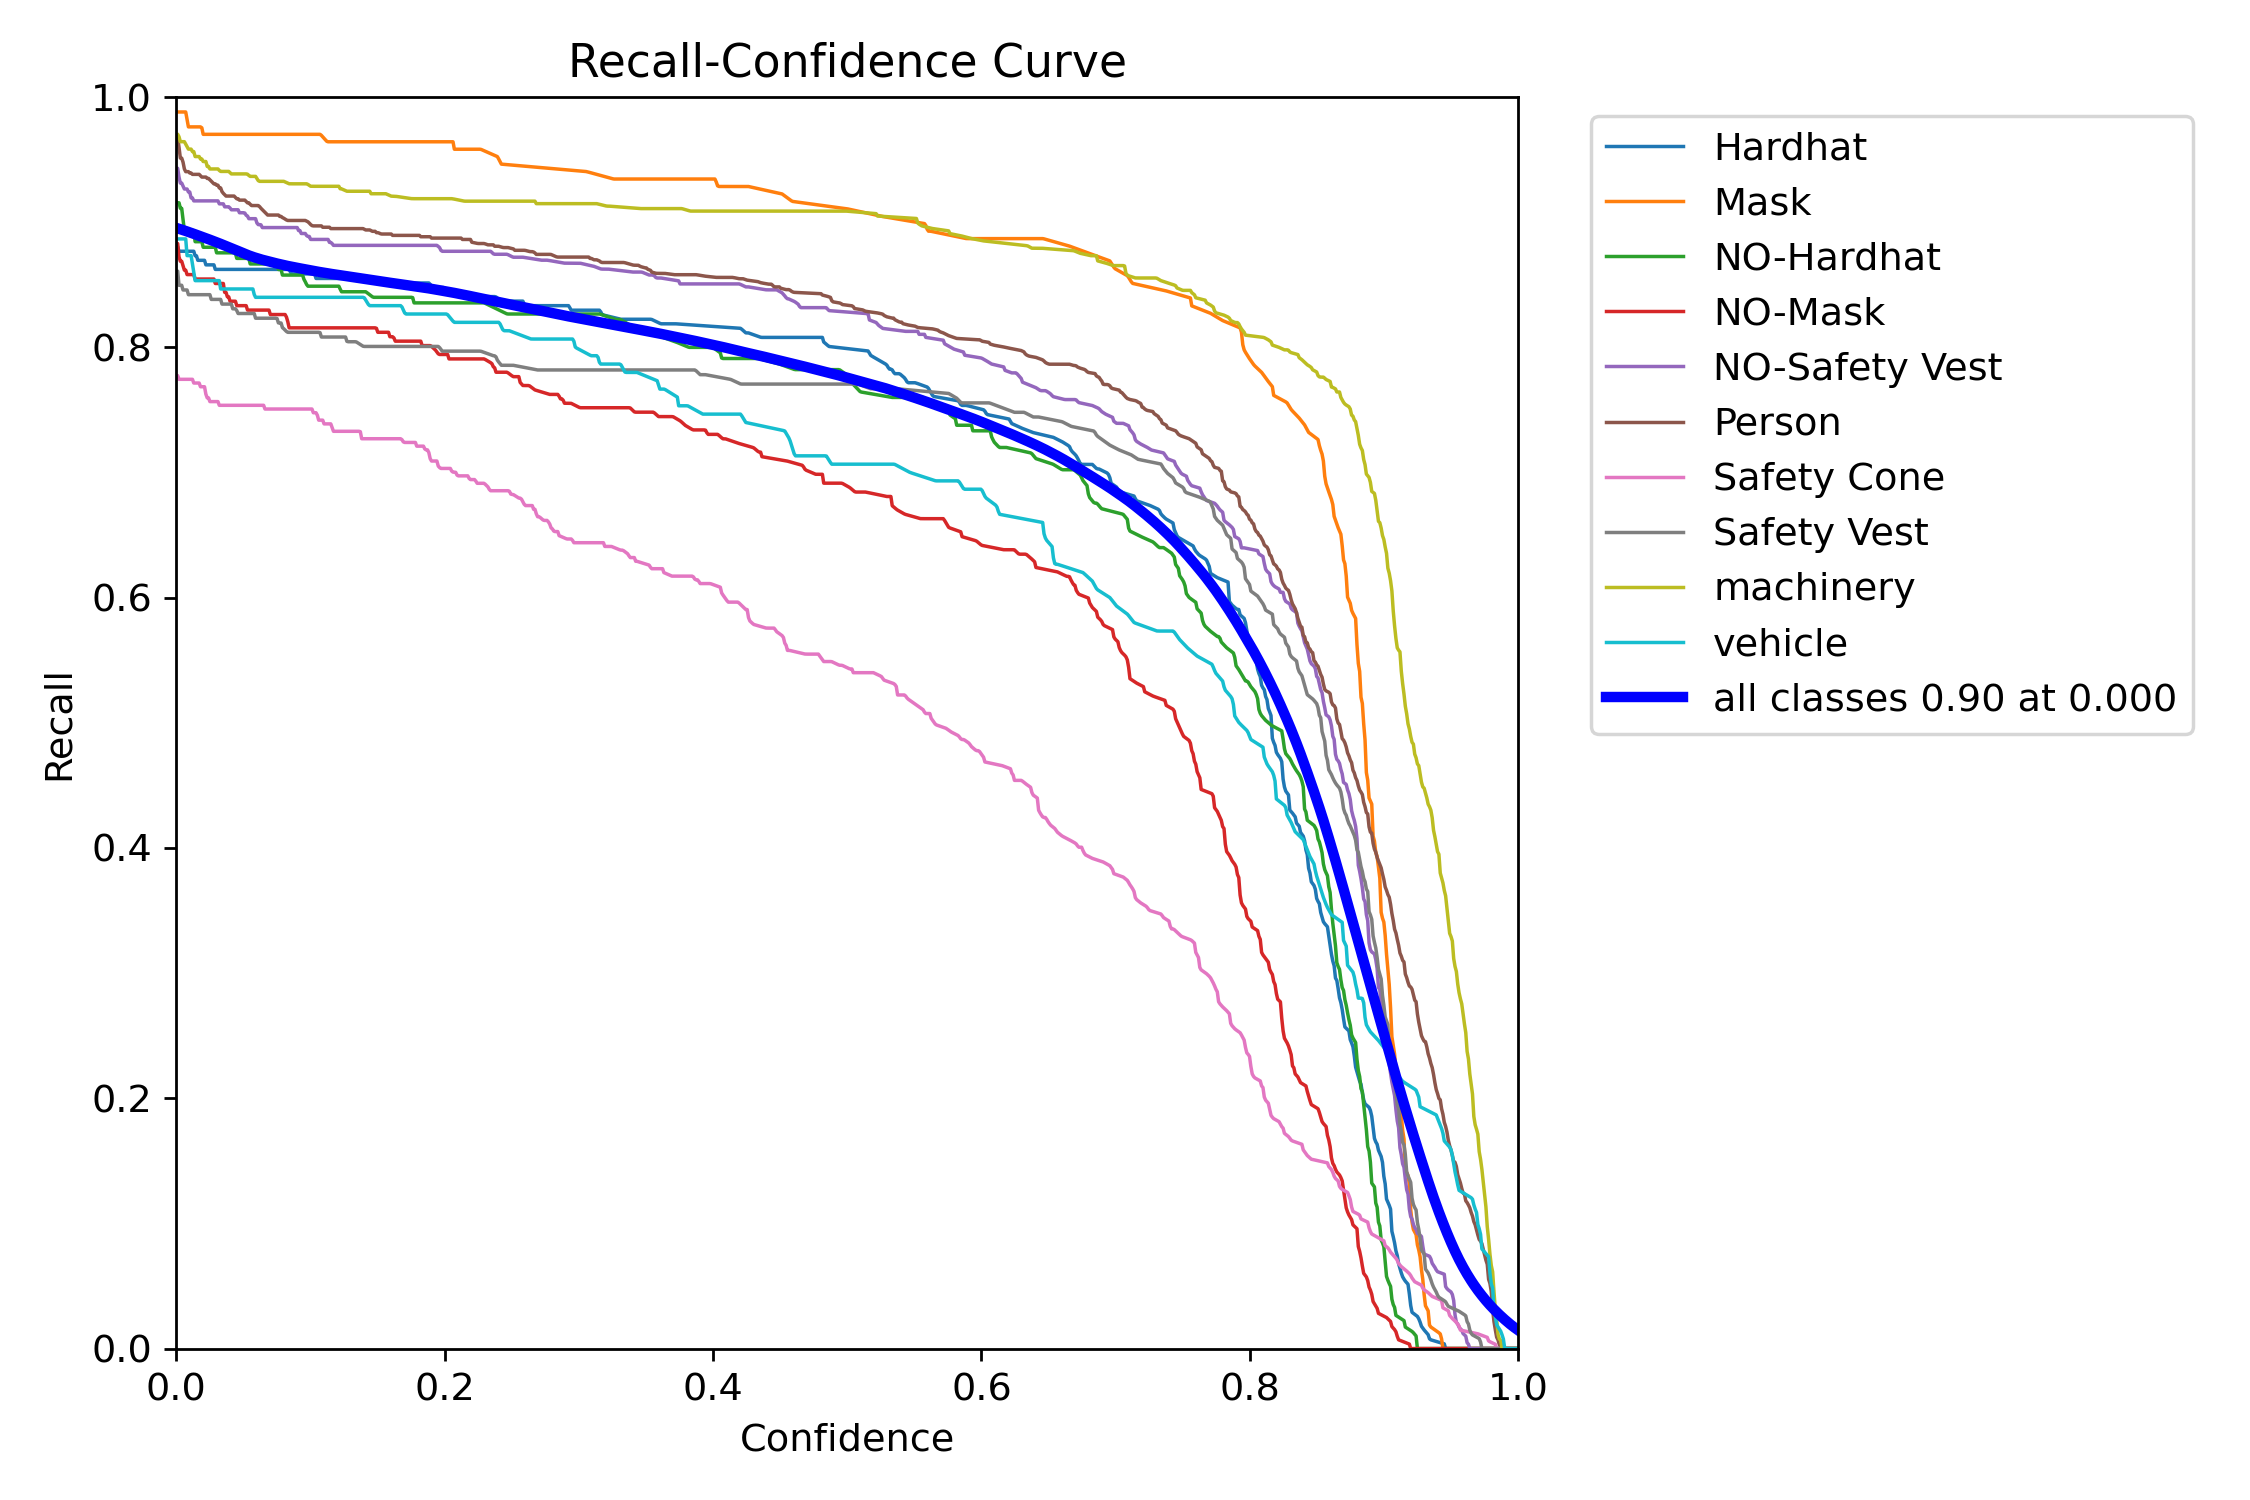
\includegraphics[width=\linewidth]{yolo11m_ppe_BoxR_curve.png}\caption{Recall}\end{subfigure}\\[2mm]
\begin{subfigure}{0.49\linewidth}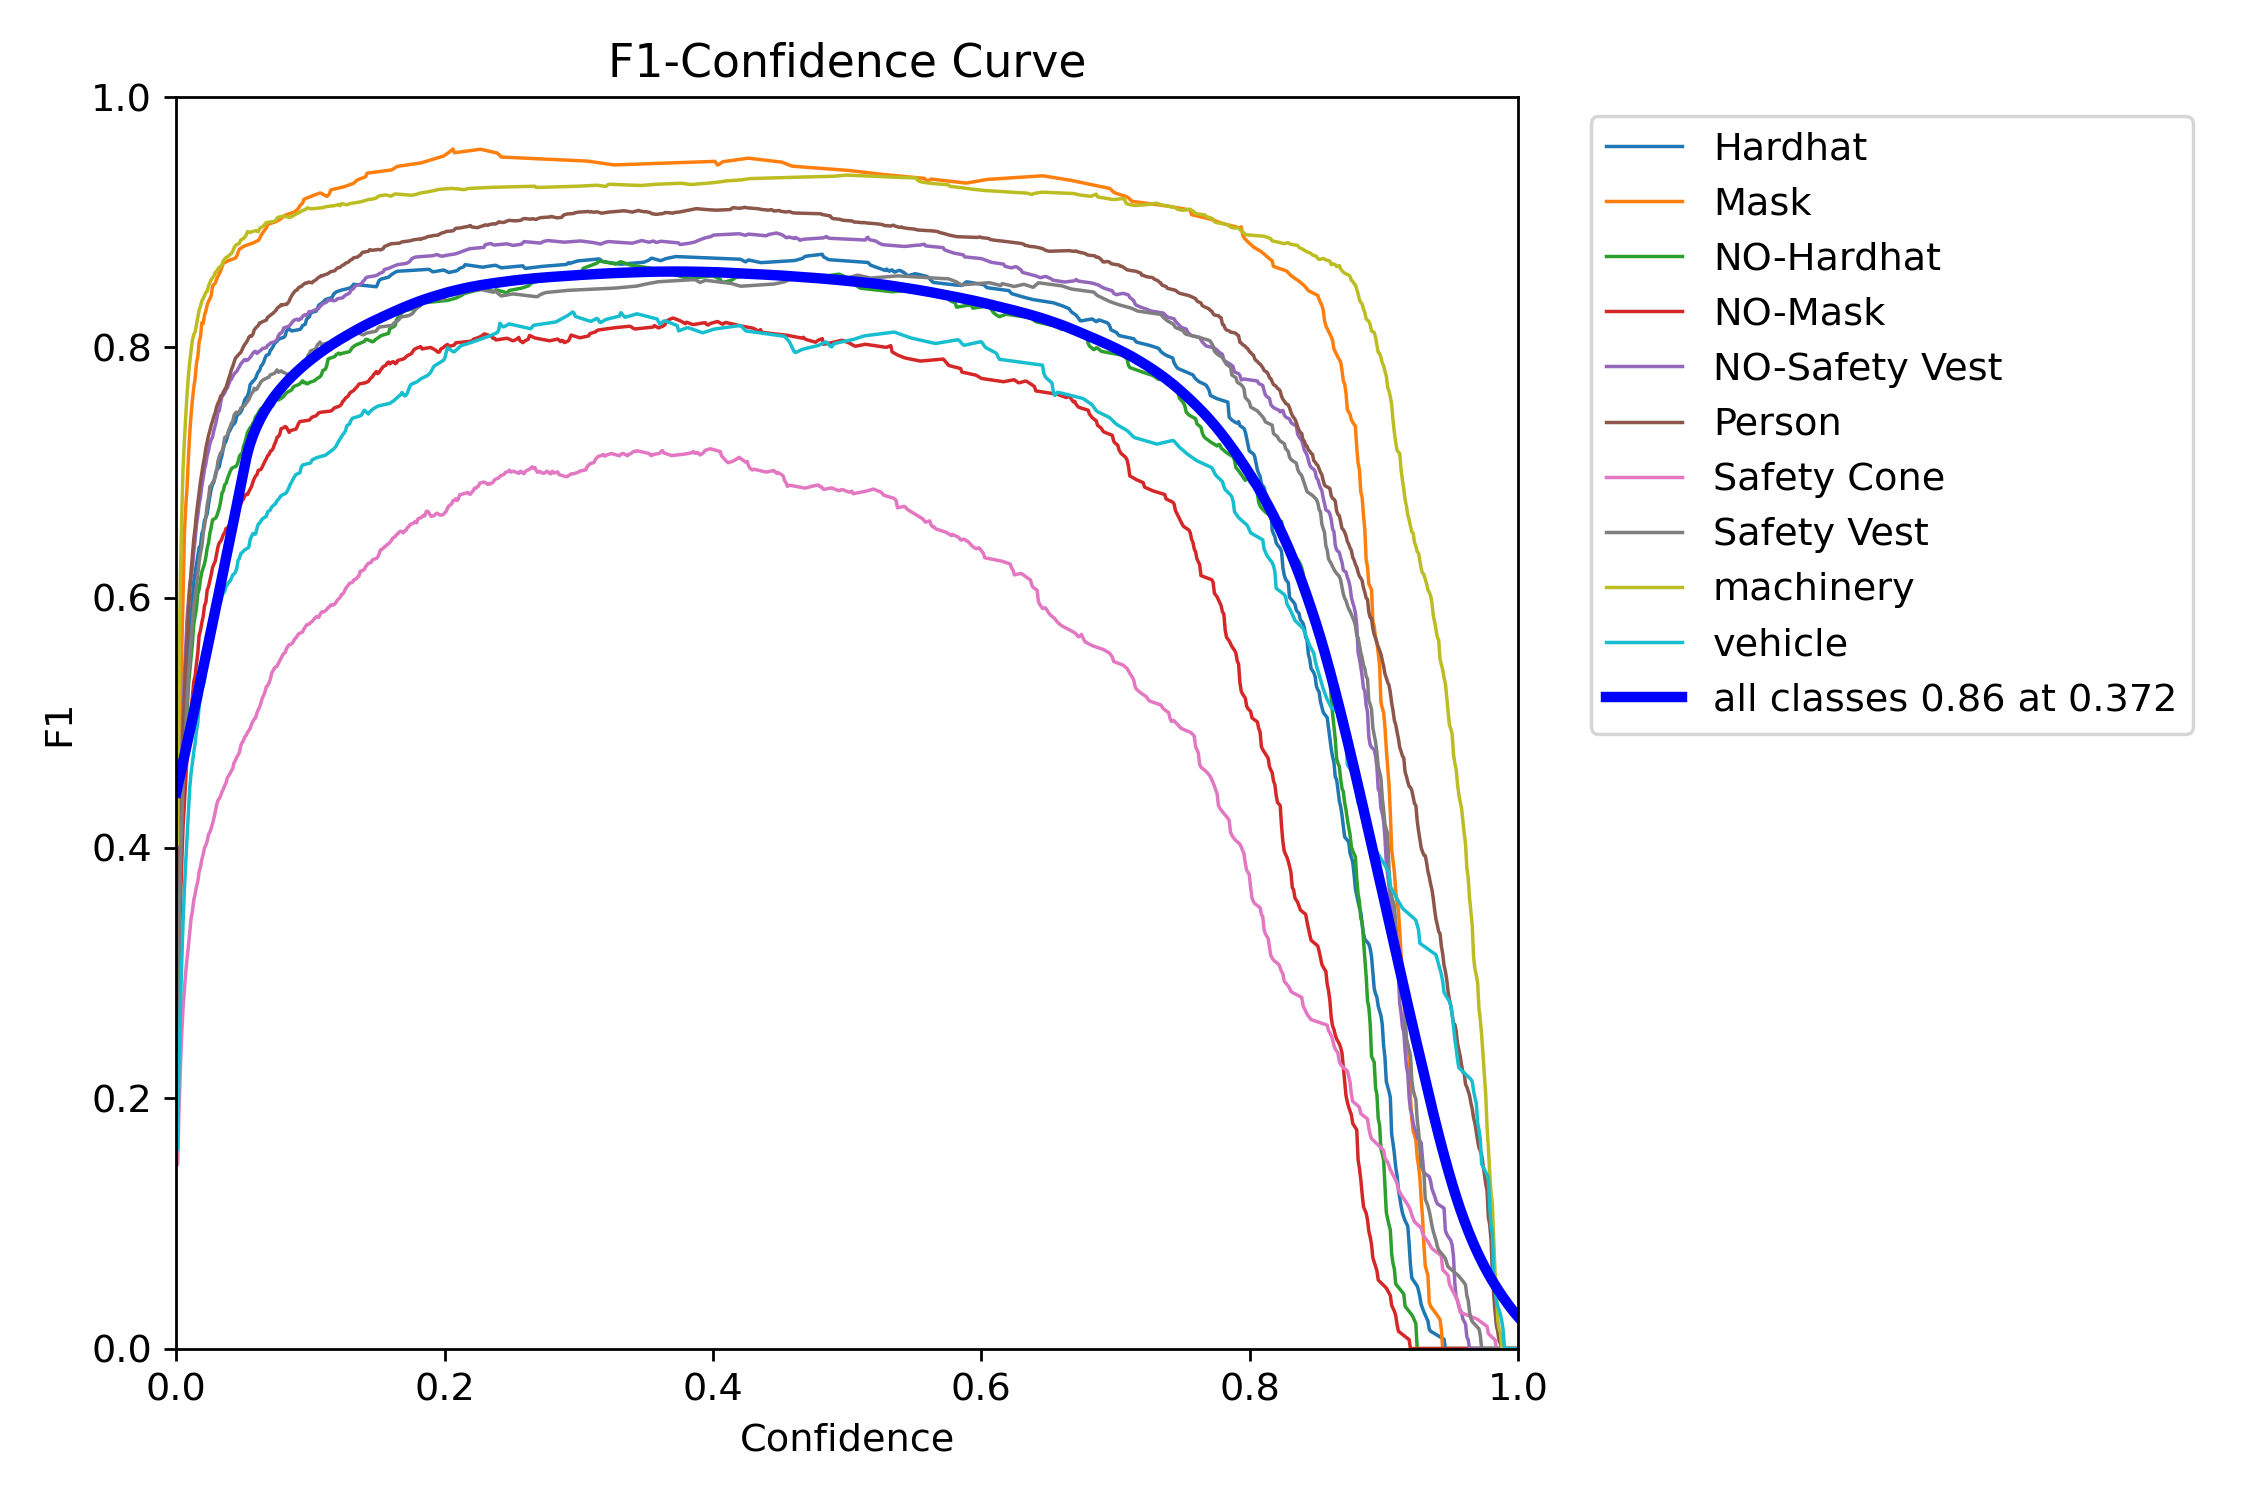
\includegraphics[width=\linewidth]{yolo11m_ppe_BoxF1_curve.png}\caption{F1}\end{subfigure}\hfill
\begin{subfigure}{0.49\linewidth}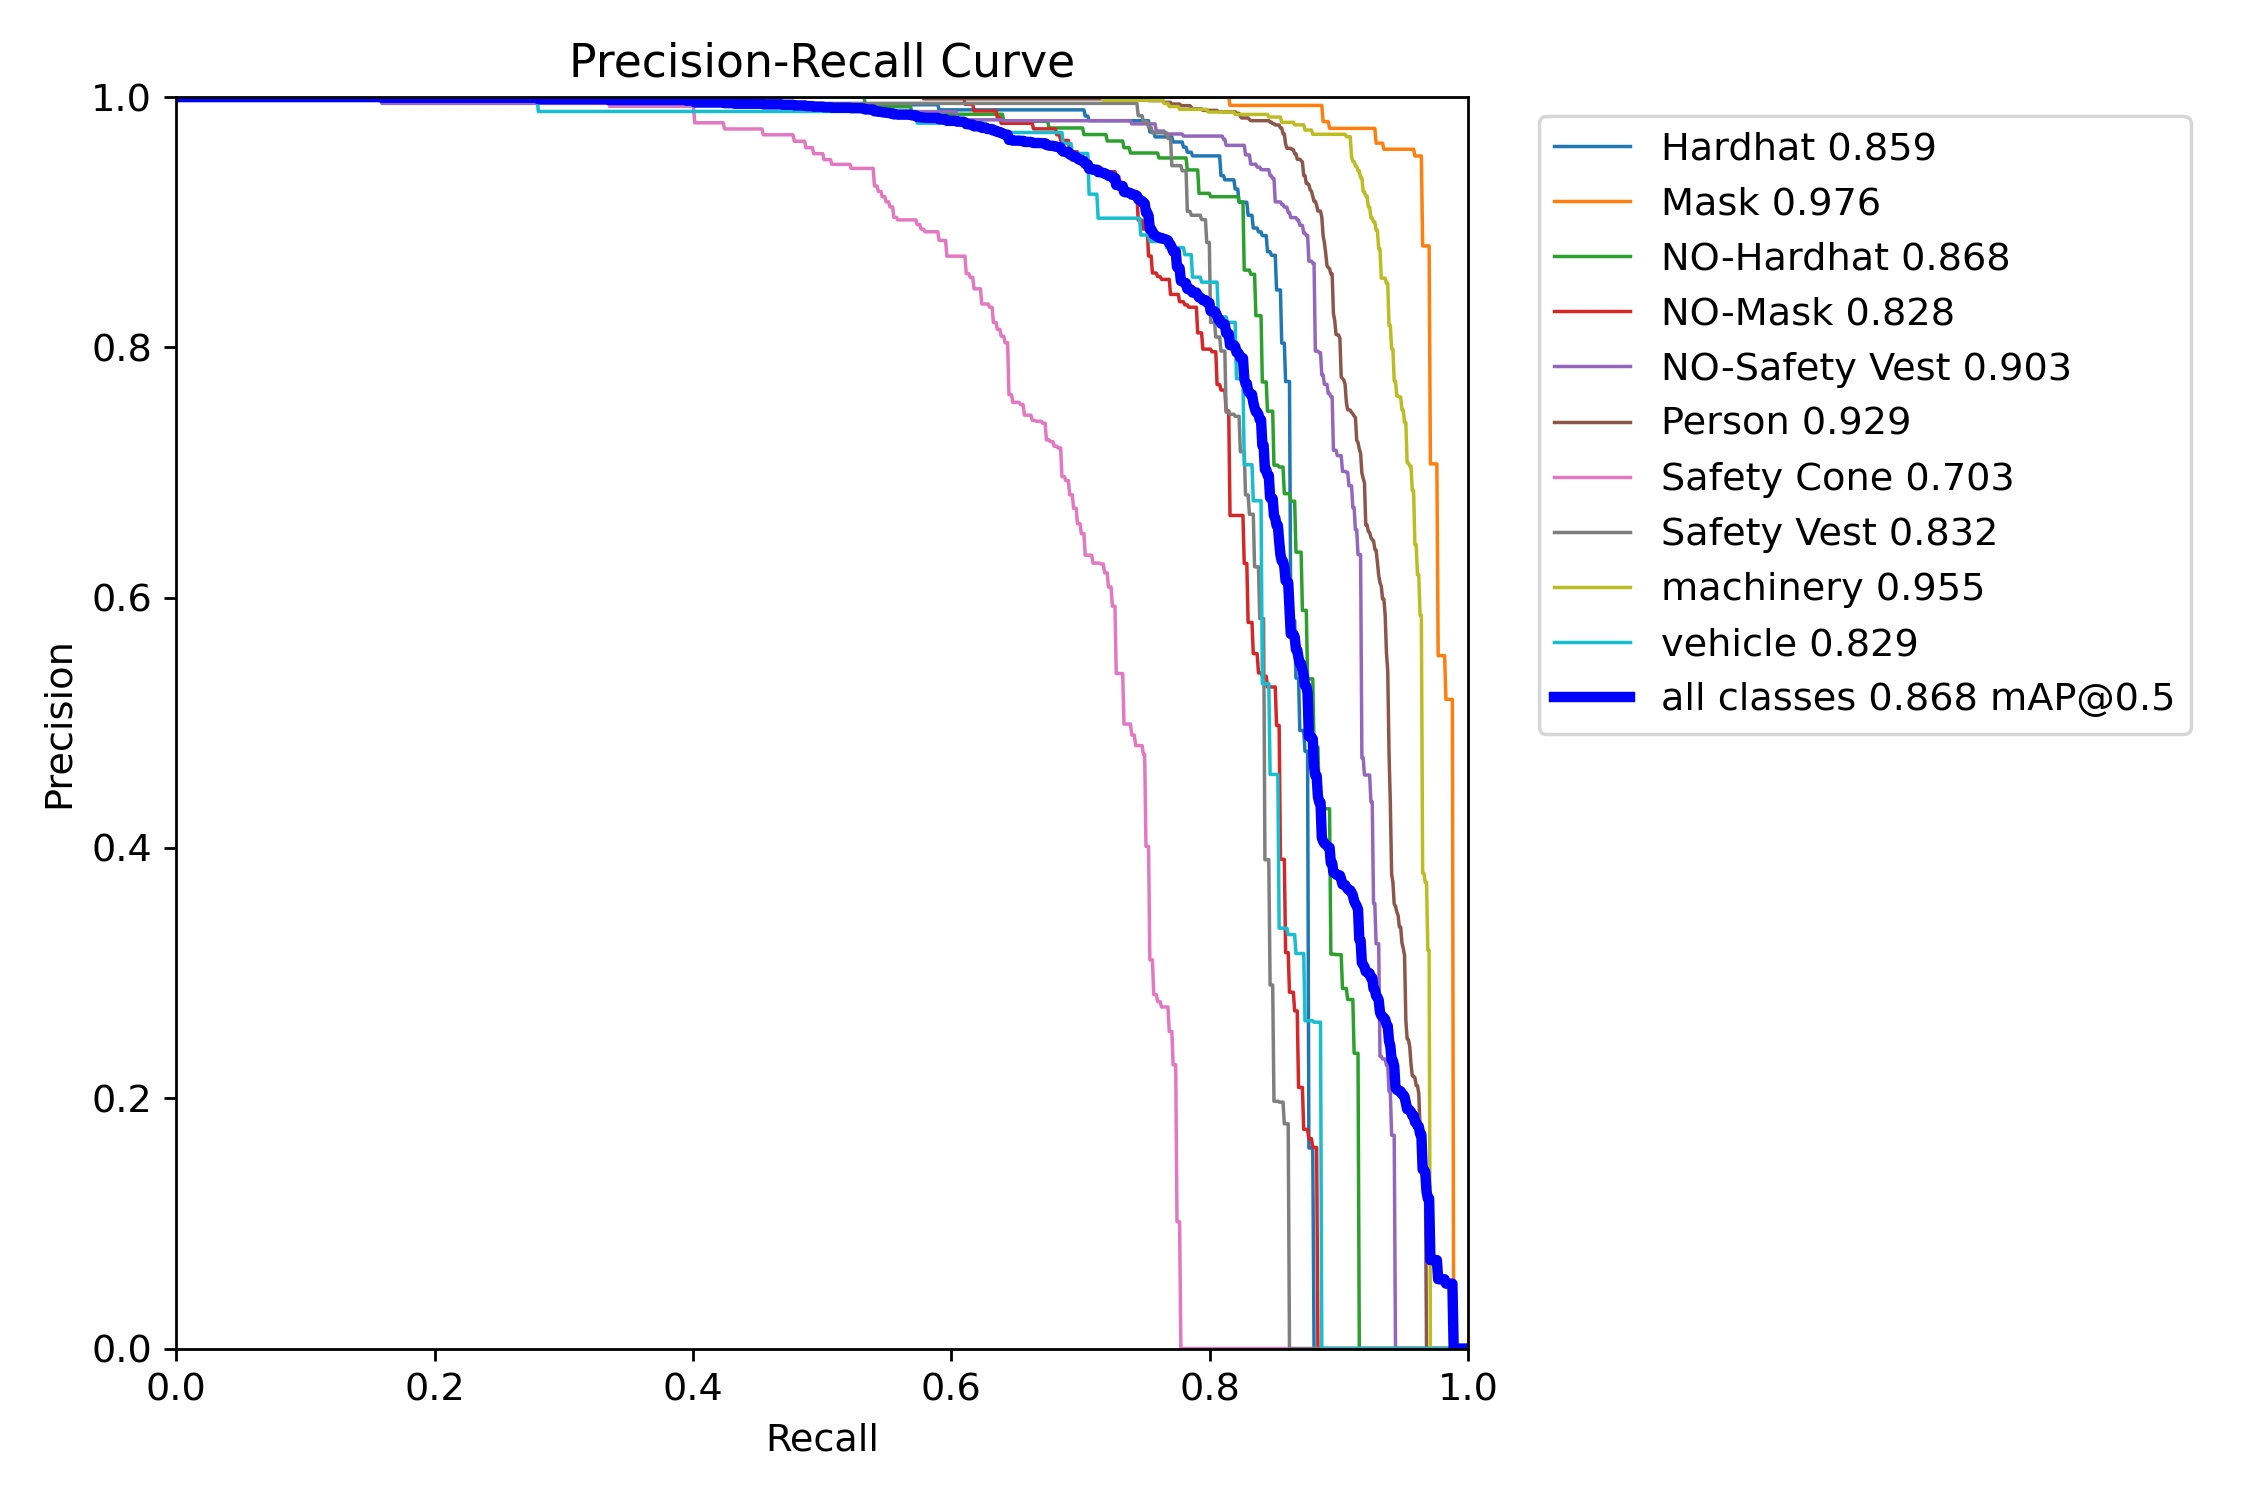
\includegraphics[width=\linewidth]{yolo11m_ppe_BoxPR_curve.png}\caption{Precision-recall}\end{subfigure}
\caption{Curves from the end-of-training validation of \texttt{best.pt}.}
\label{fig:runcurves}
\end{figure}

\begin{figure}[htbp]
\centering
\begin{subfigure}{0.49\linewidth}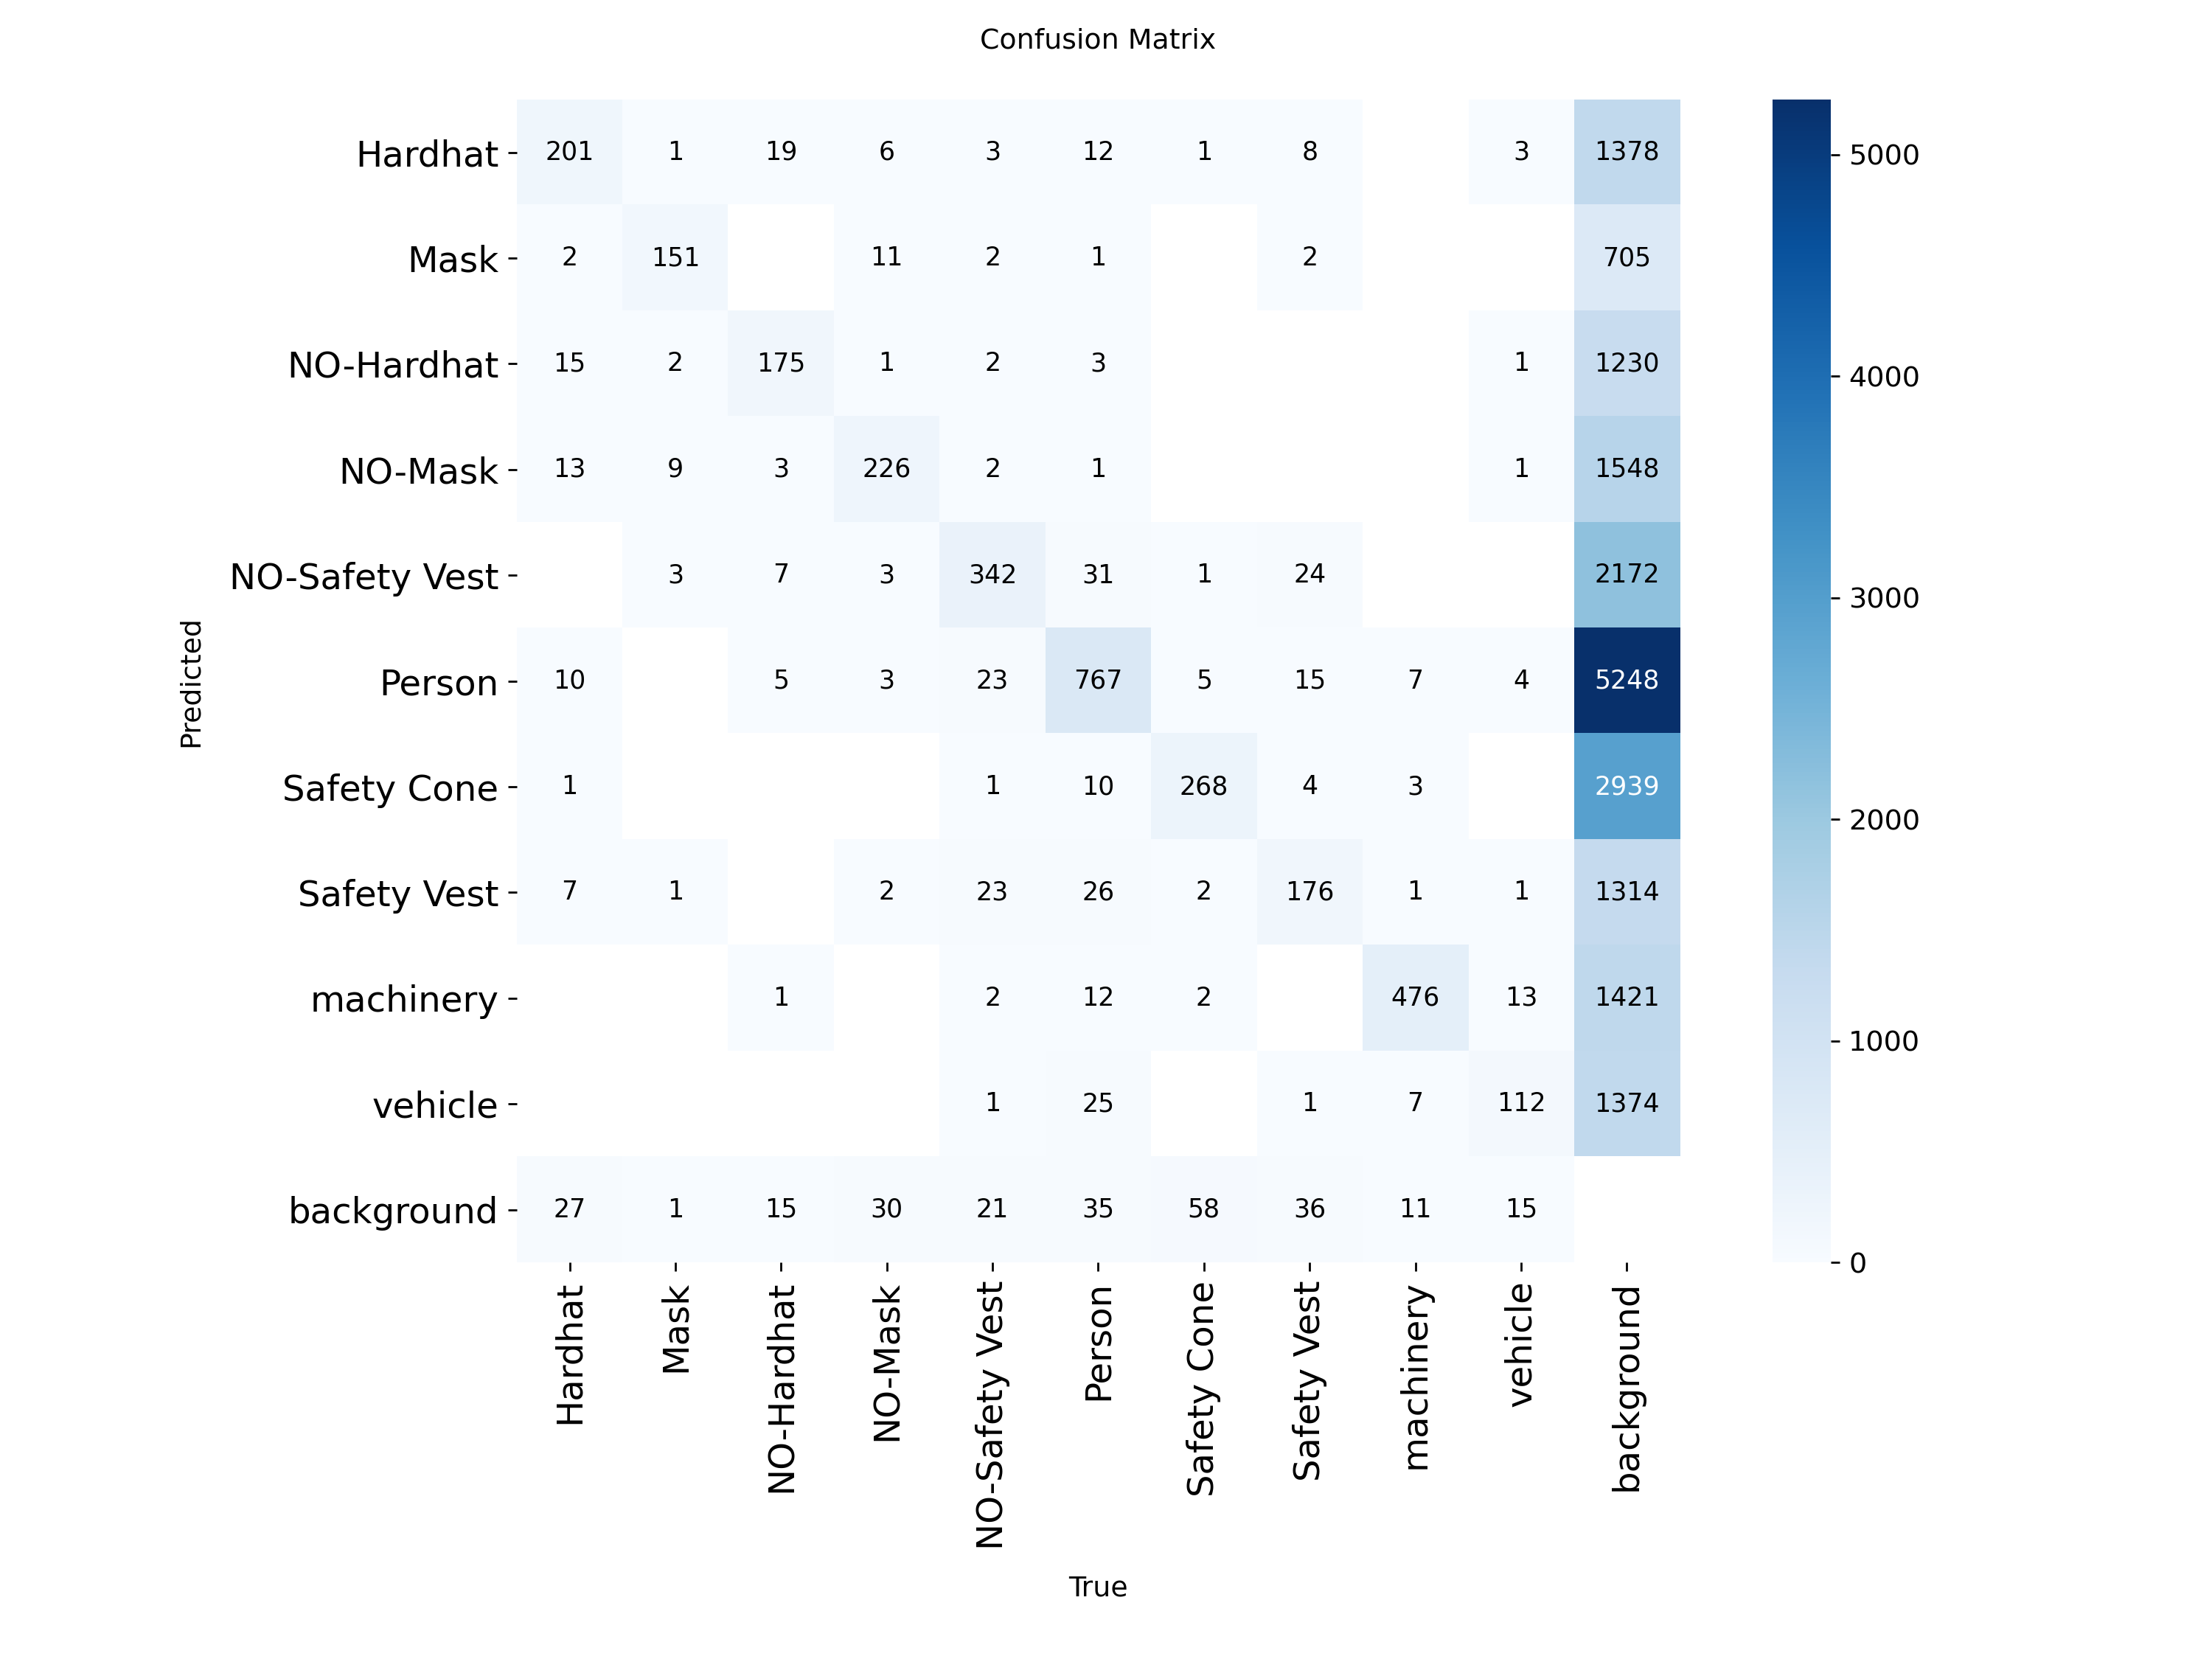
\includegraphics[width=\linewidth]{yolo11m_ppe_confusion_matrix.png}\caption{Counts}\end{subfigure}\hfill
\begin{subfigure}{0.49\linewidth}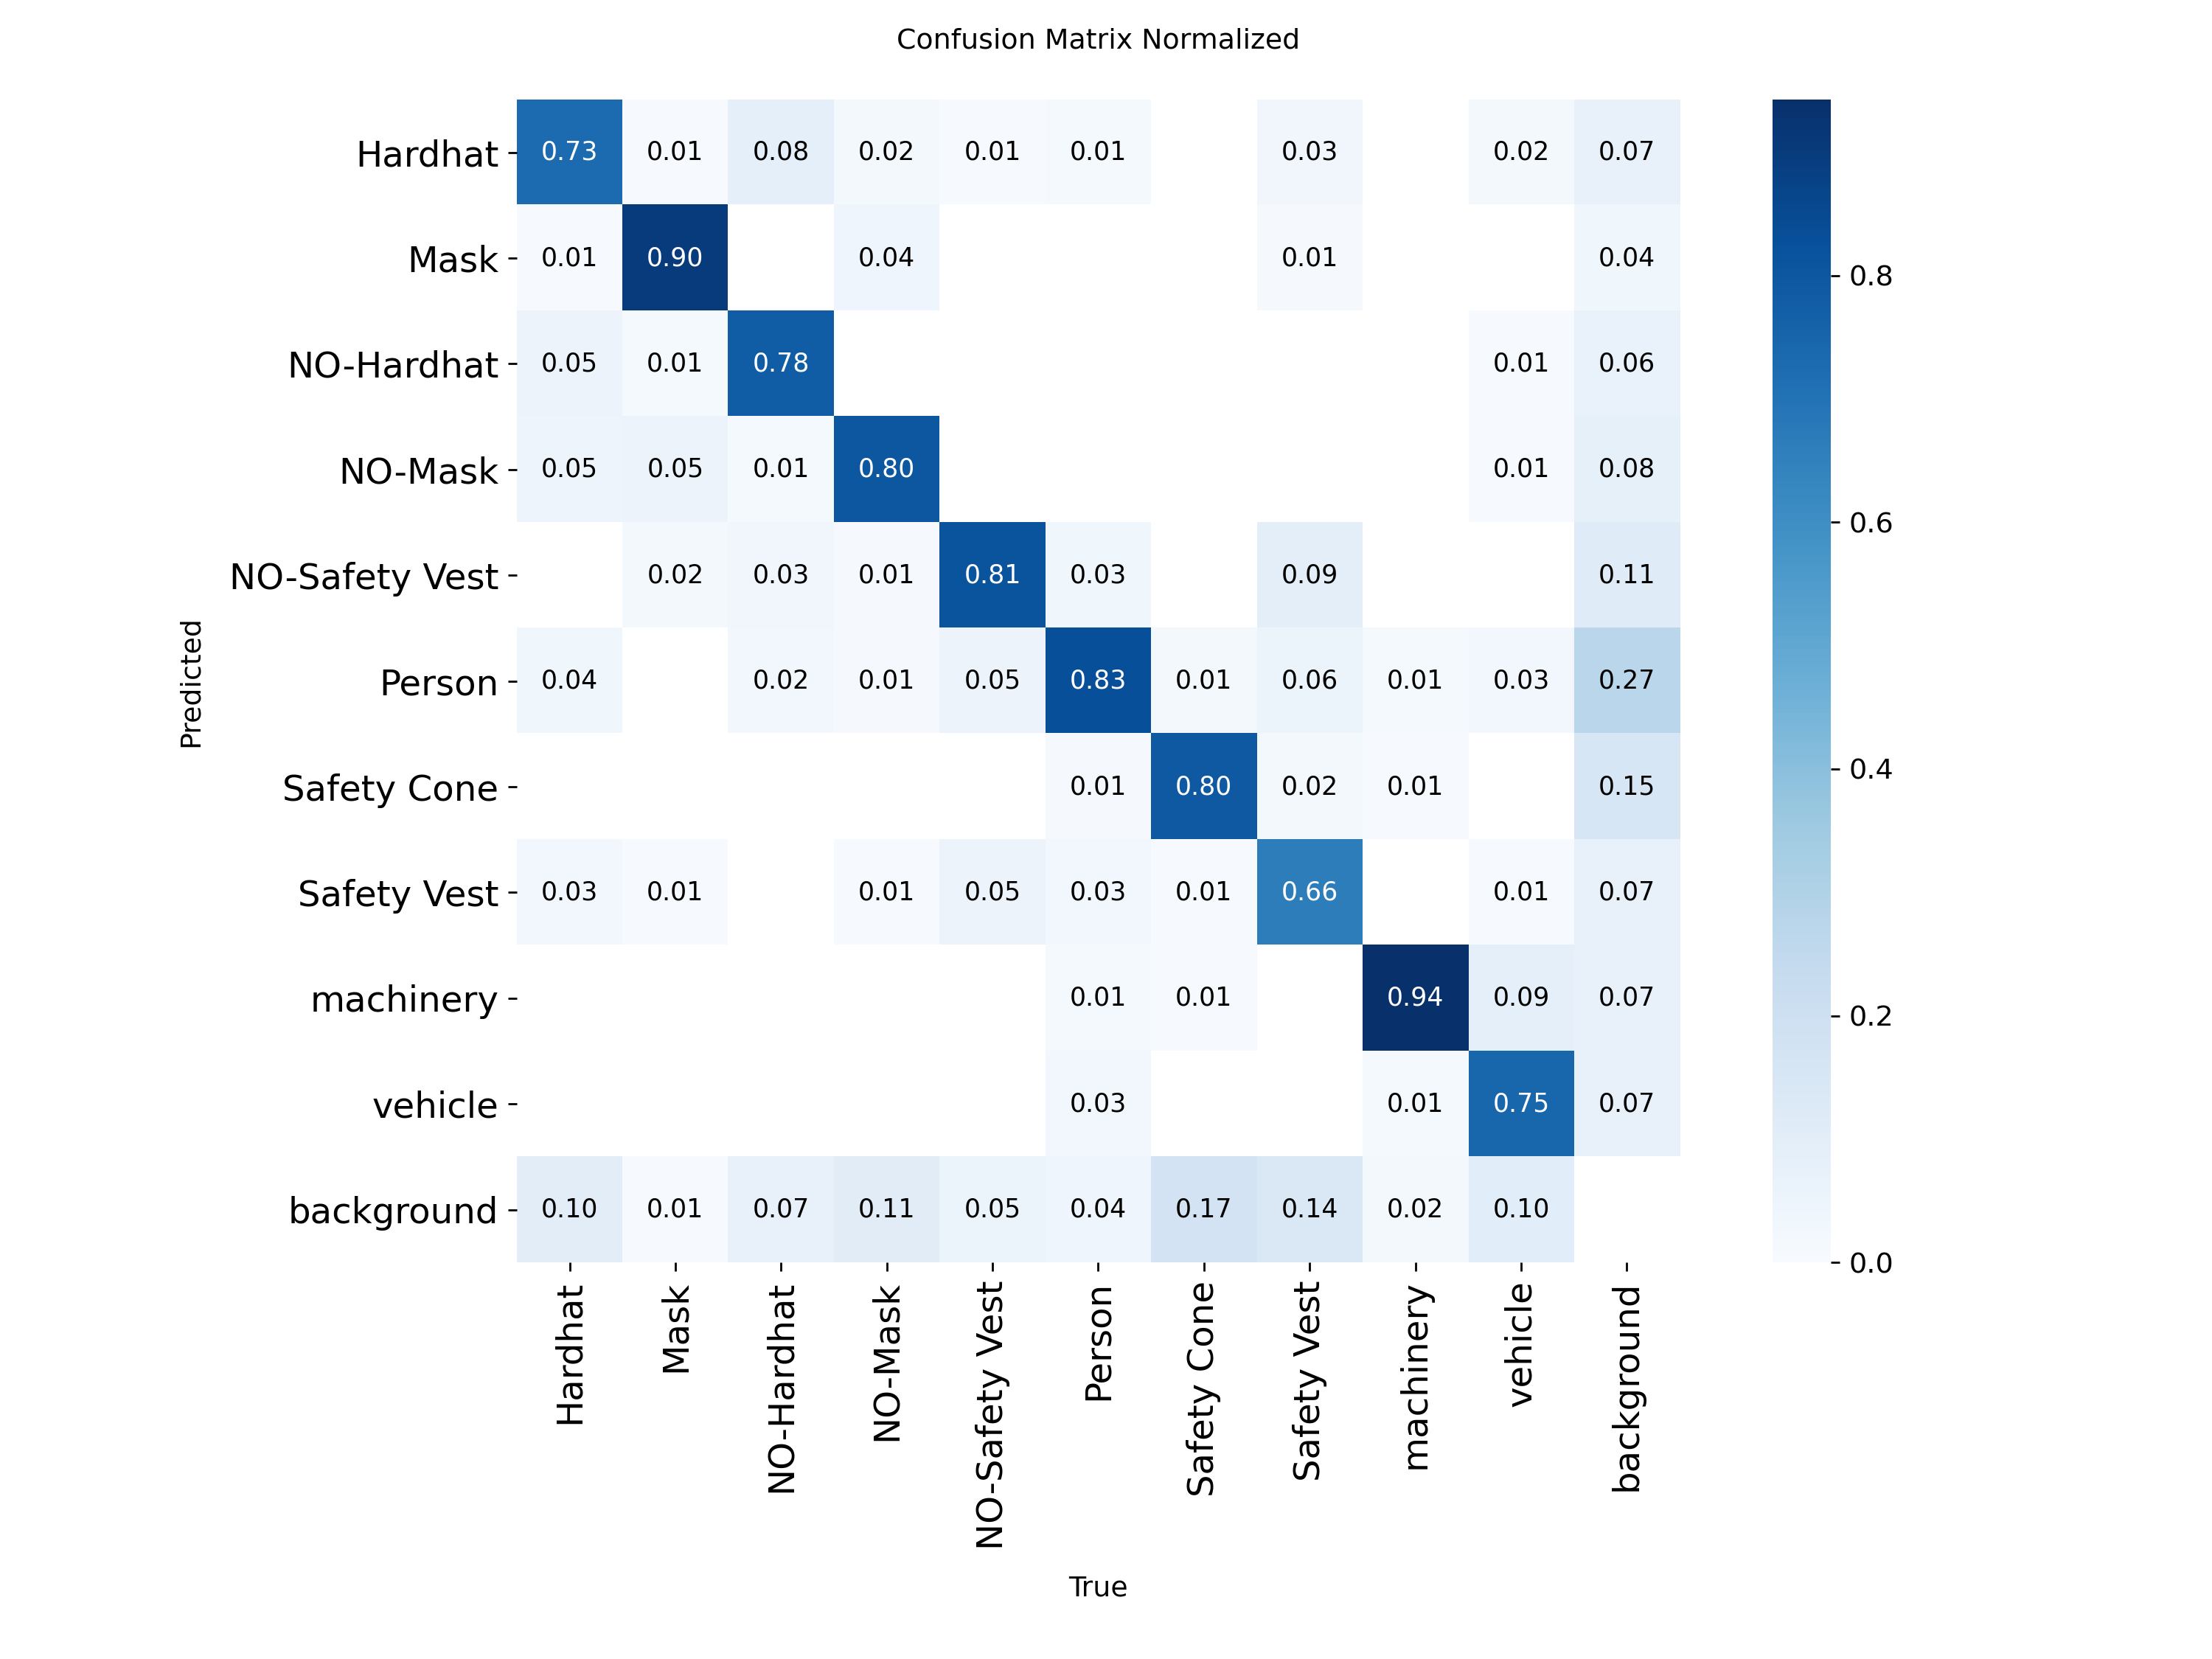
\includegraphics[width=\linewidth]{yolo11m_ppe_confusion_matrix_normalized.png}\caption{Normalised by true class}\end{subfigure}
\caption{Confusion matrices from the end-of-training validation of \texttt{best.pt}.}
\label{fig:runcm}
\end{figure}

\begin{figure}[htbp]
\centering
\begin{subfigure}{0.49\linewidth}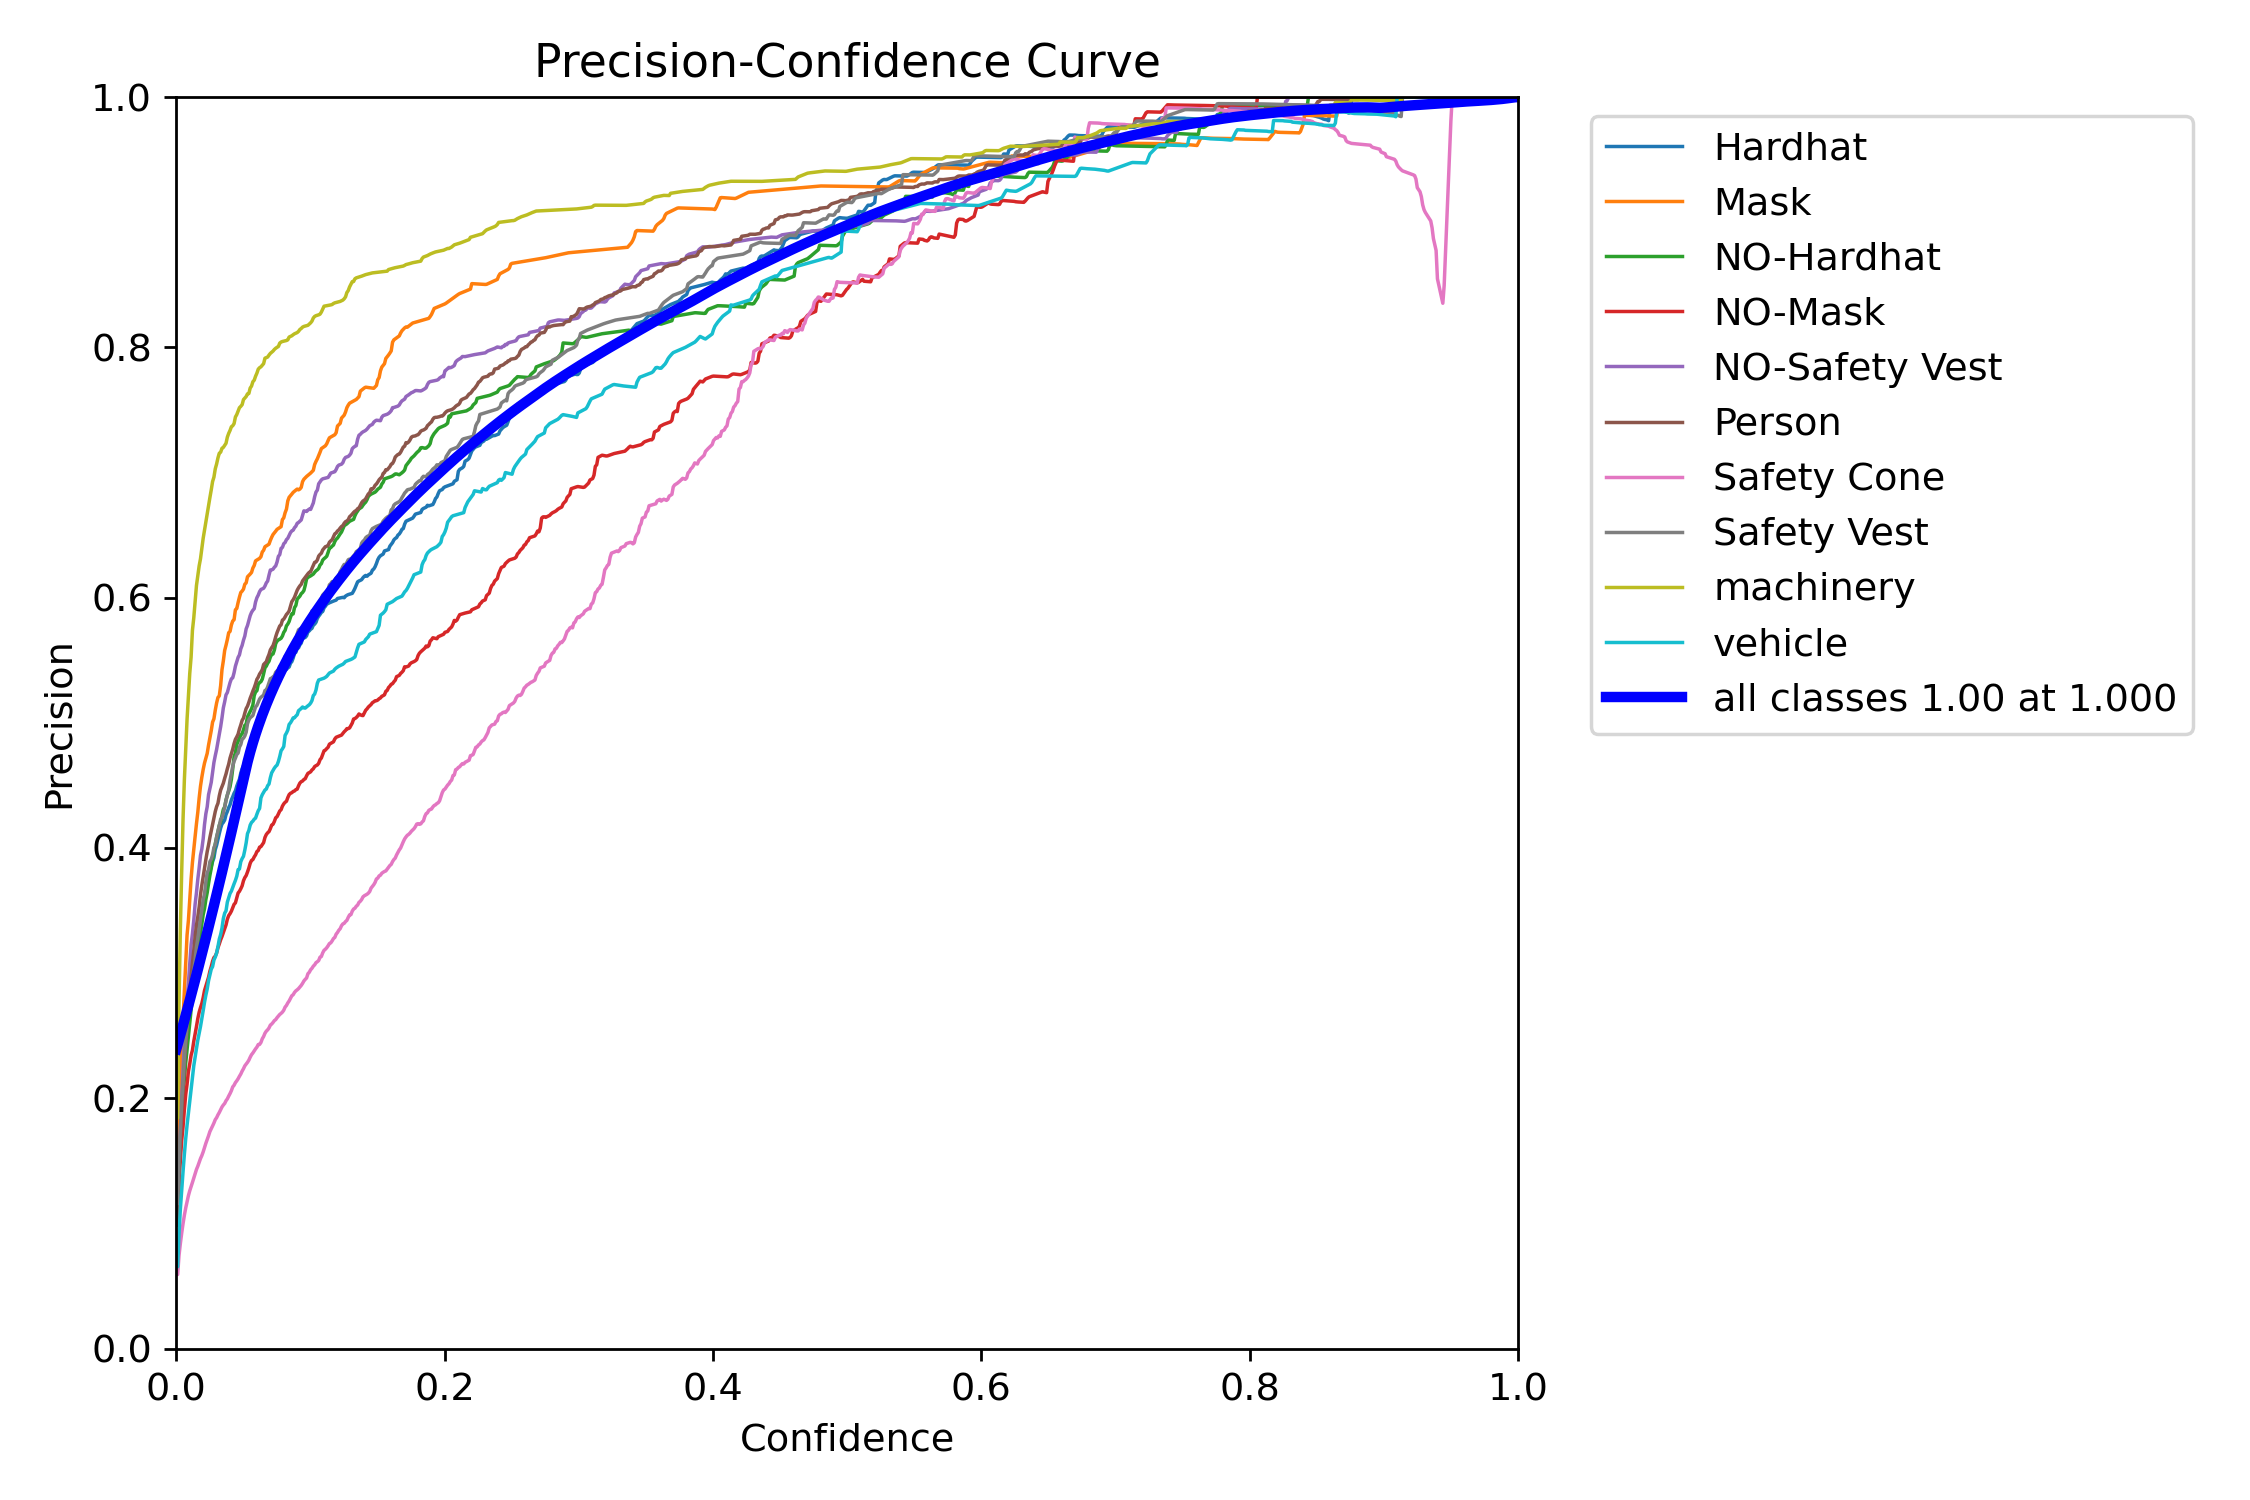
\includegraphics[width=\linewidth]{eval_test_tta_BoxP_curve.png}\caption{Precision}\end{subfigure}\hfill
\begin{subfigure}{0.49\linewidth}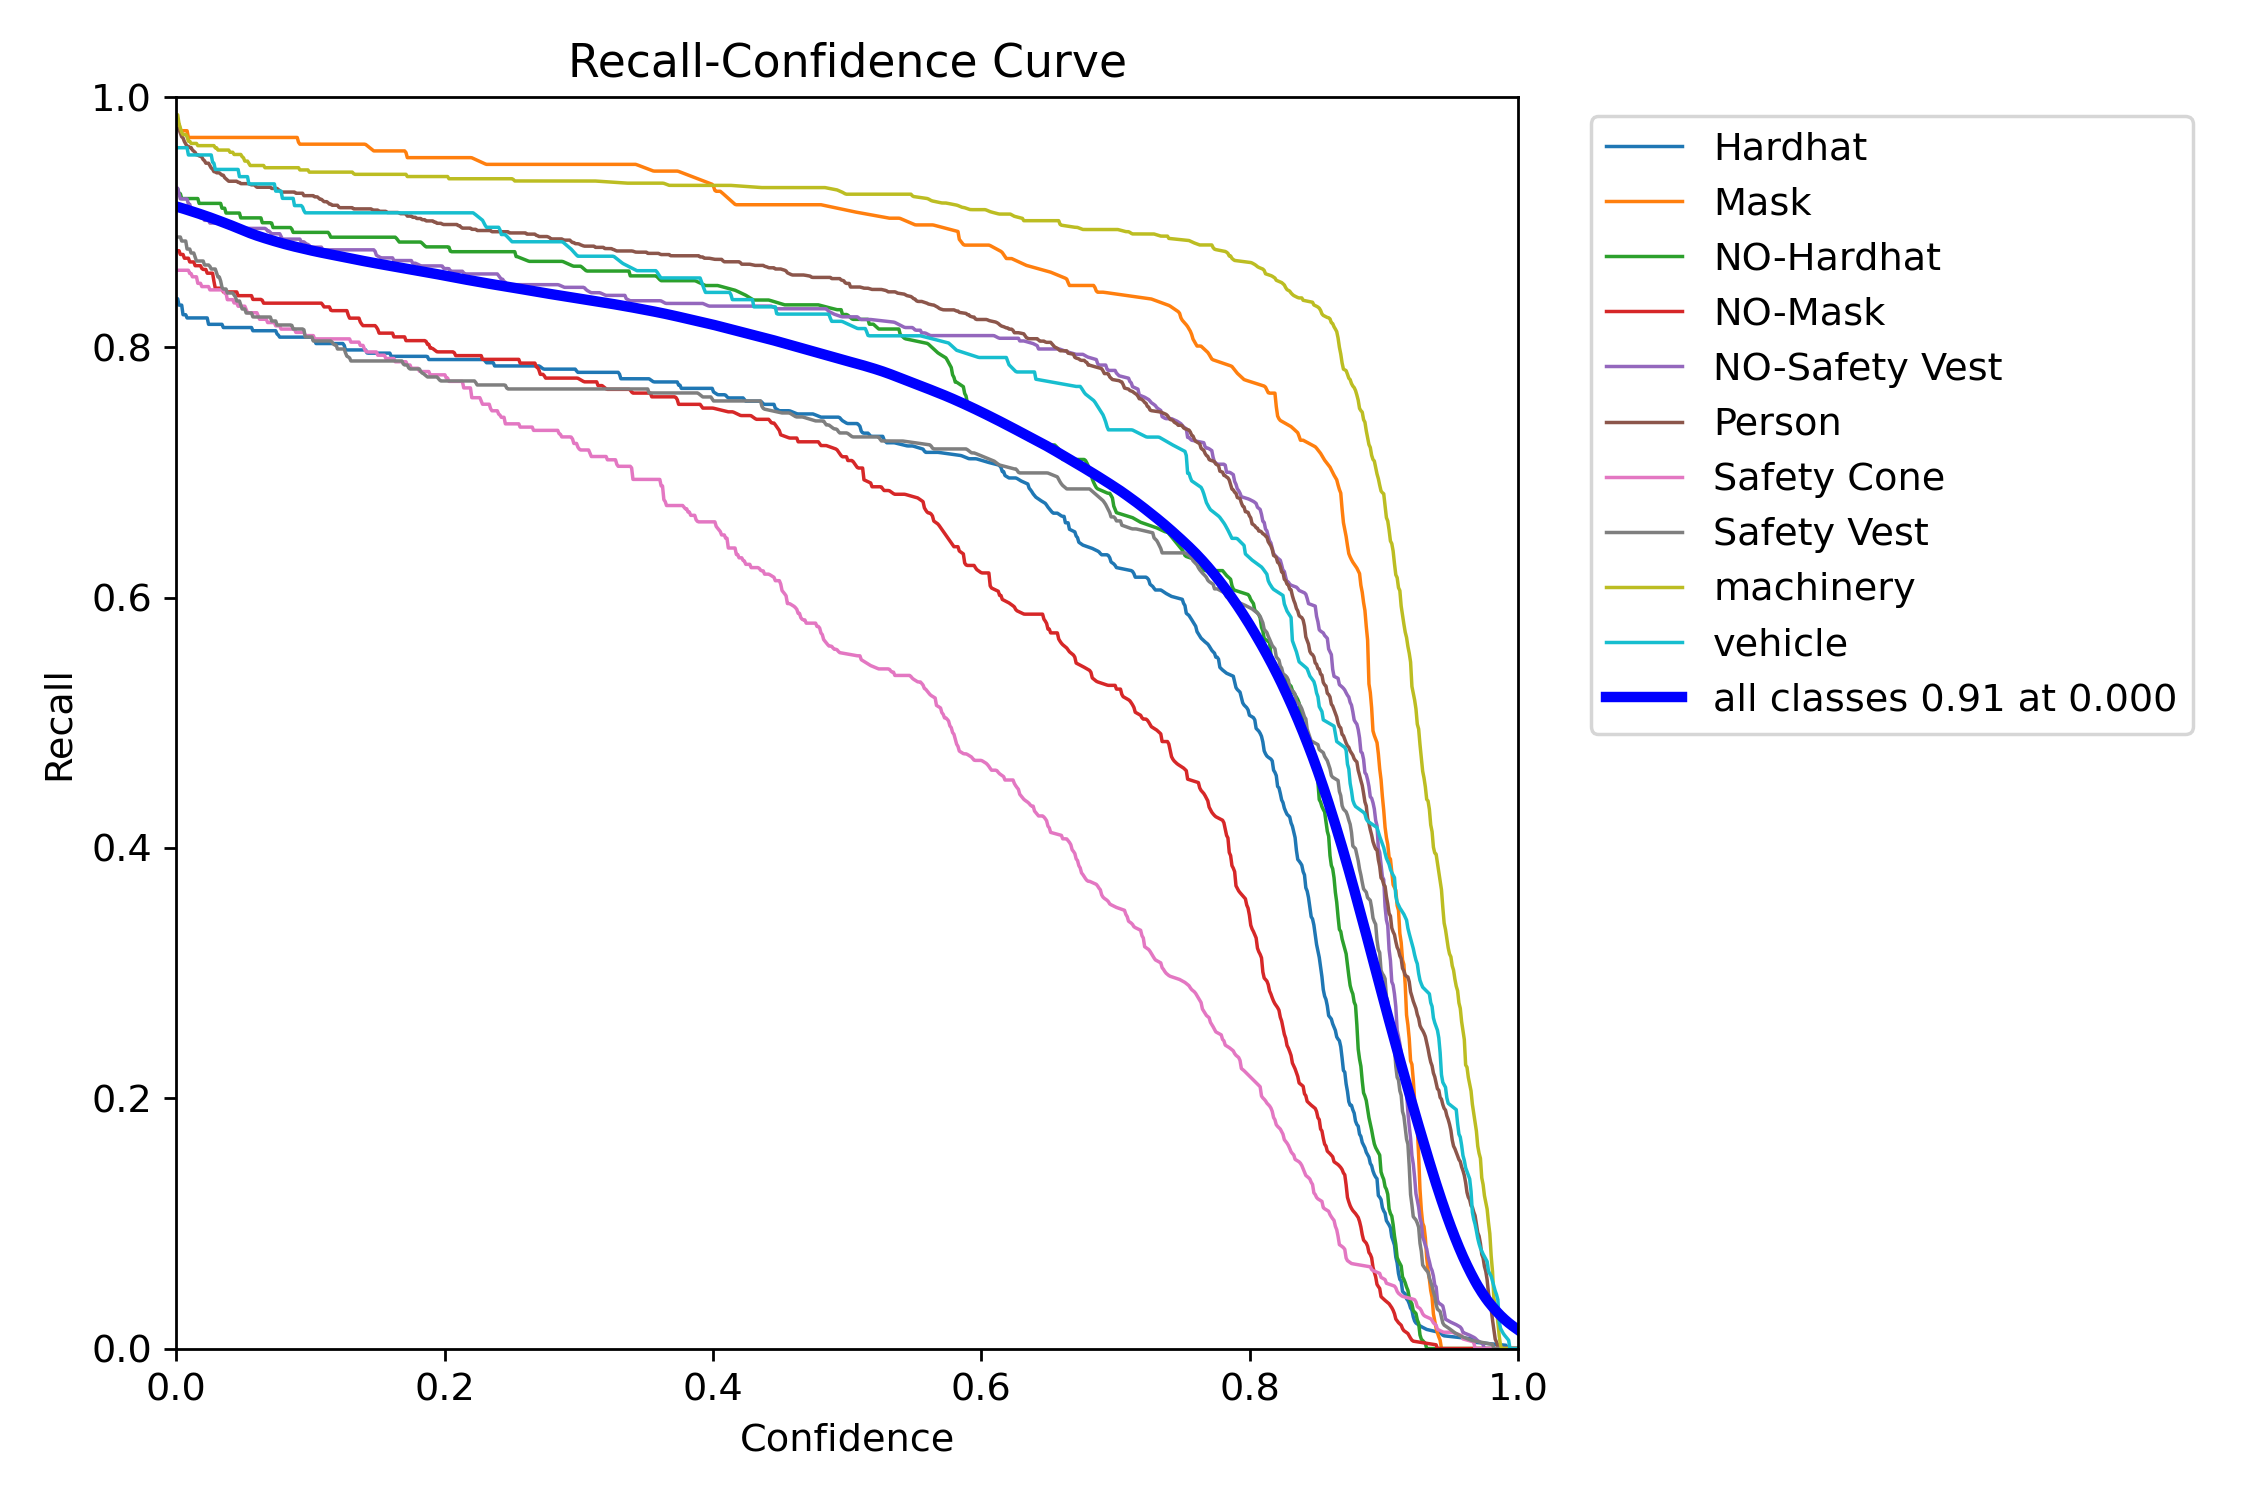
\includegraphics[width=\linewidth]{eval_test_tta_BoxR_curve.png}\caption{Recall}\end{subfigure}\\[2mm]
\begin{subfigure}{0.49\linewidth}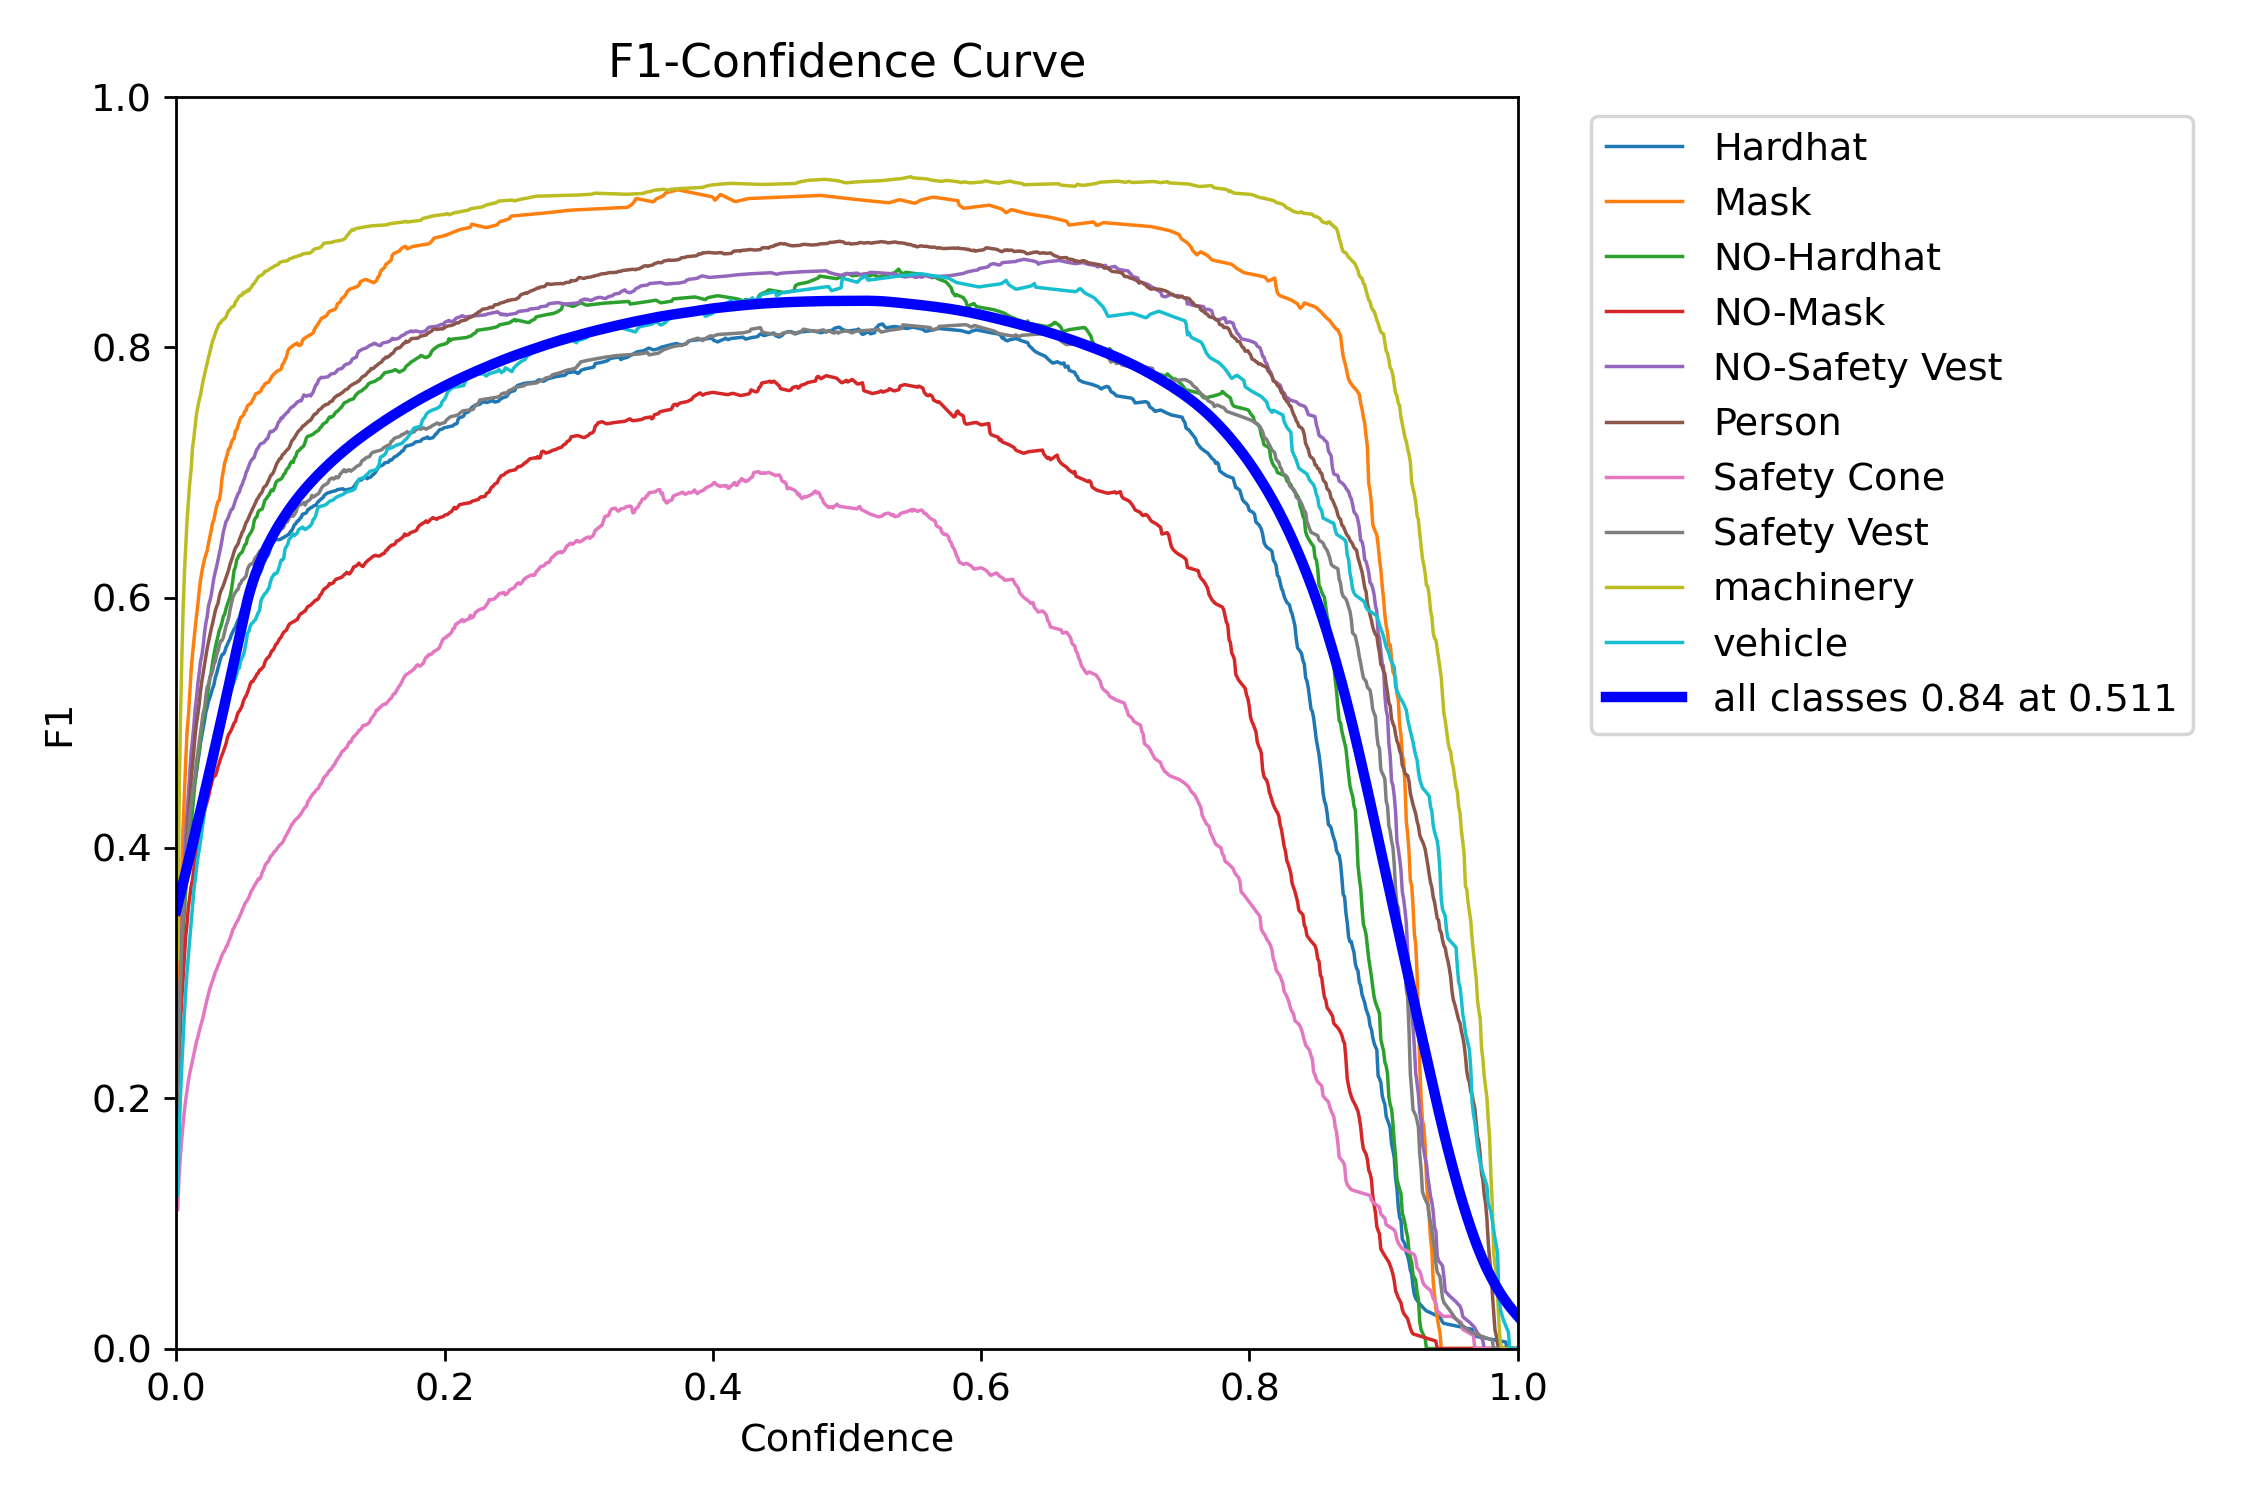
\includegraphics[width=\linewidth]{eval_test_tta_BoxF1_curve.png}\caption{F1}\end{subfigure}\hfill
\begin{subfigure}{0.49\linewidth}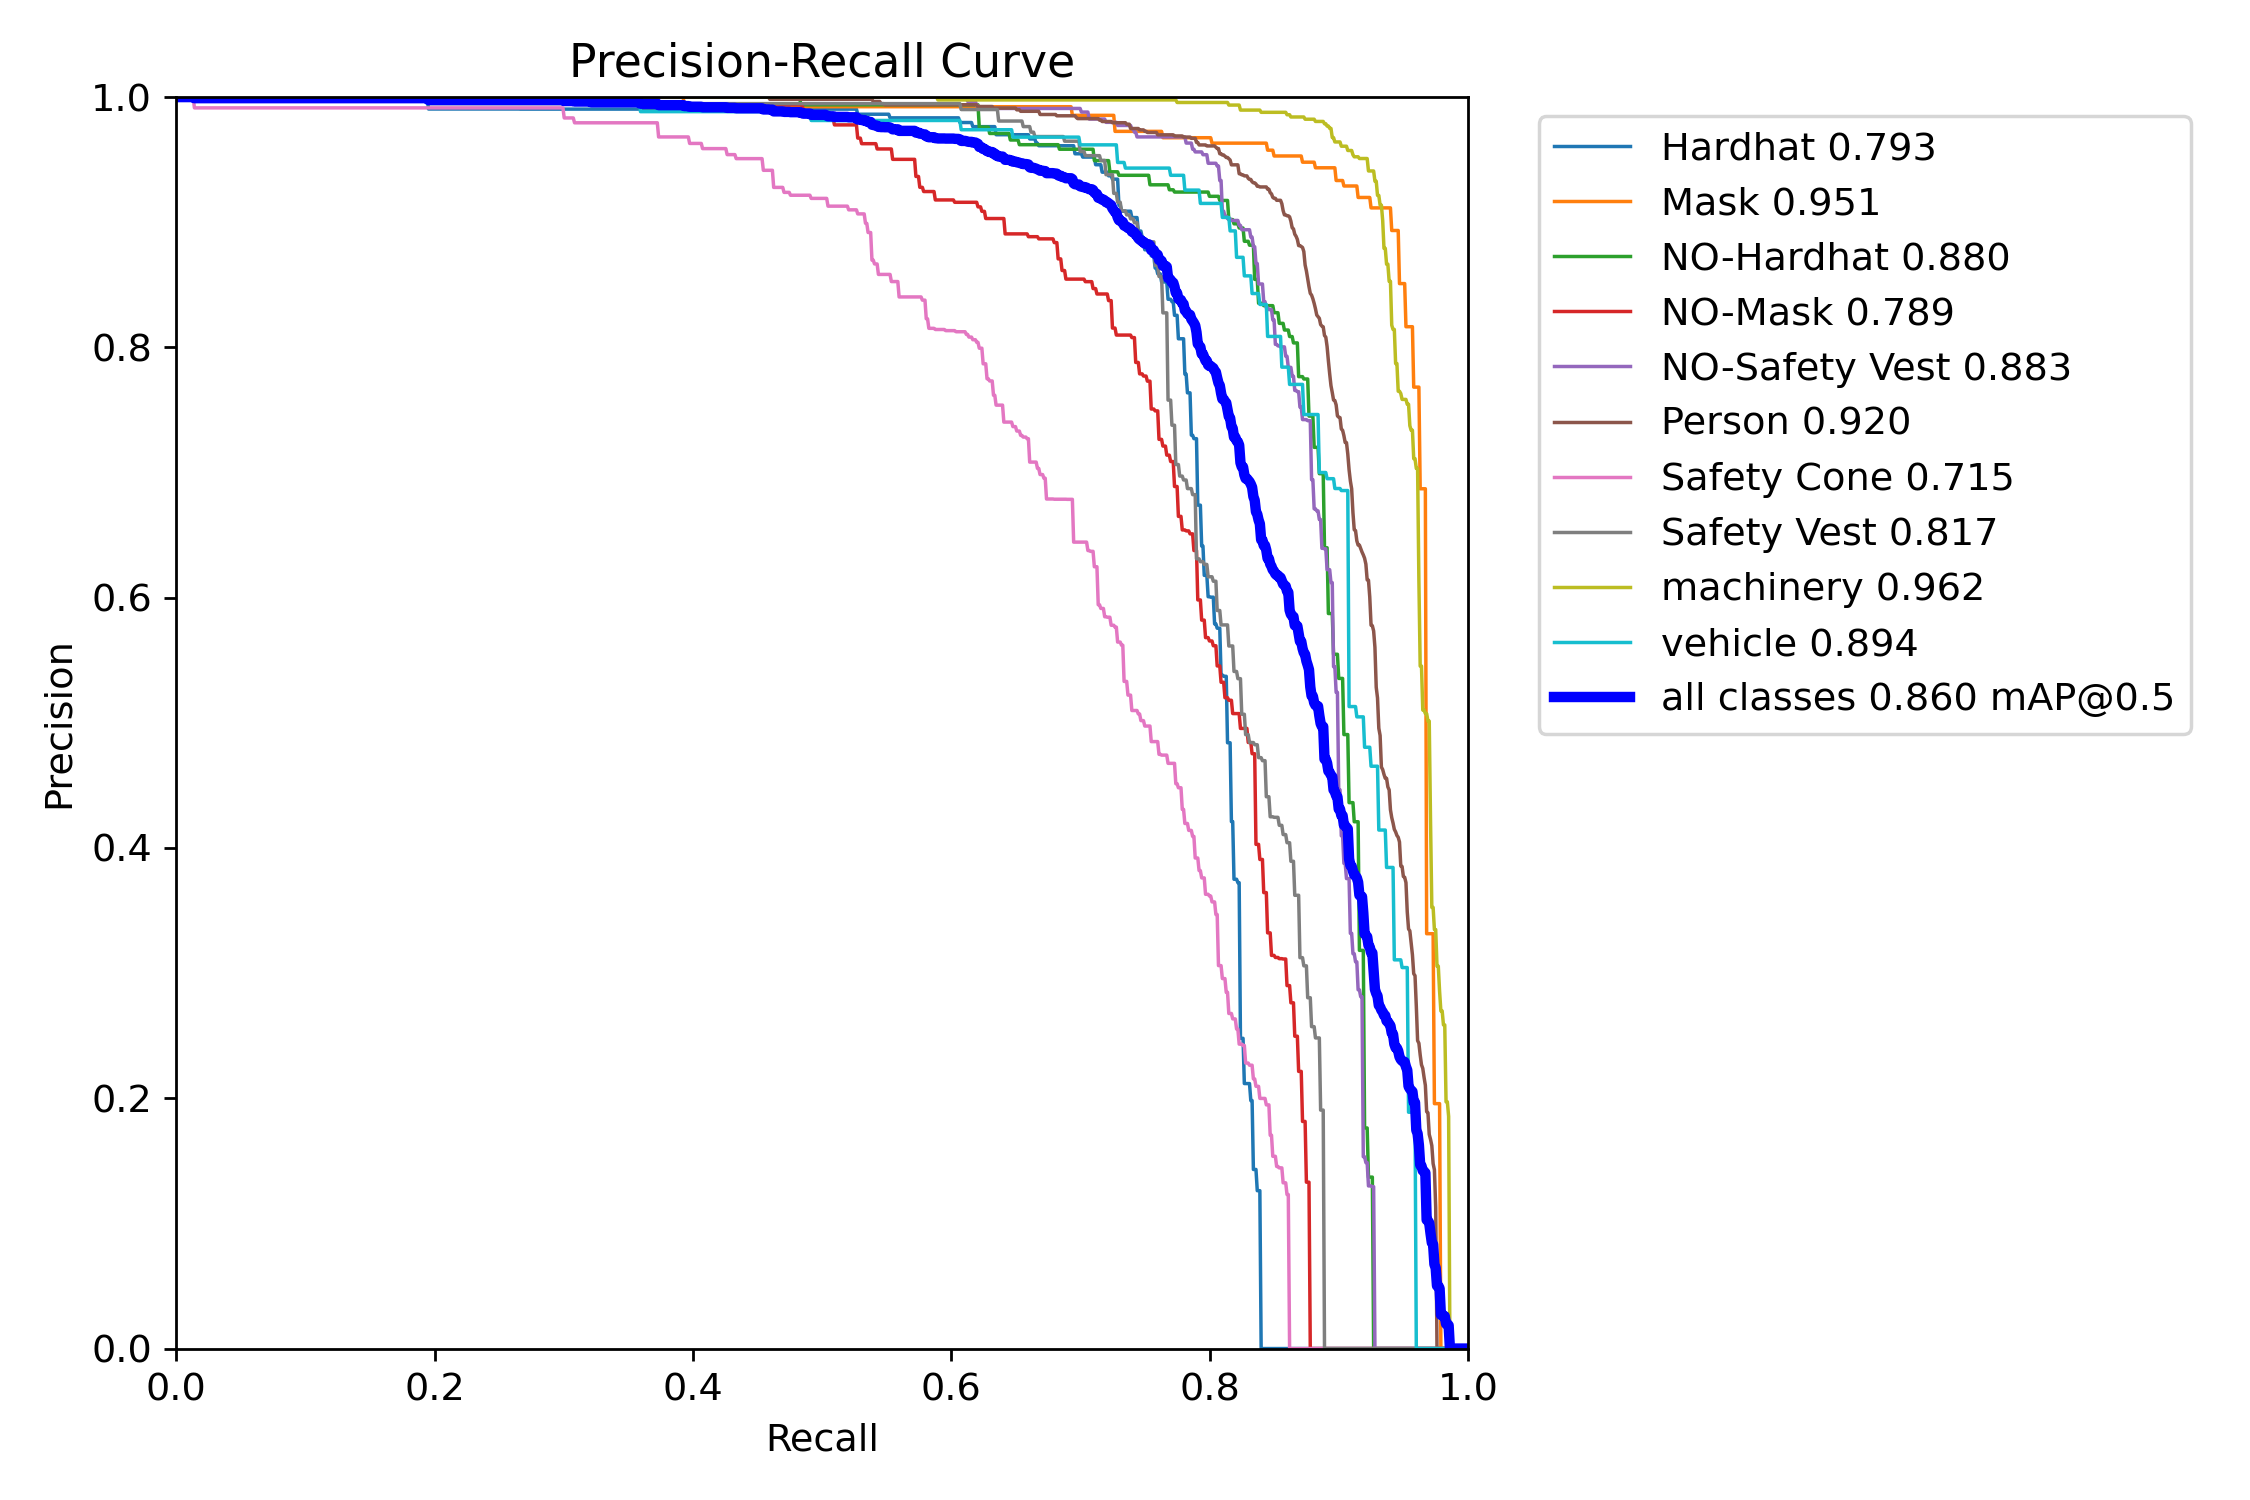
\includegraphics[width=\linewidth]{eval_test_tta_BoxPR_curve.png}\caption{Precision-recall}\end{subfigure}
\caption{Curves on the test split with flip and scale TTA.}
\label{fig:ttacurves}
\end{figure}

\begin{figure}[htbp]
\centering
\begin{subfigure}{0.49\linewidth}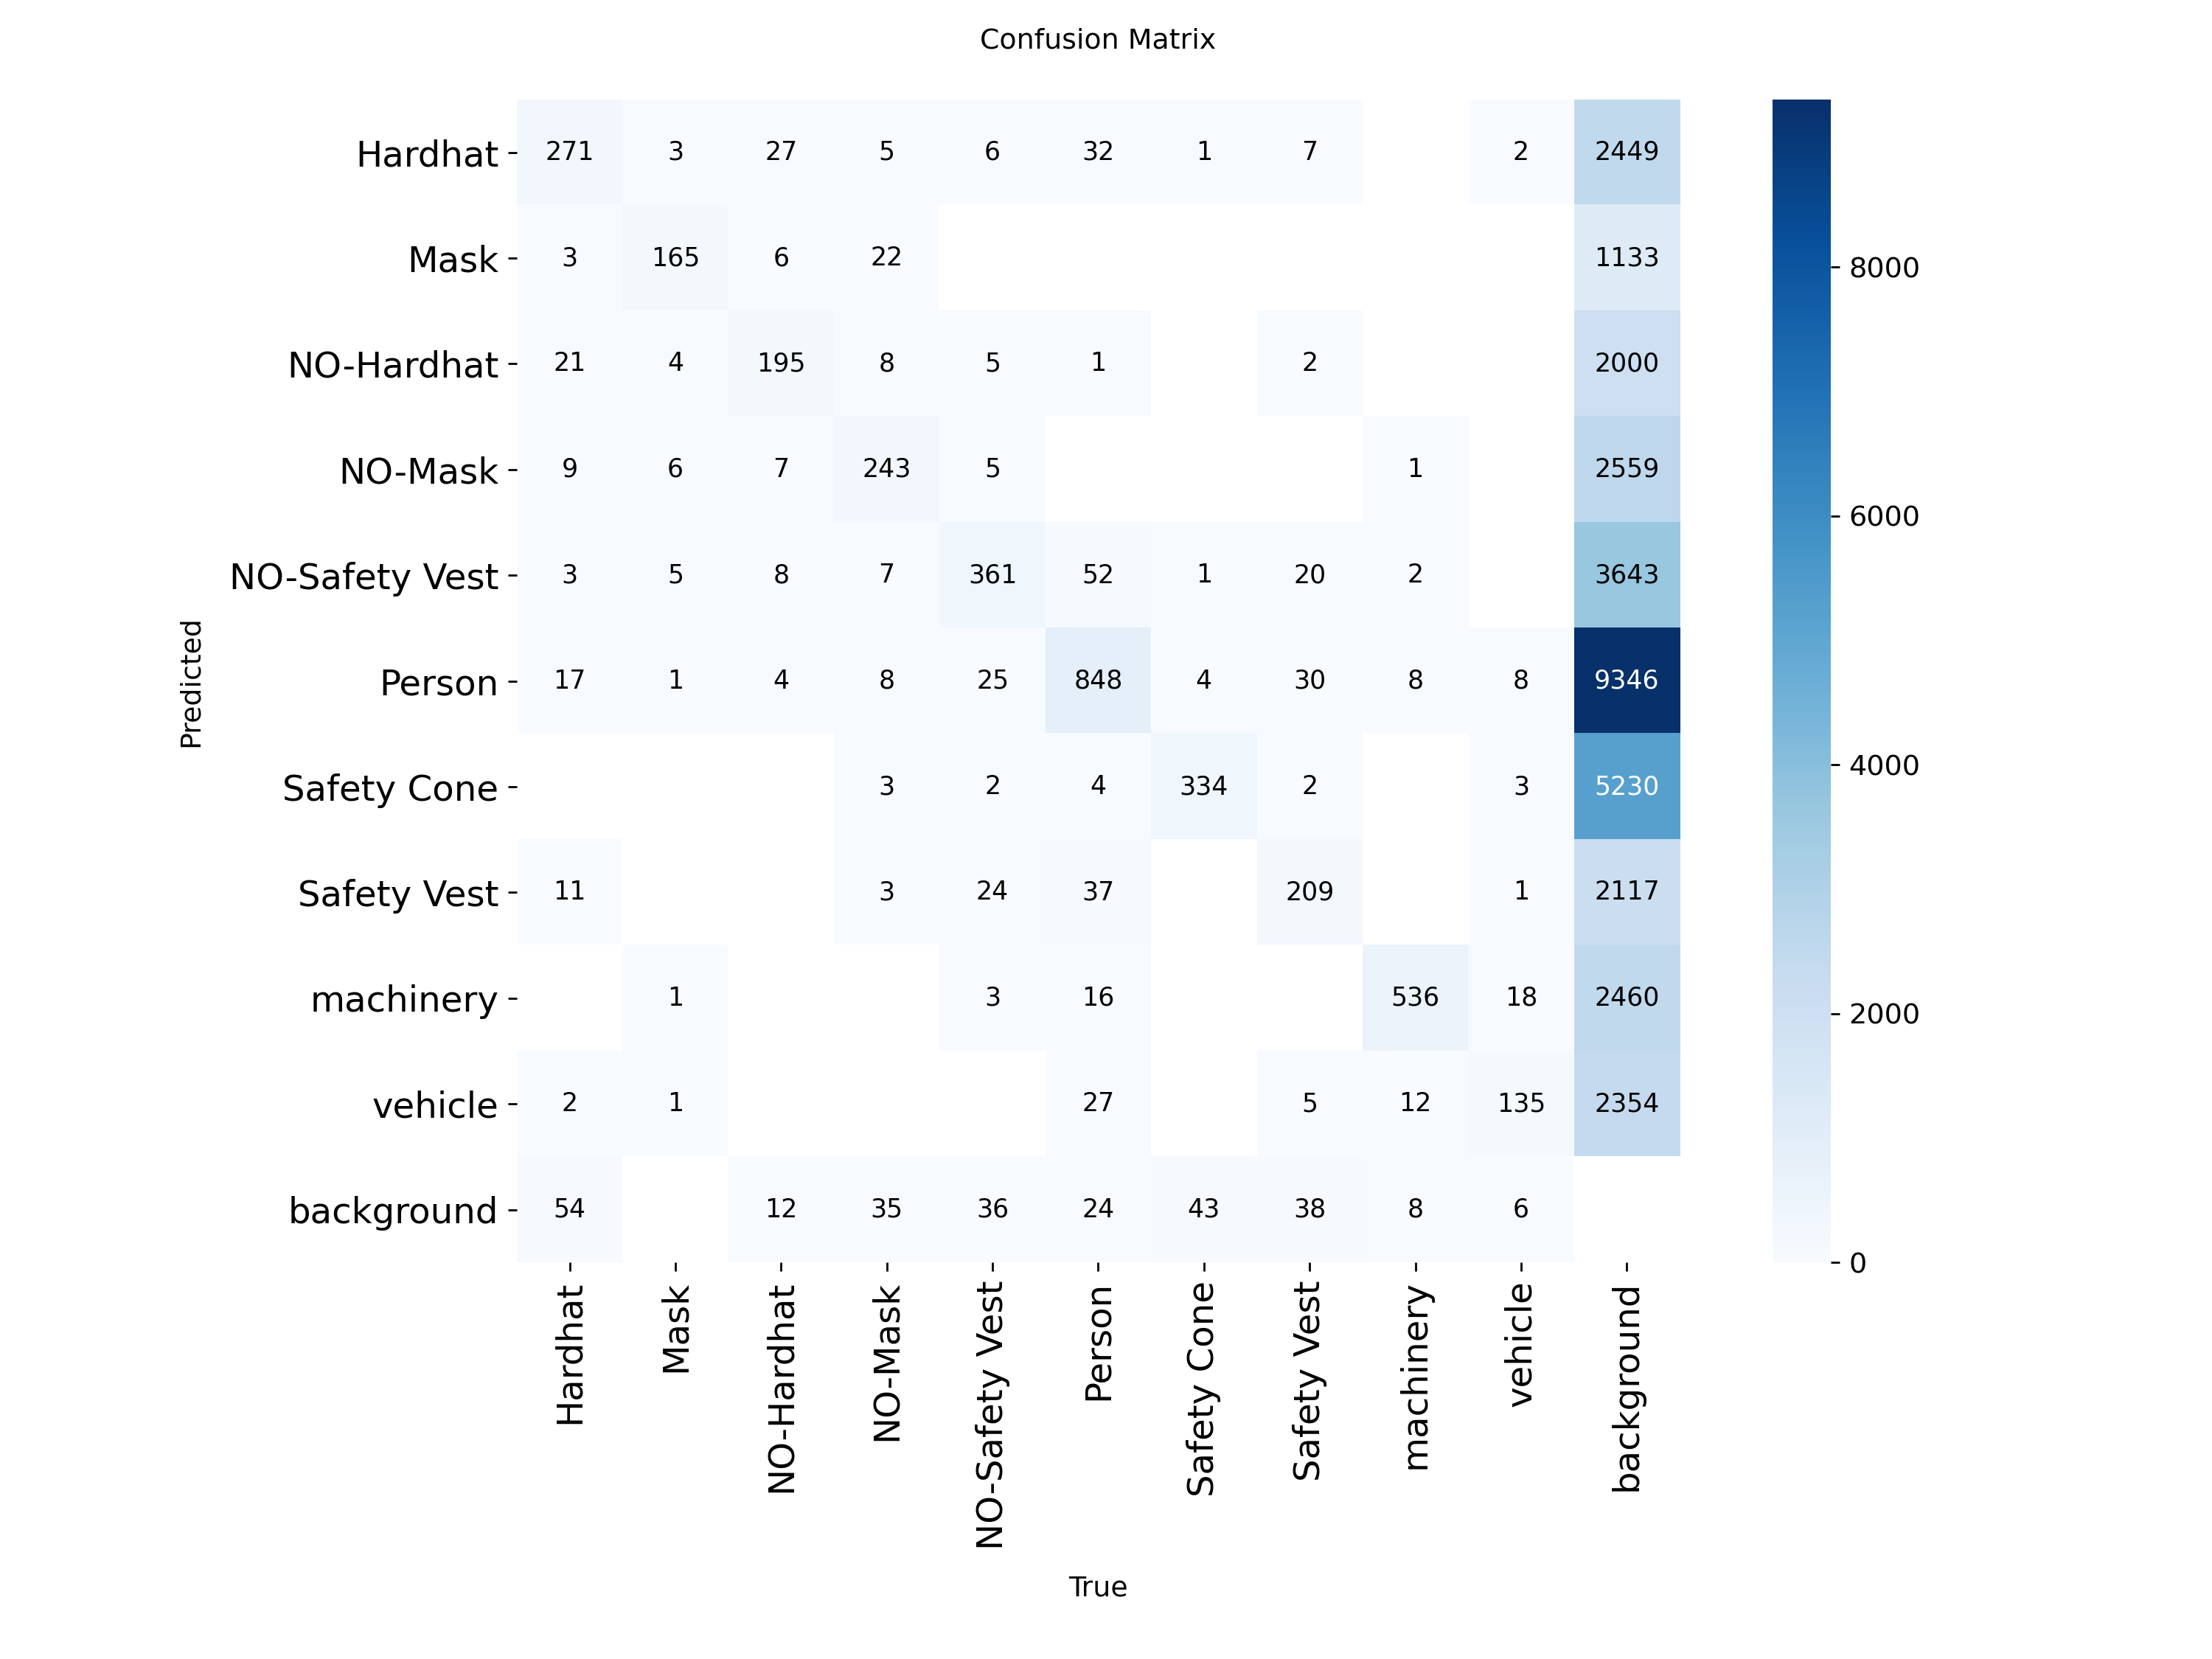
\includegraphics[width=\linewidth]{eval_test_tta_confusion_matrix.png}\caption{Counts}\end{subfigure}\hfill
\begin{subfigure}{0.49\linewidth}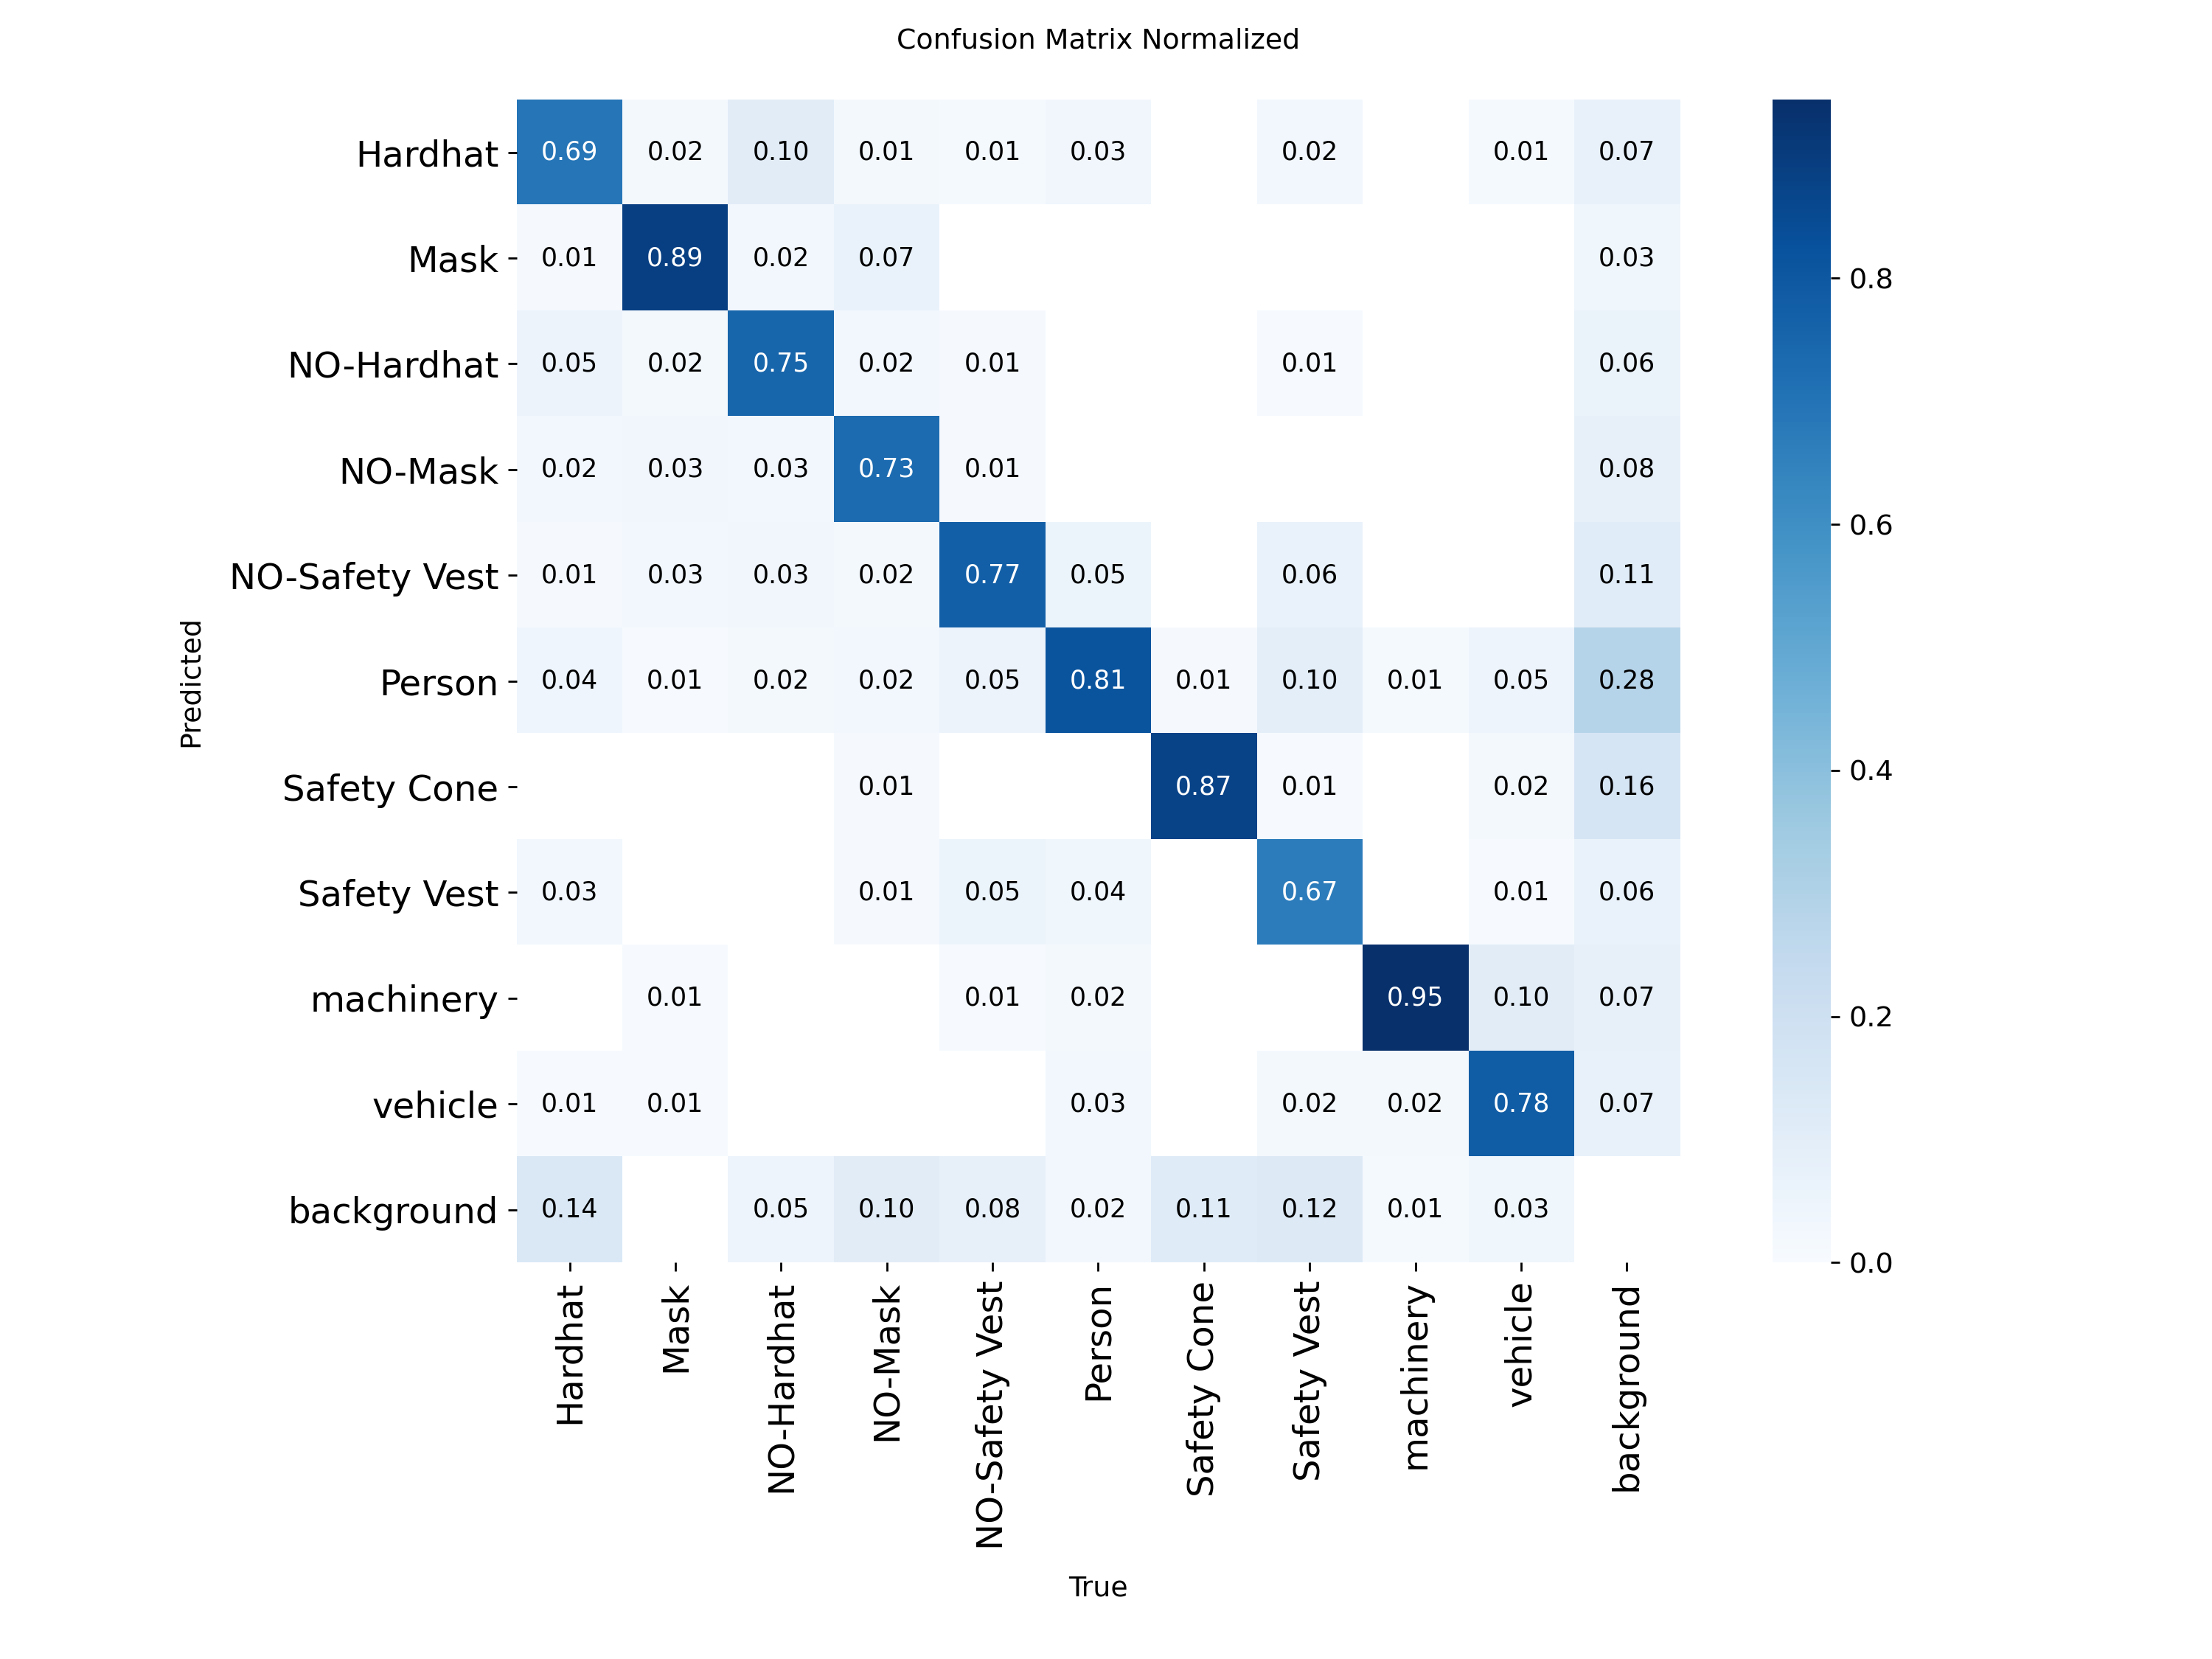
\includegraphics[width=\linewidth]{eval_test_tta_confusion_matrix_normalized.png}\caption{Normalised by true class}\end{subfigure}
\caption{Confusion matrices on the test split with flip and scale TTA.}
\label{fig:ttacm}
\end{figure}

\bibliographystyle{elsarticle-num}
\bibliography{refs}

\end{document}

\endinput
